\chapter*{Annexe} \markboth{Annexe}{Annexe}
\addcontentsline{toc}{chapter}{Annexe}


 \begin{figure*}[htp]
   \centering
   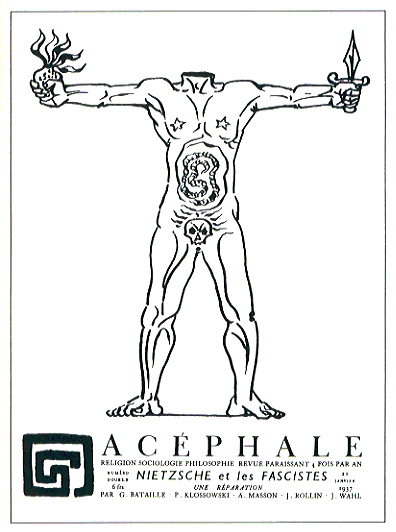
\includegraphics[width=\textwidth,height=\textheight,keepaspectratio]{Annexe/acephalemasson.jpg}
	\caption{\cite{memoiremonde}}\label{fig:Acephale}
\end{figure*}


  \begin{figure*}[htp]
   \centering
   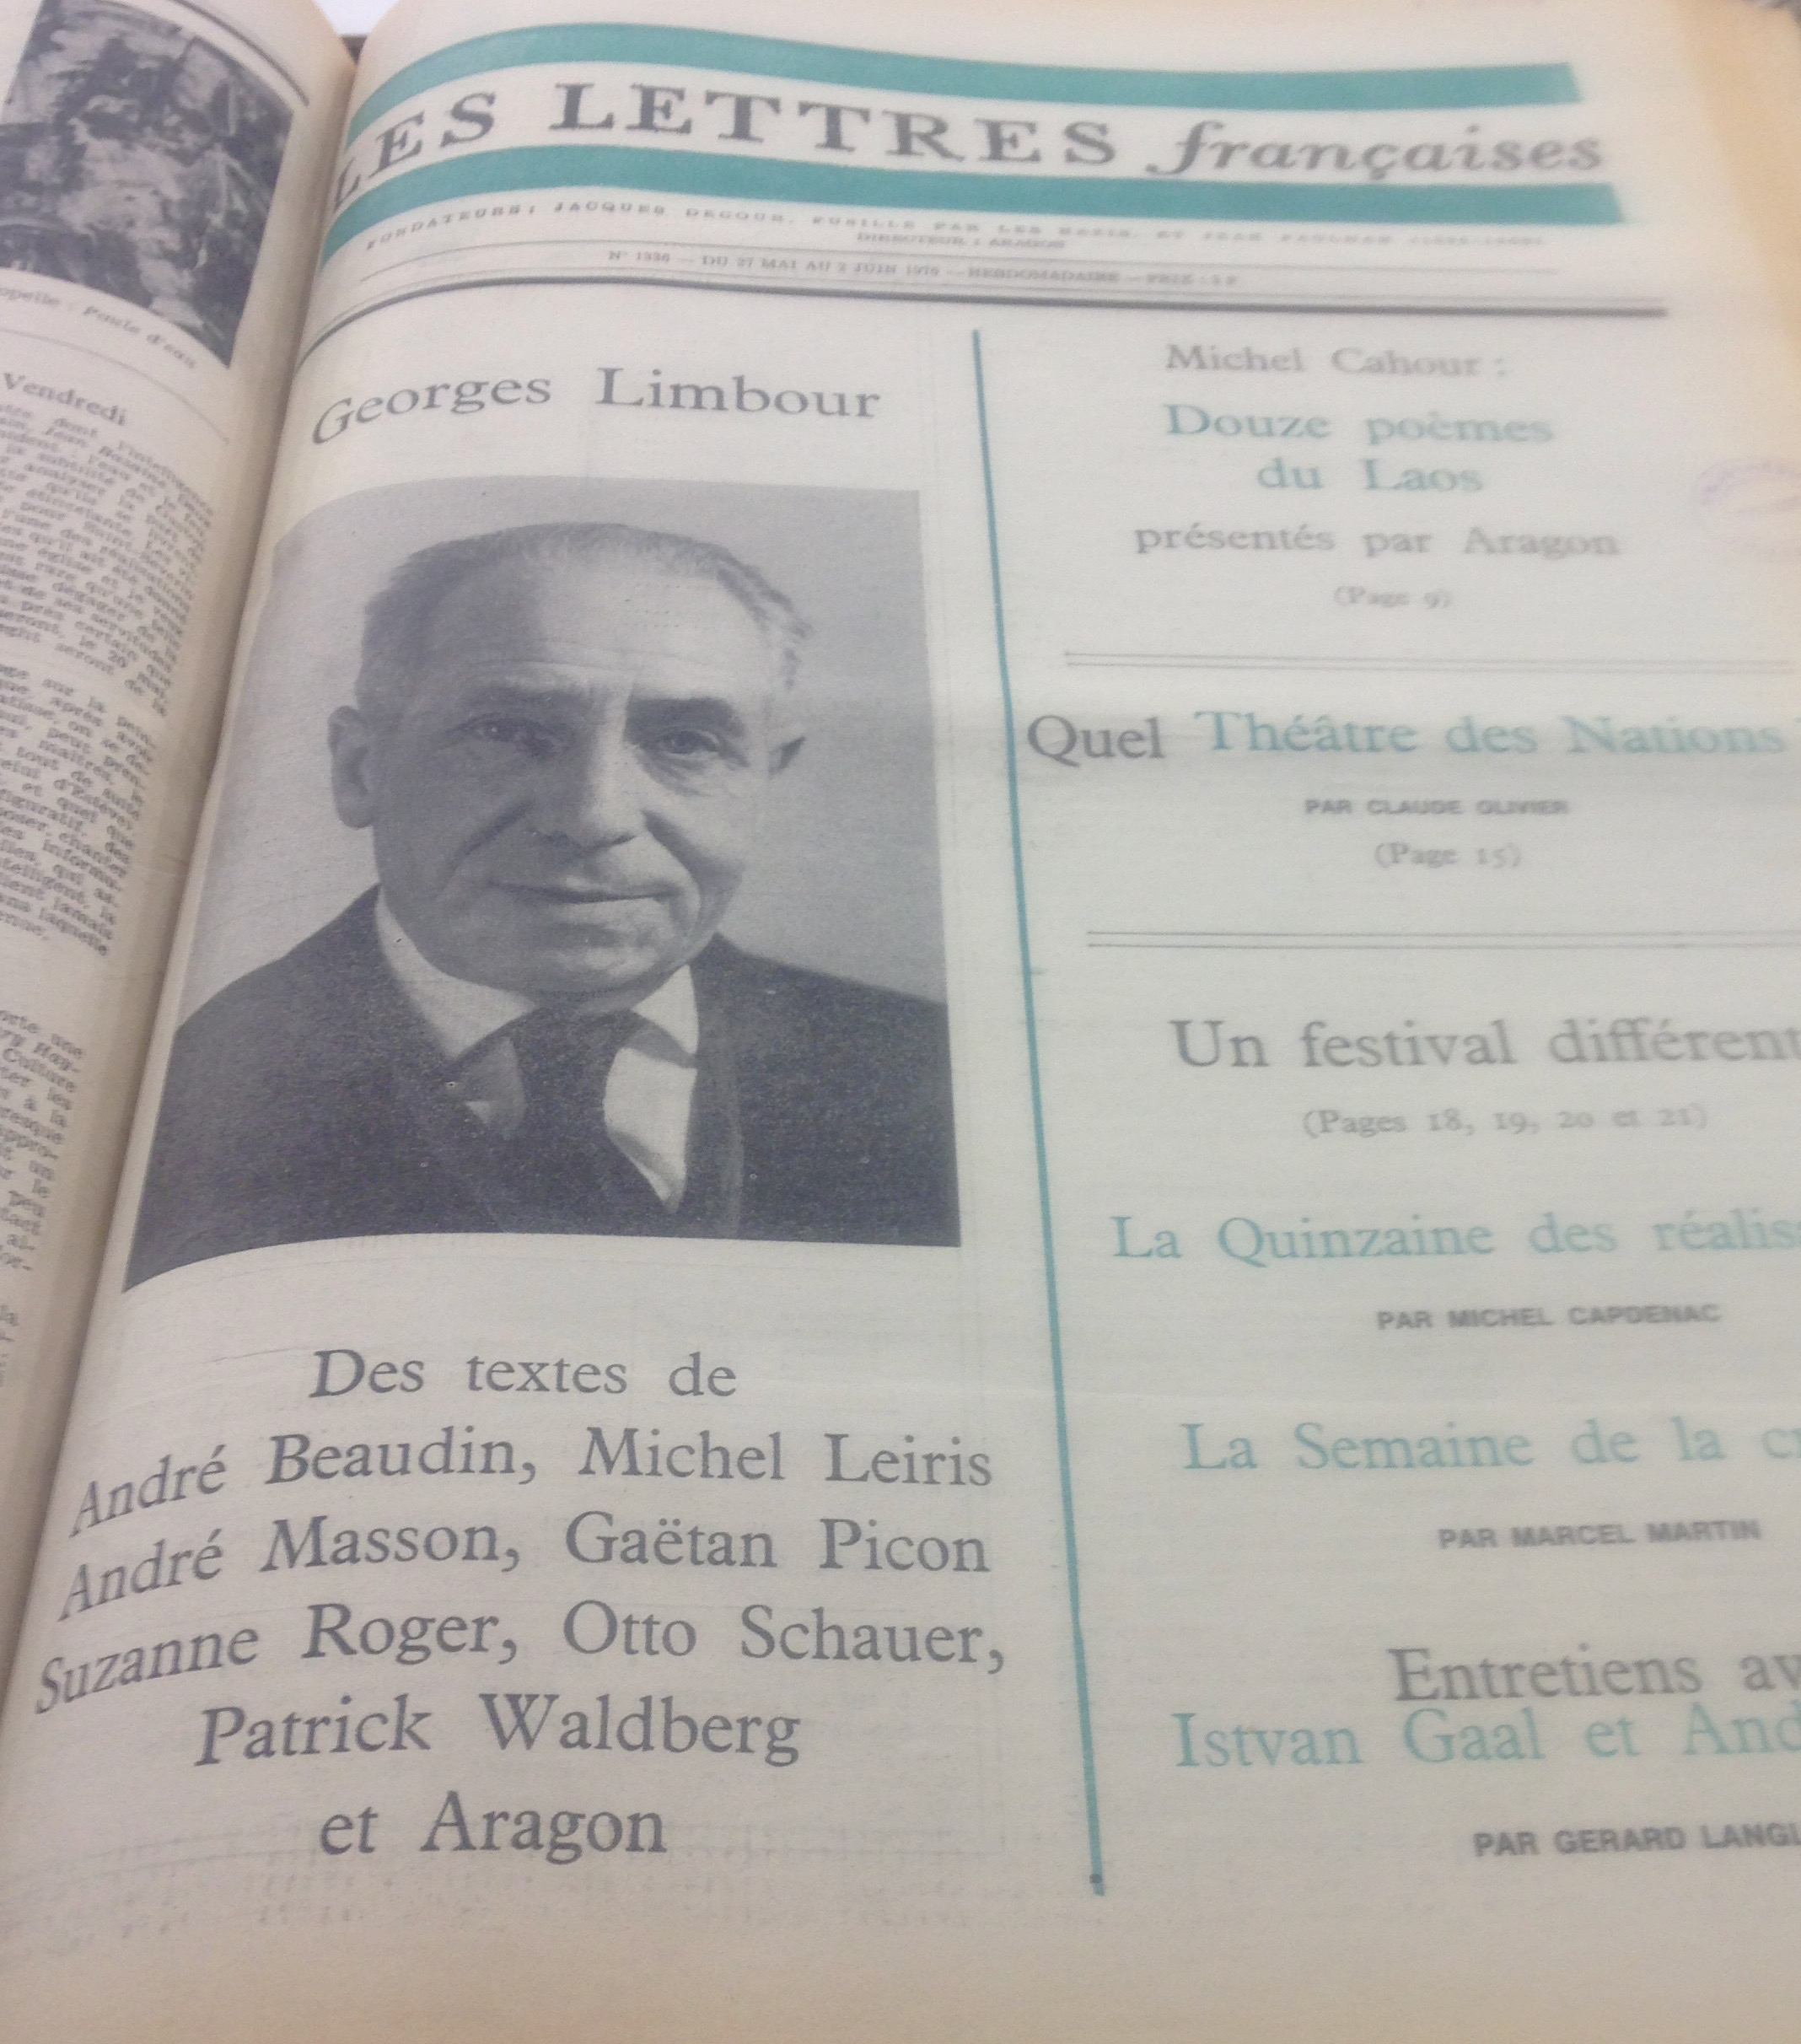
\includegraphics[width=\textwidth,height=\textheight,keepaspectratio]{Annexe/Image20.jpg}
	\caption{\cite{journallimbour}}\label{fig:limbour2}
    \end{figure*}

  \begin{figure*}[htp]
   \centering
   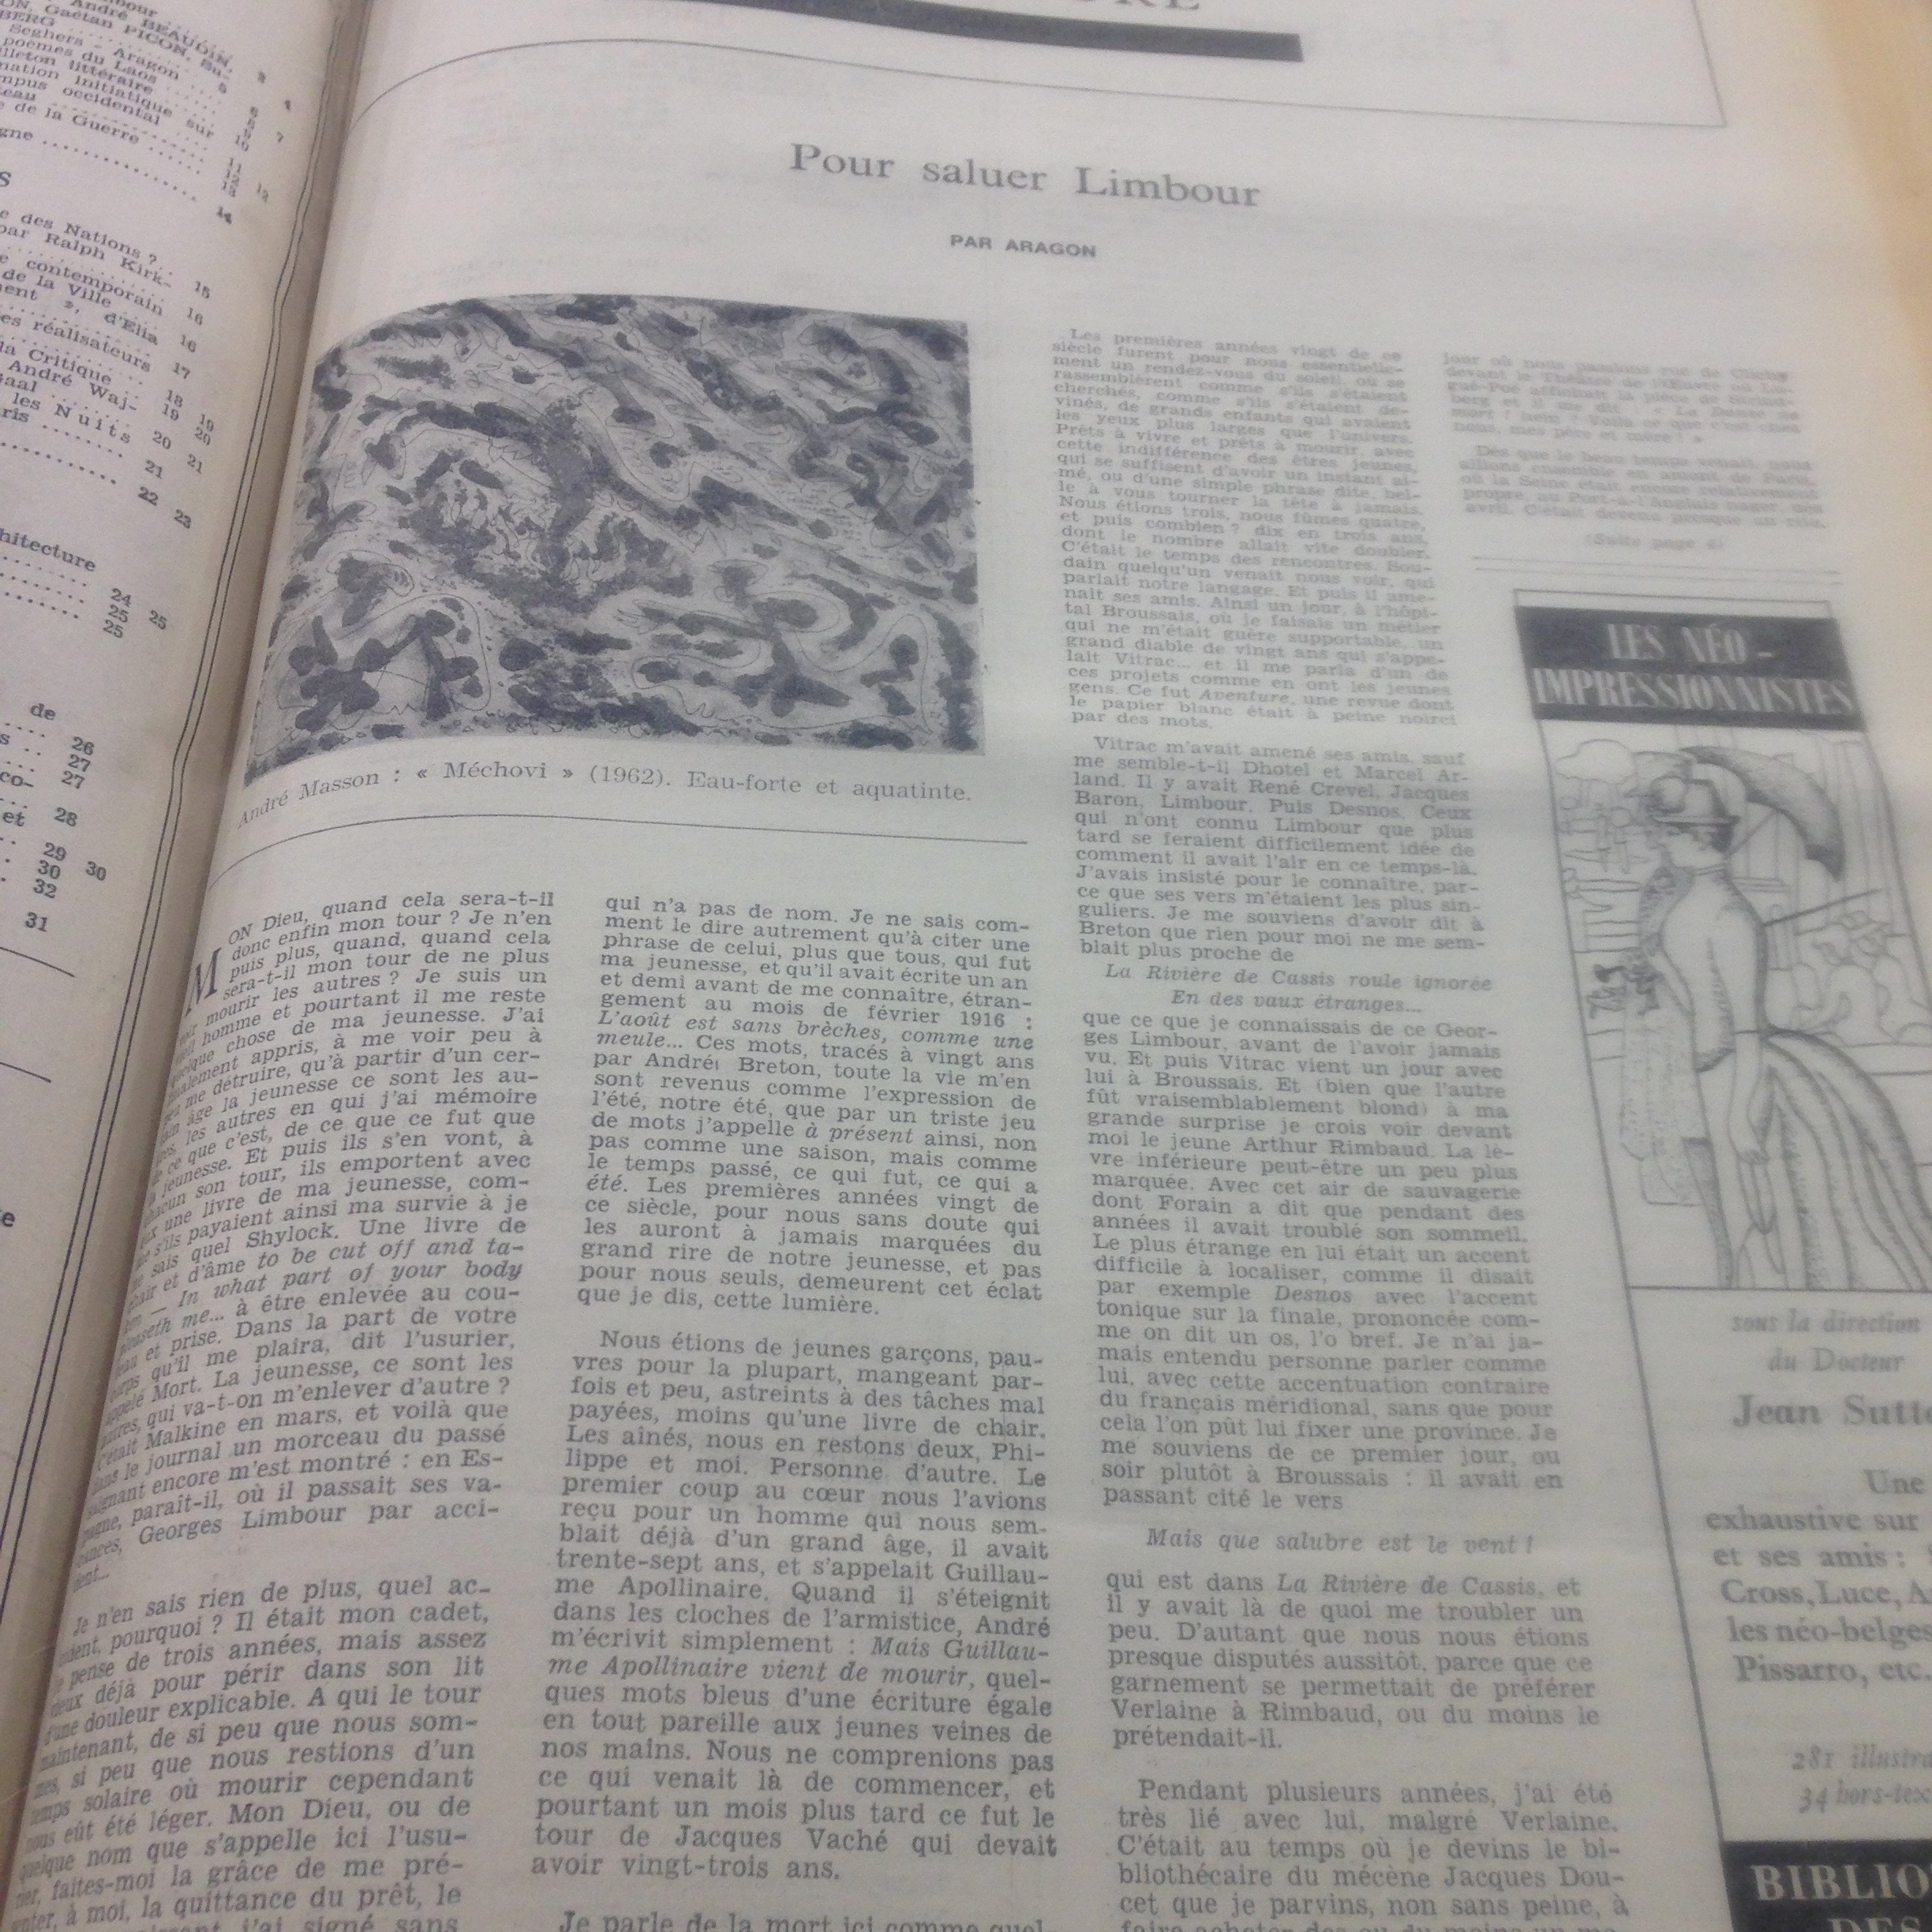
\includegraphics[width=\textwidth,height=\textheight,keepaspectratio]{Annexe/Image6.jpg}
	\caption{\cite{journallimbour}}\label{fig:journallimbour}
    \end{figure*}

    \begin{figure*}[htp]
   \centering
   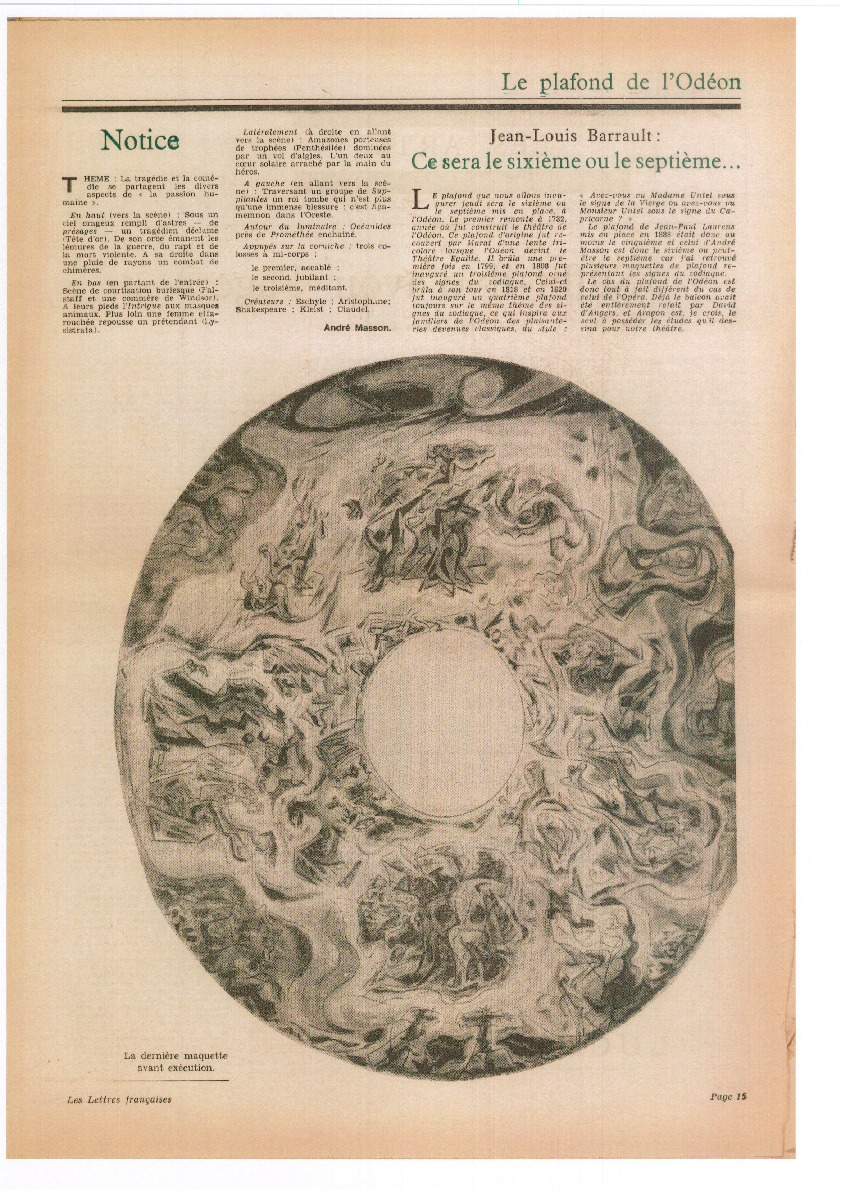
\includegraphics[width=\textwidth,height=\textheight,keepaspectratio]{Annexe/Image11.jpg}
	\caption{\cite{plafondodeon}}\label{fig:odeon}
    \end{figure*}


  \begin{figure*}[htp]
   \centering
   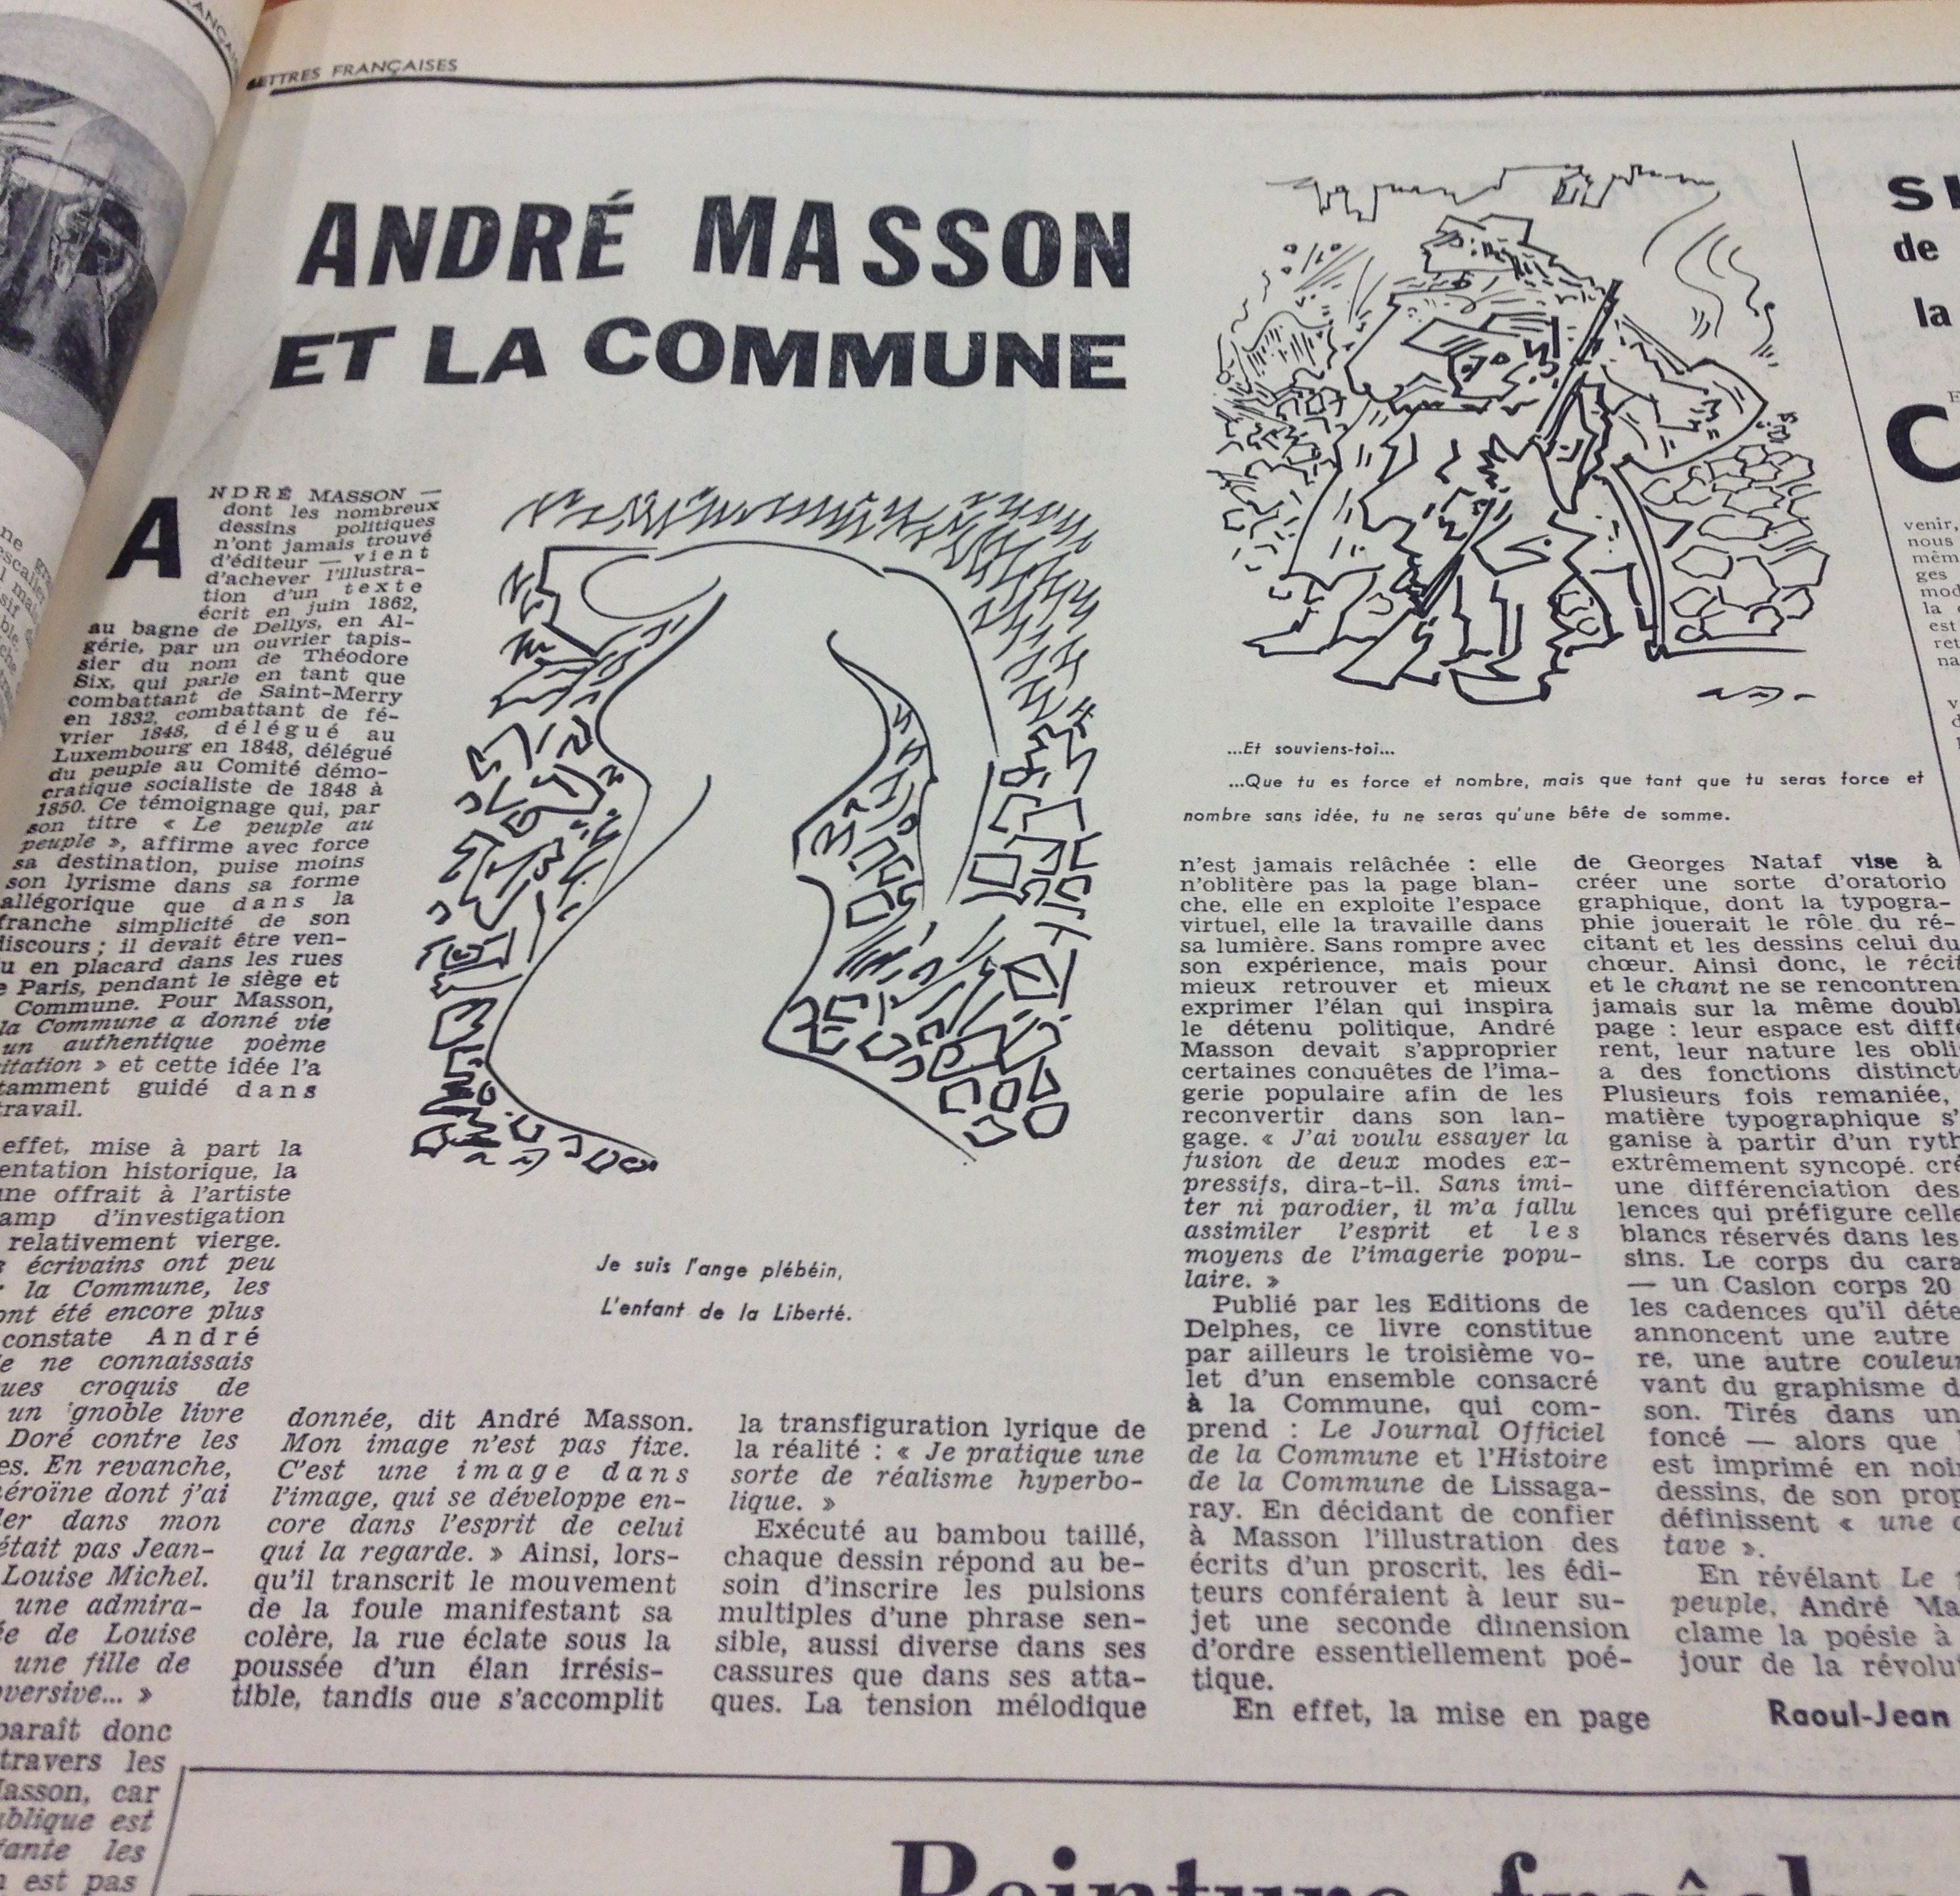
\includegraphics[width=\textwidth,height=\textheight,keepaspectratio]{pagecommune.jpg}
	\caption{\cite{commune}}\label{fig:Massoncommune}
    \end{figure*}



   \begin{figure*}[htp]
   \centering
   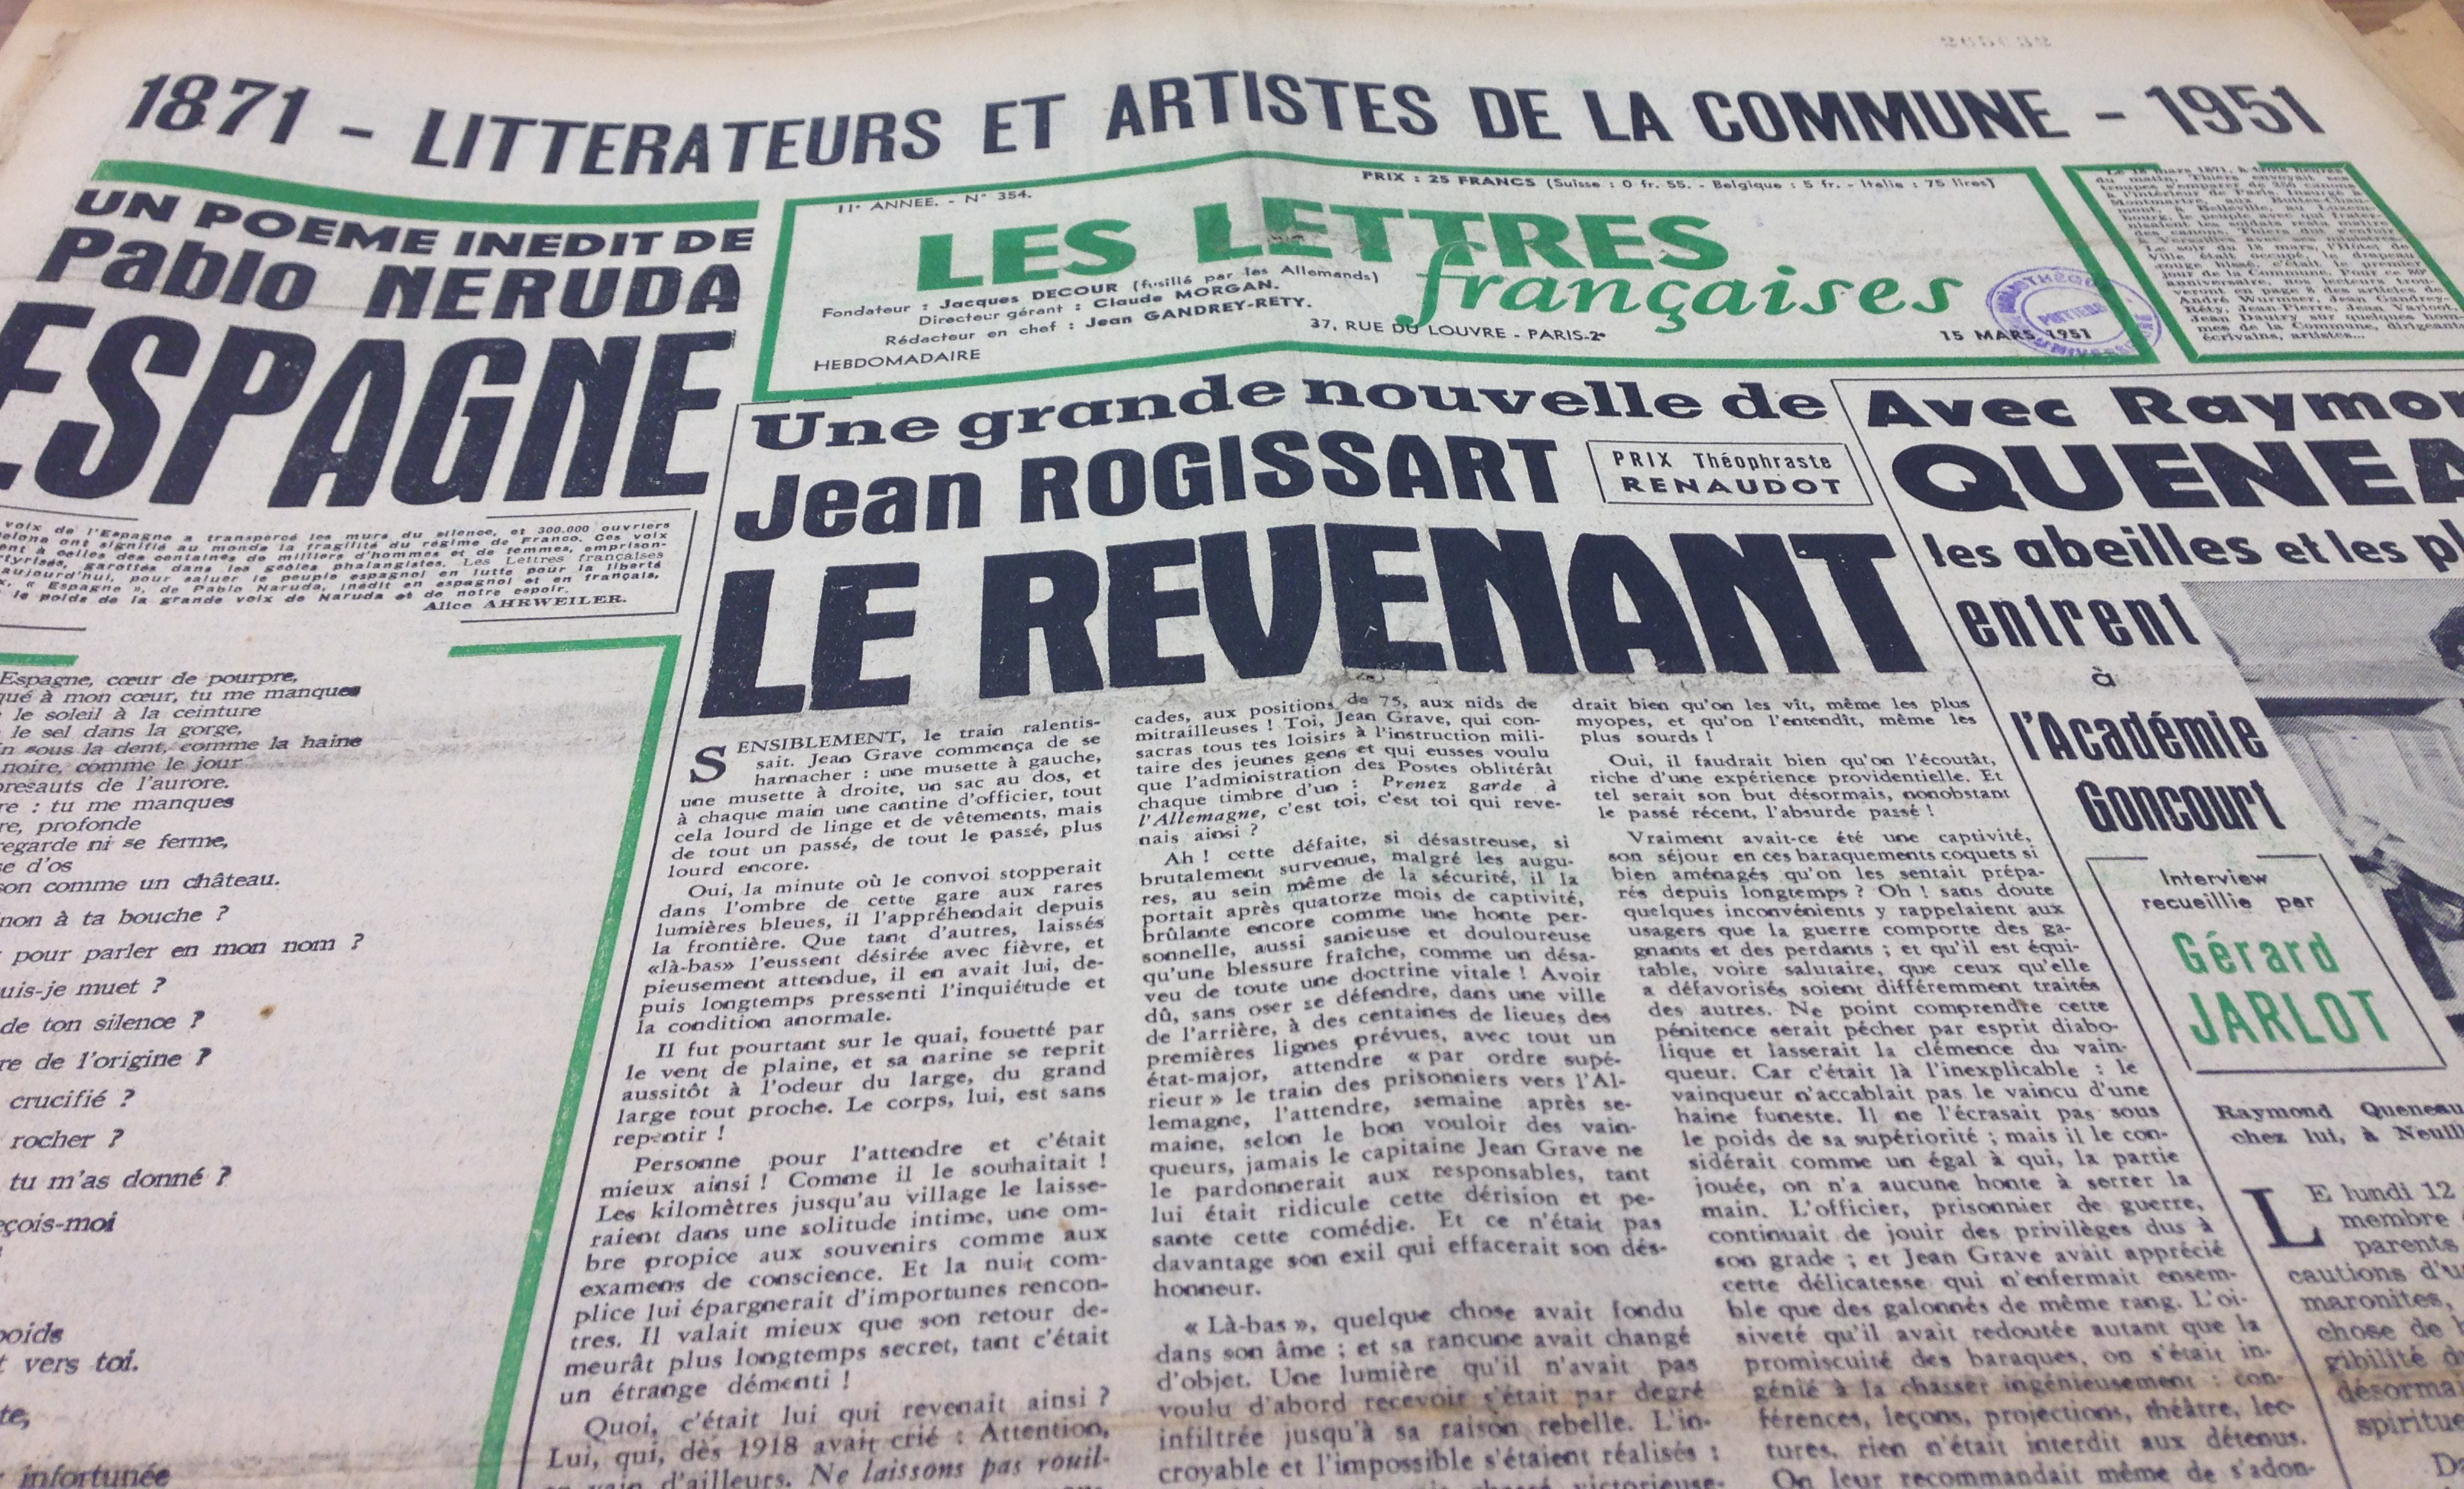
\includegraphics[width=\textwidth,height=\textheight,keepaspectratio]{Annexe/Image2.jpg}
	\caption{\cite{courbetcommunard}}\label{fig:commune}
    \end{figure*}


  \begin{figure*}[htp]
   \centering
   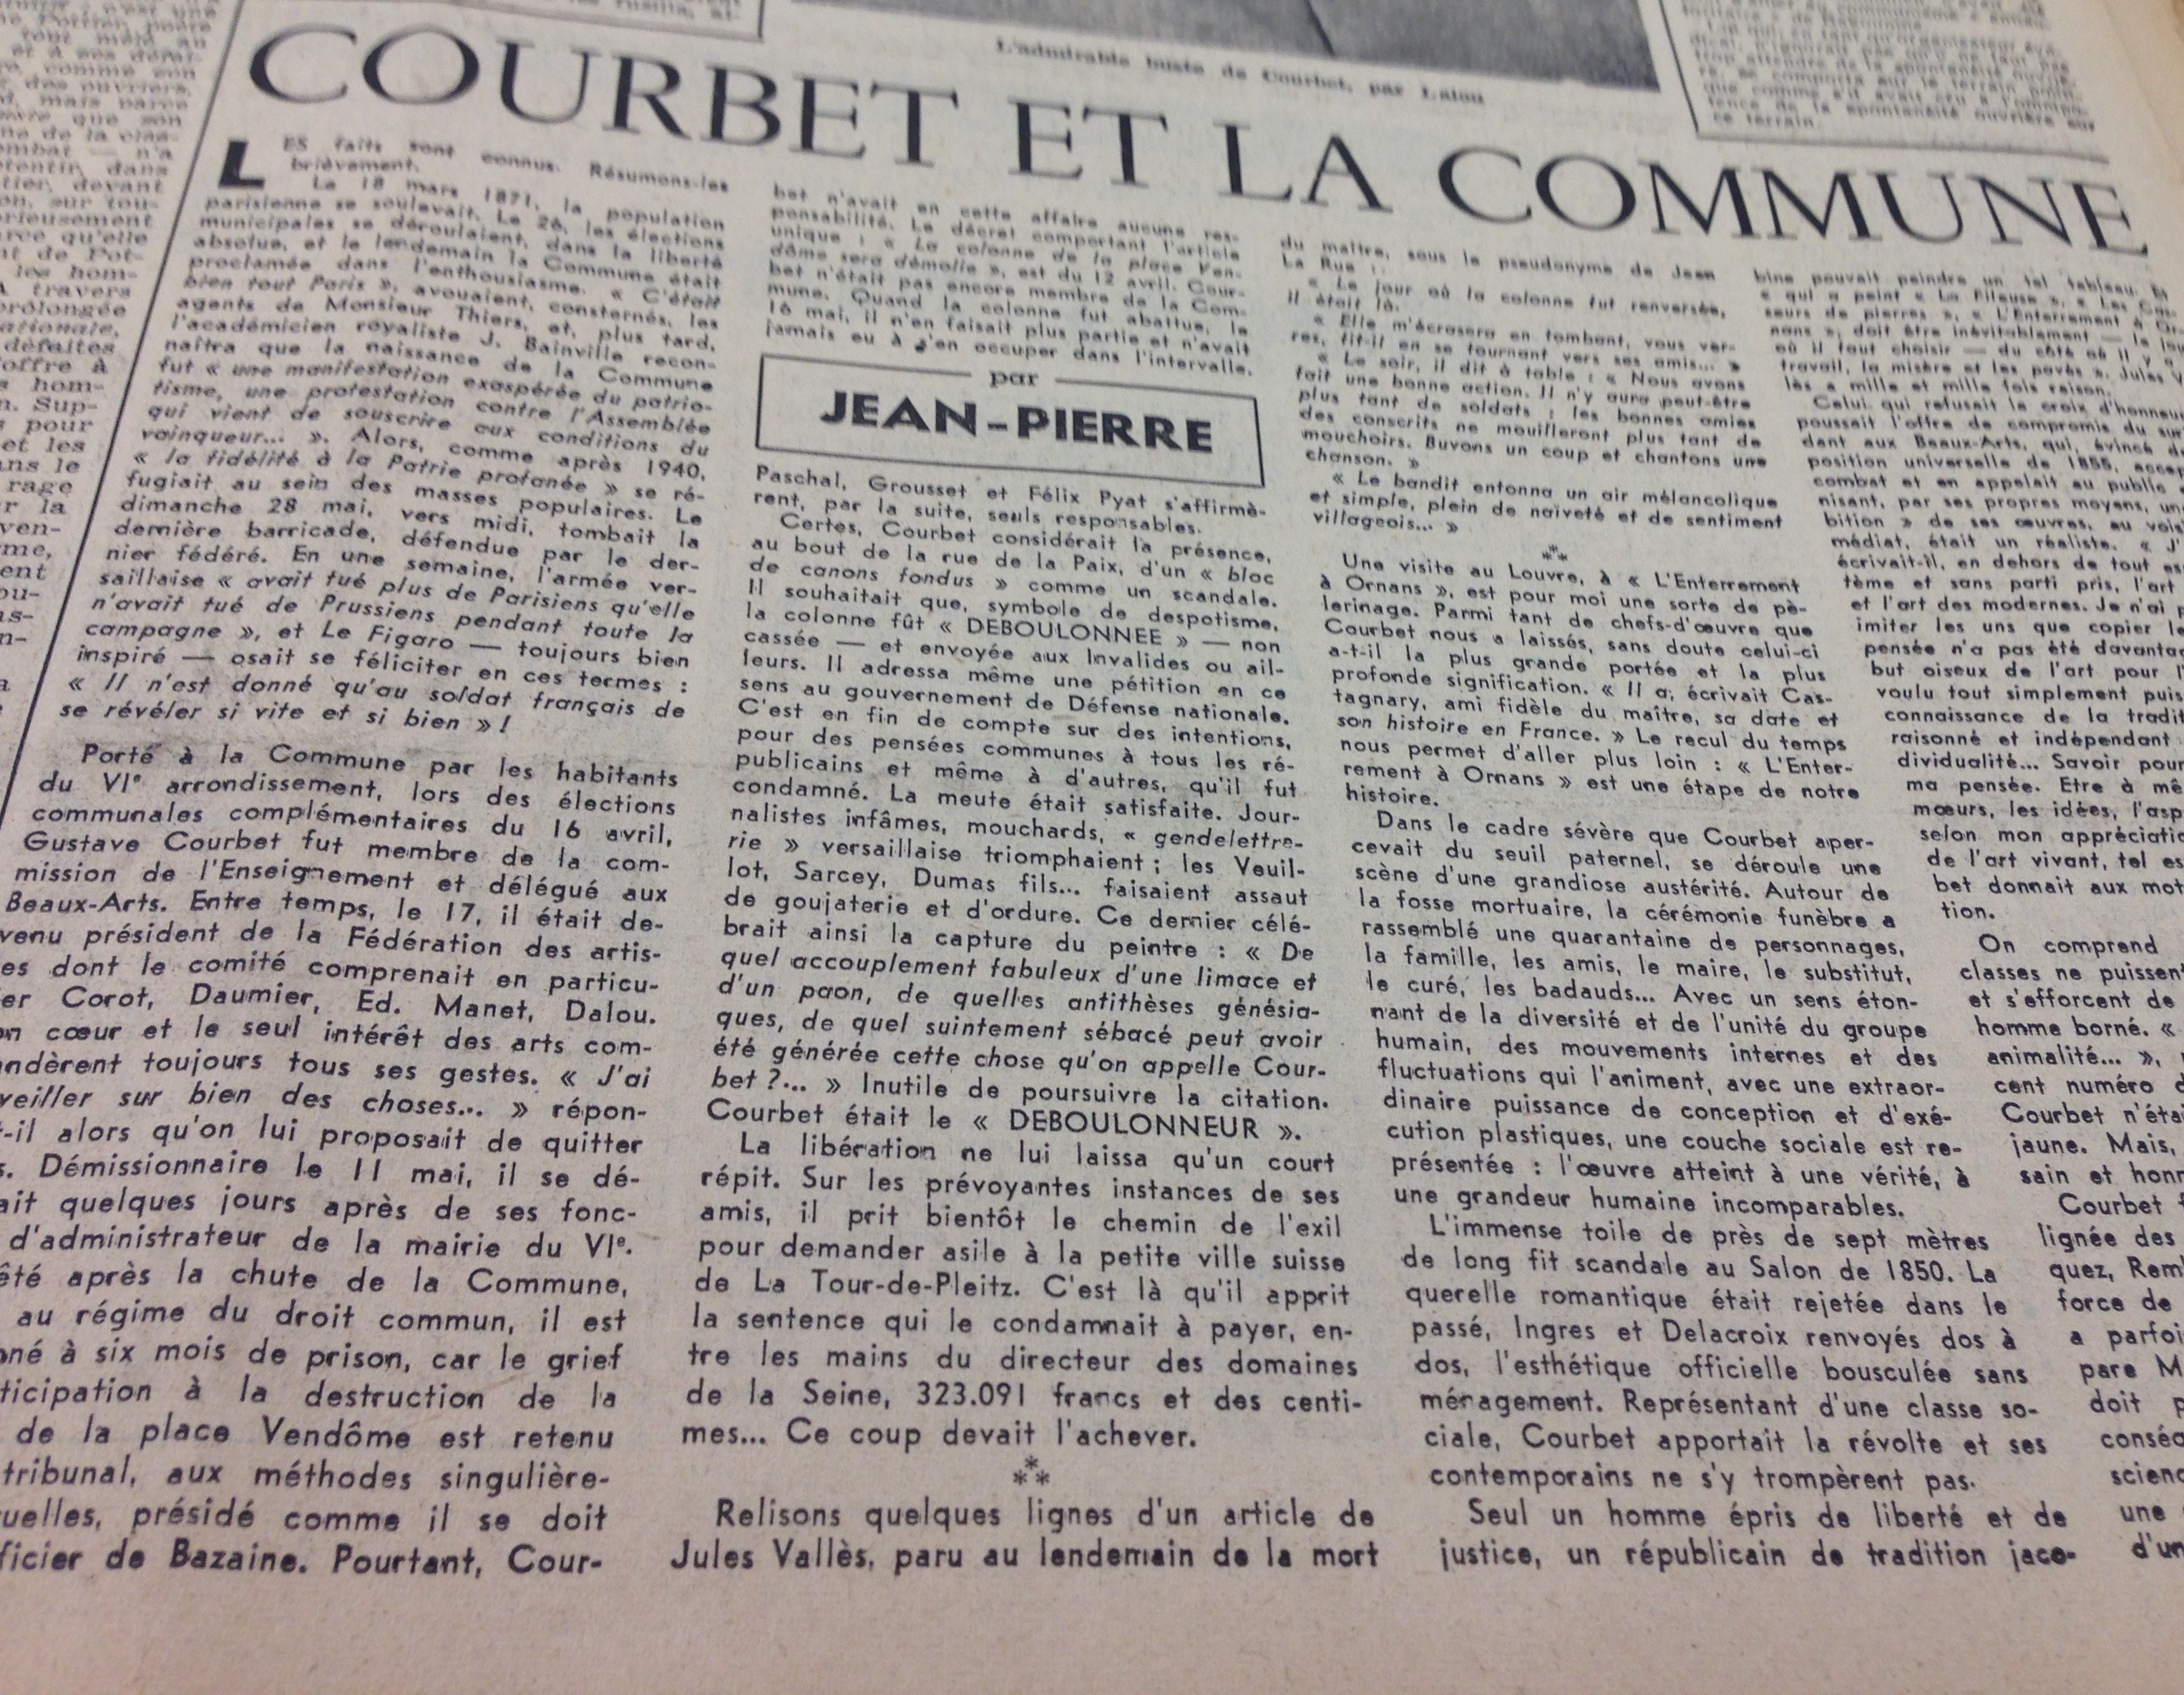
\includegraphics[width=\textwidth,height=\textheight,keepaspectratio]{Annexe/Image15.jpg}
	\caption{\cite{courbetcommunard}}\label{fig:courbetcommune}
    \end{figure*}


   \begin{figure*}[htp]
   \centering
   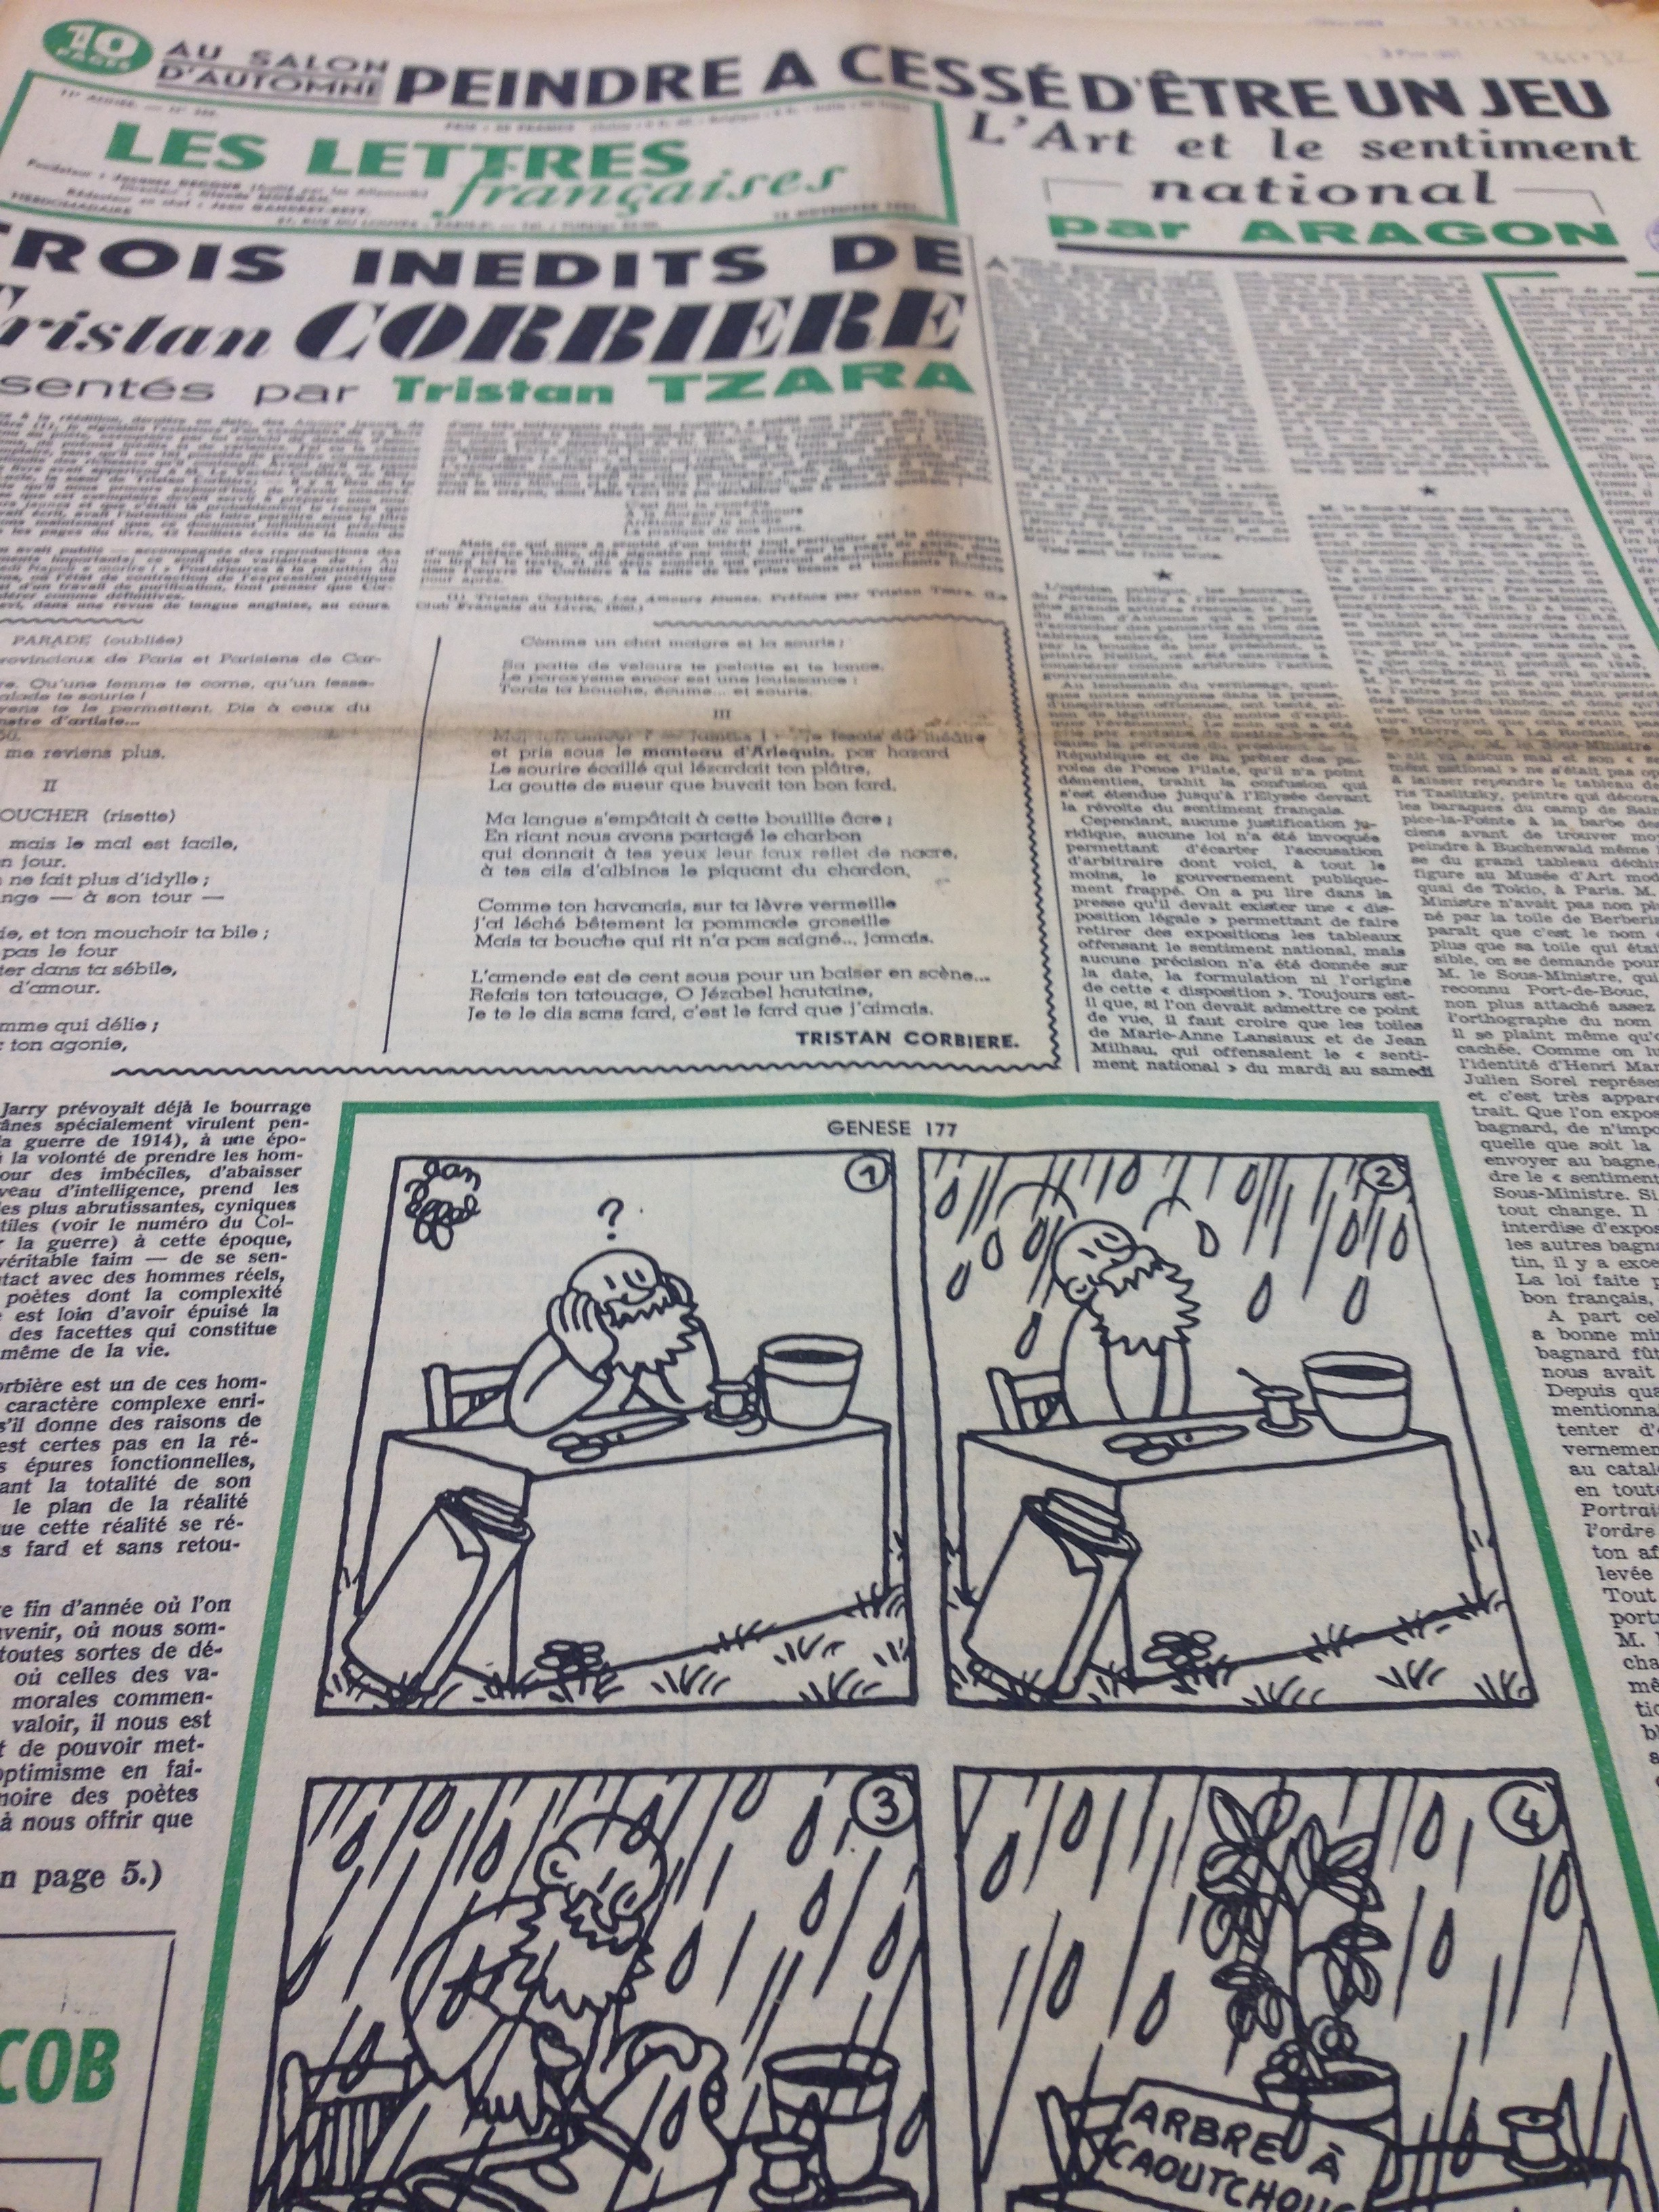
\includegraphics[width=\textwidth,height=\textheight,keepaspectratio]{Annexe/Image25.jpg}
	\caption{\cite{peindrefinjeu}}\label{fig:peindrefinjeu}
    \end{figure*}


   \begin{figure*}[htp]
   \centering
   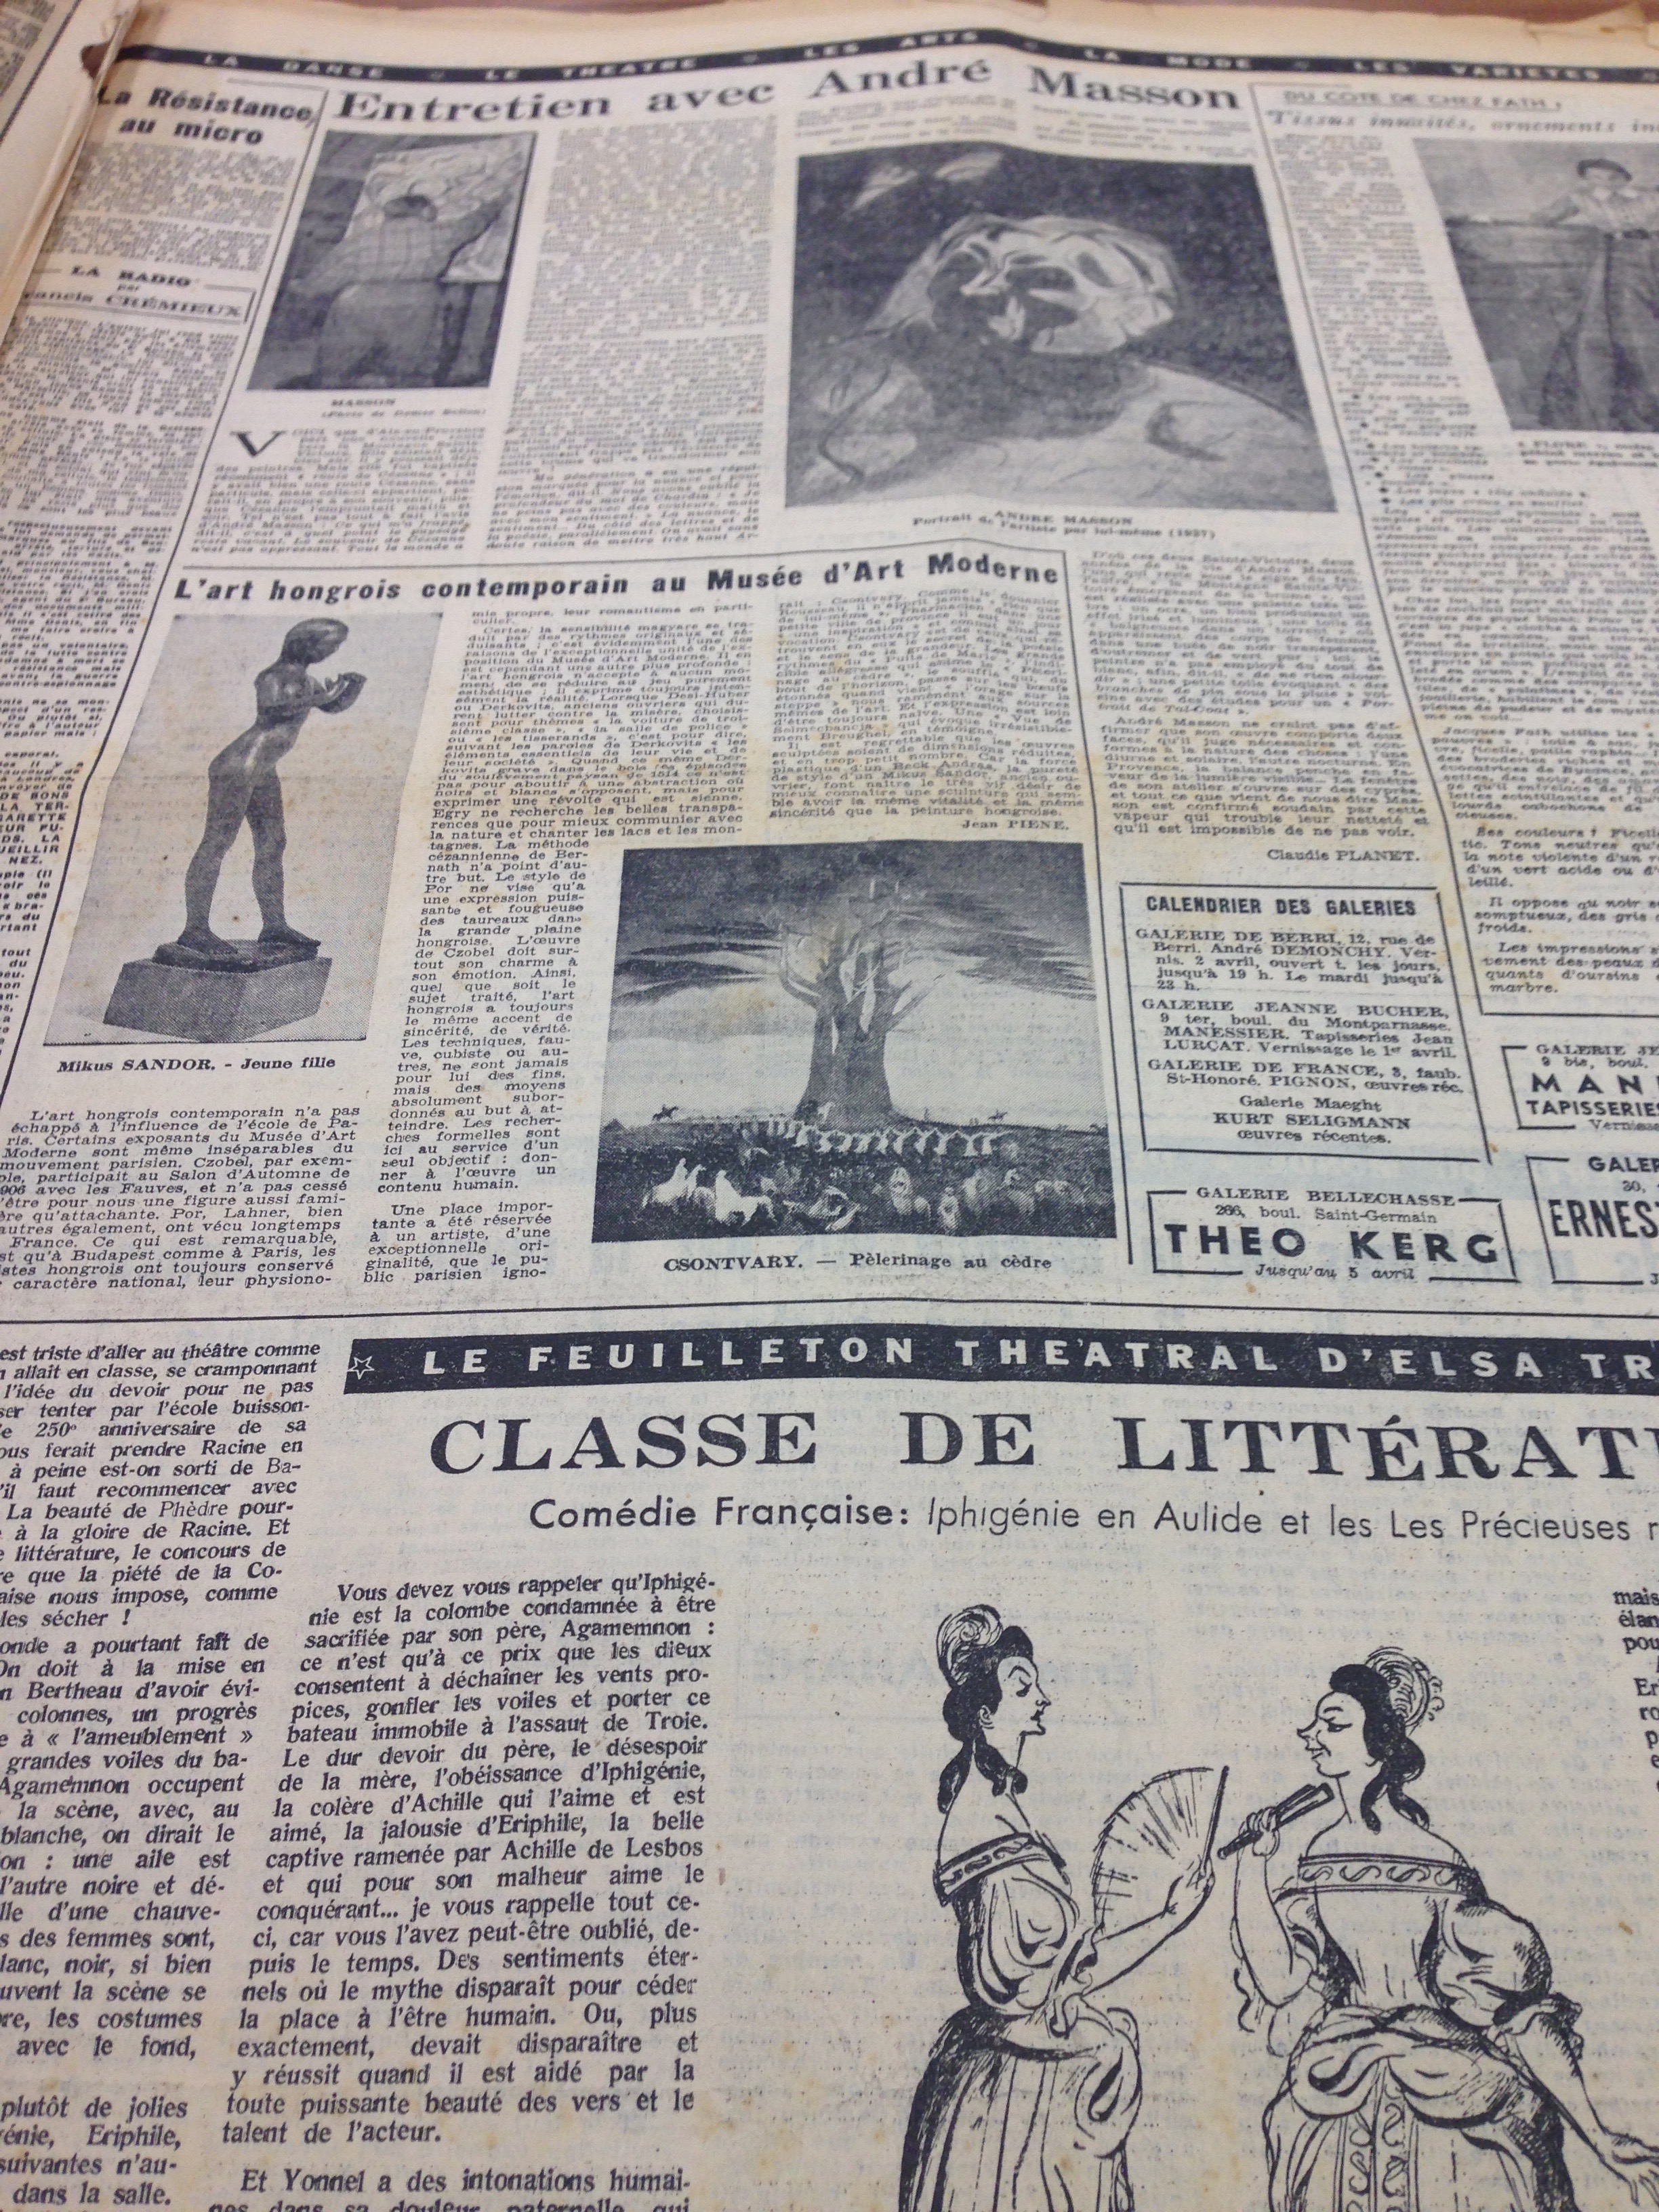
\includegraphics[width=\textwidth,height=\textheight,keepaspectratio]{Annexe/Image9.jpg}
	\caption{\cite{entretienmasson}}\label{fig:masson}
    \end{figure*}

    \begin{figure*}[htp]
   \centering
   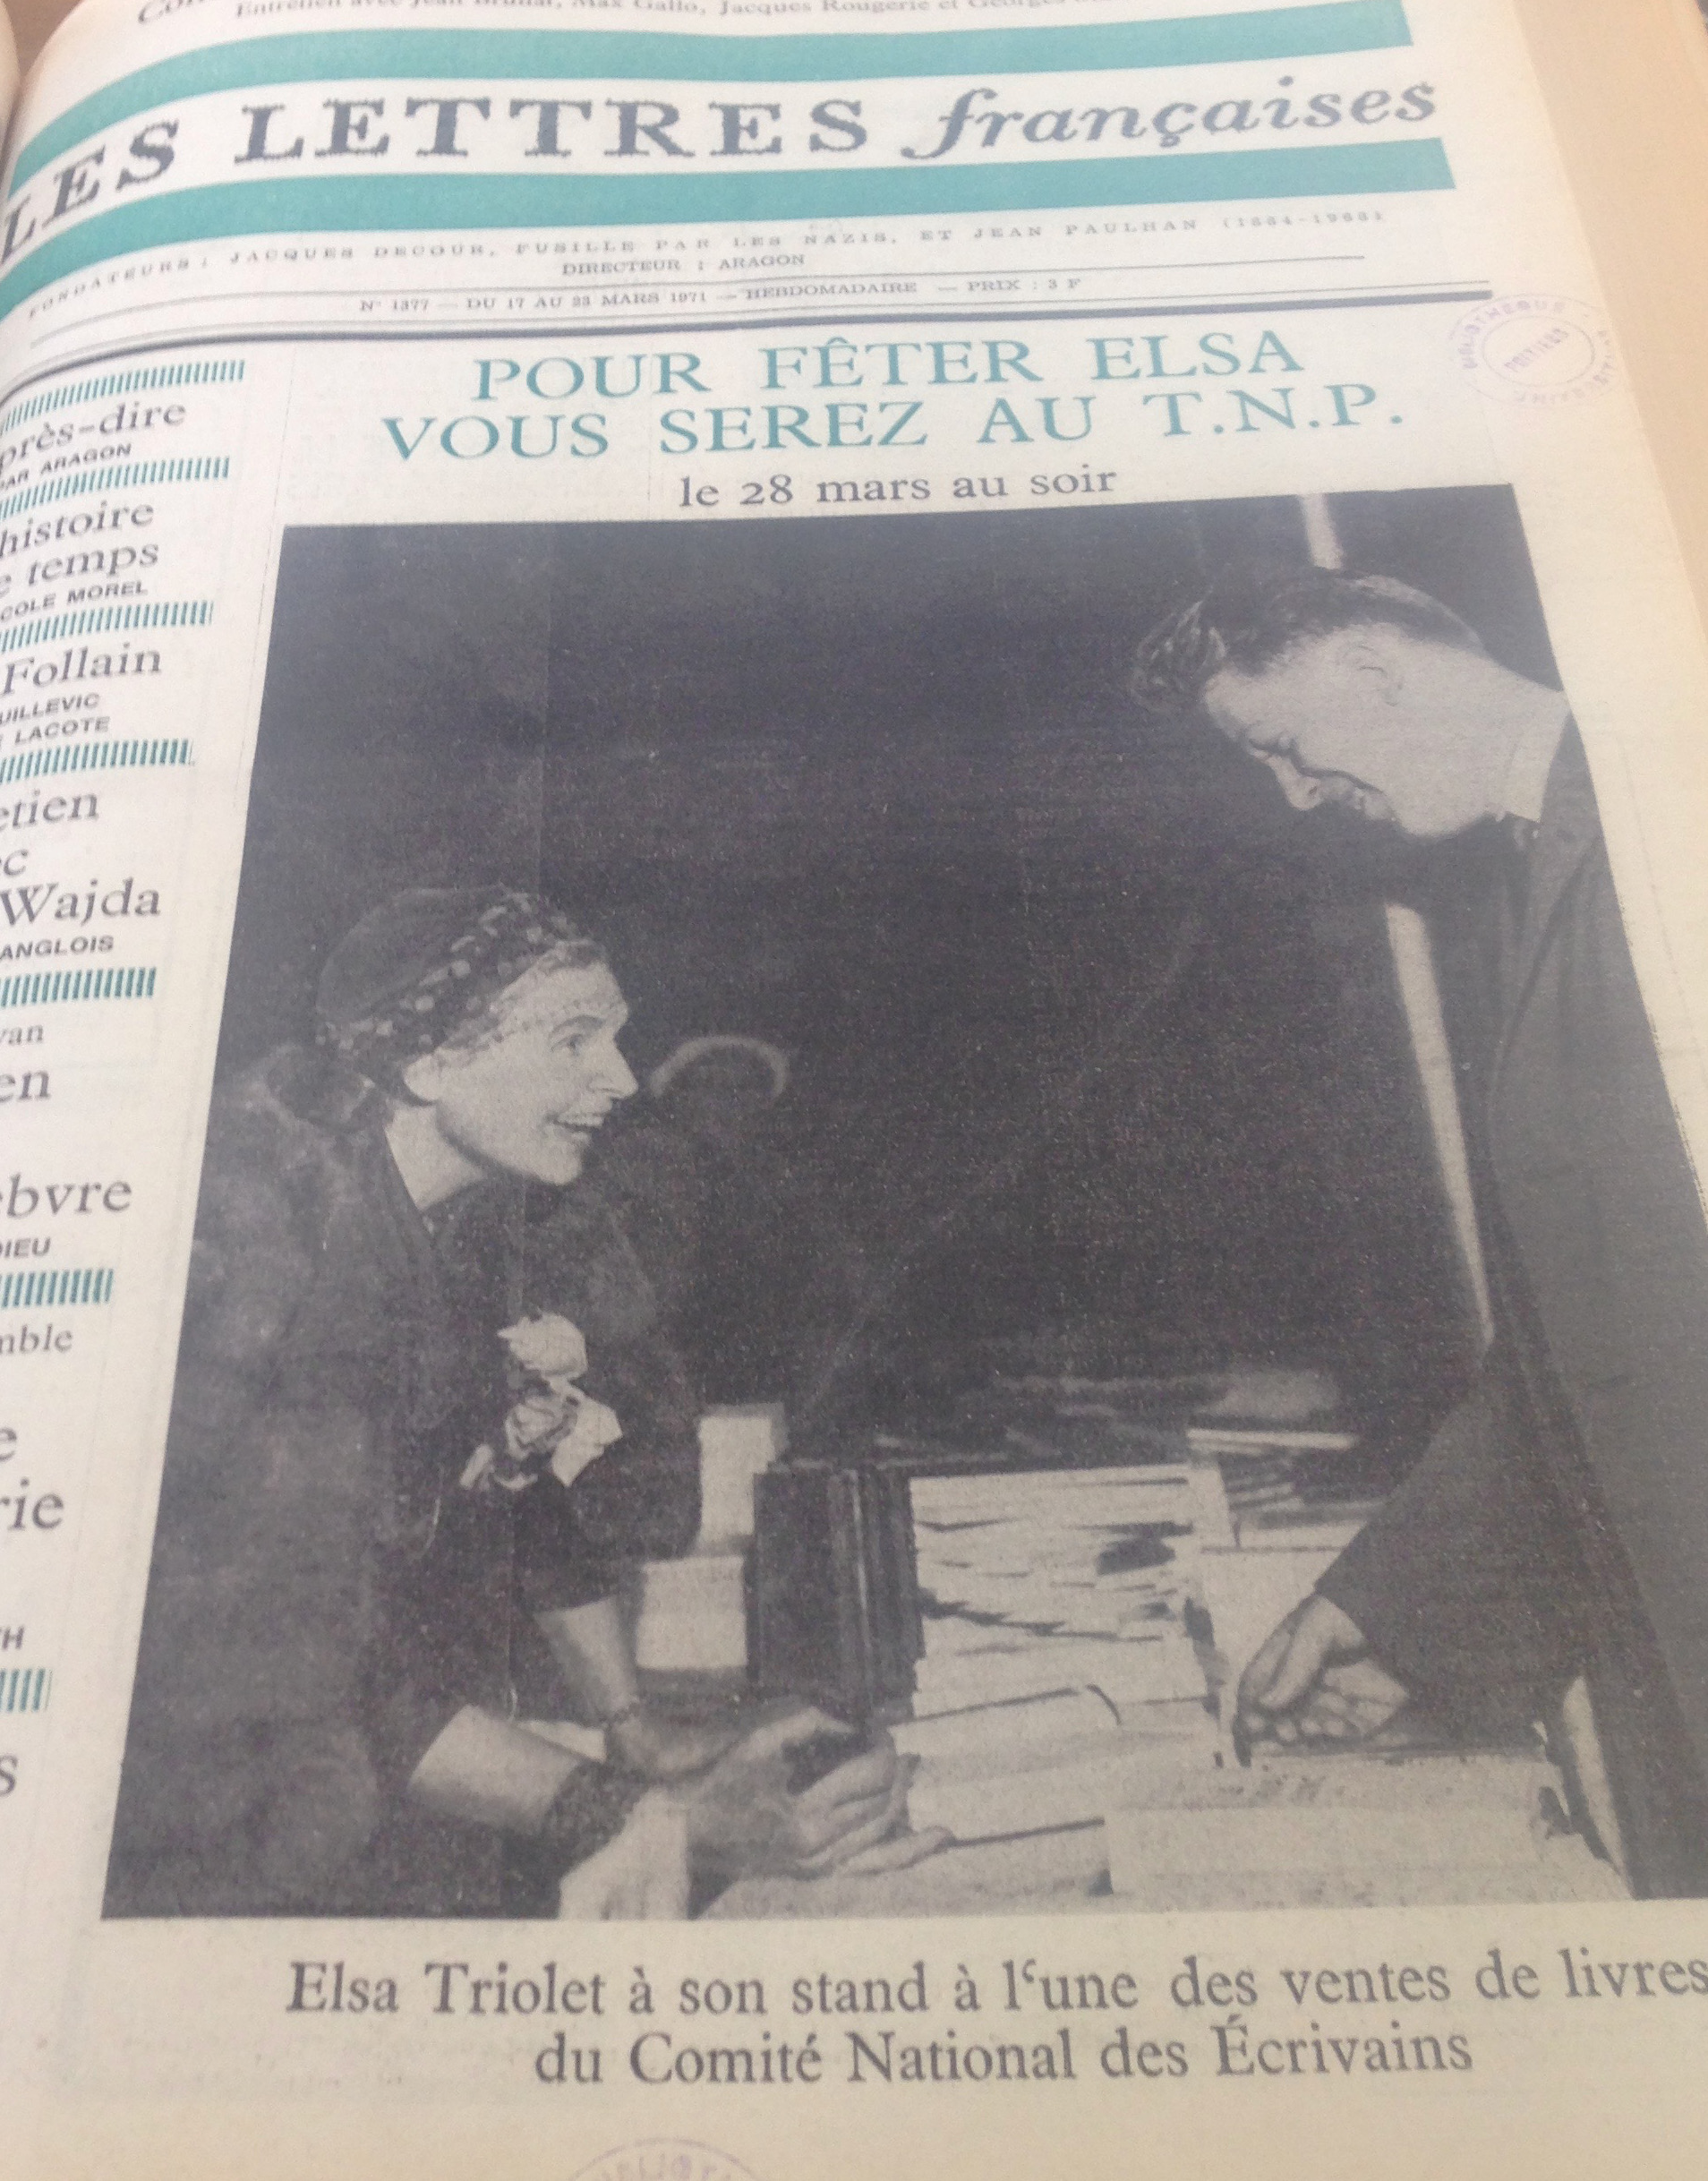
\includegraphics[width=\textwidth,height=\textheight,keepaspectratio]{Annexe/Image18.jpg}
	\caption{\cite{specialelsa}}\label{fig:elsa6}
    \end{figure*}

    \begin{figure*}[htp]
   \centering
   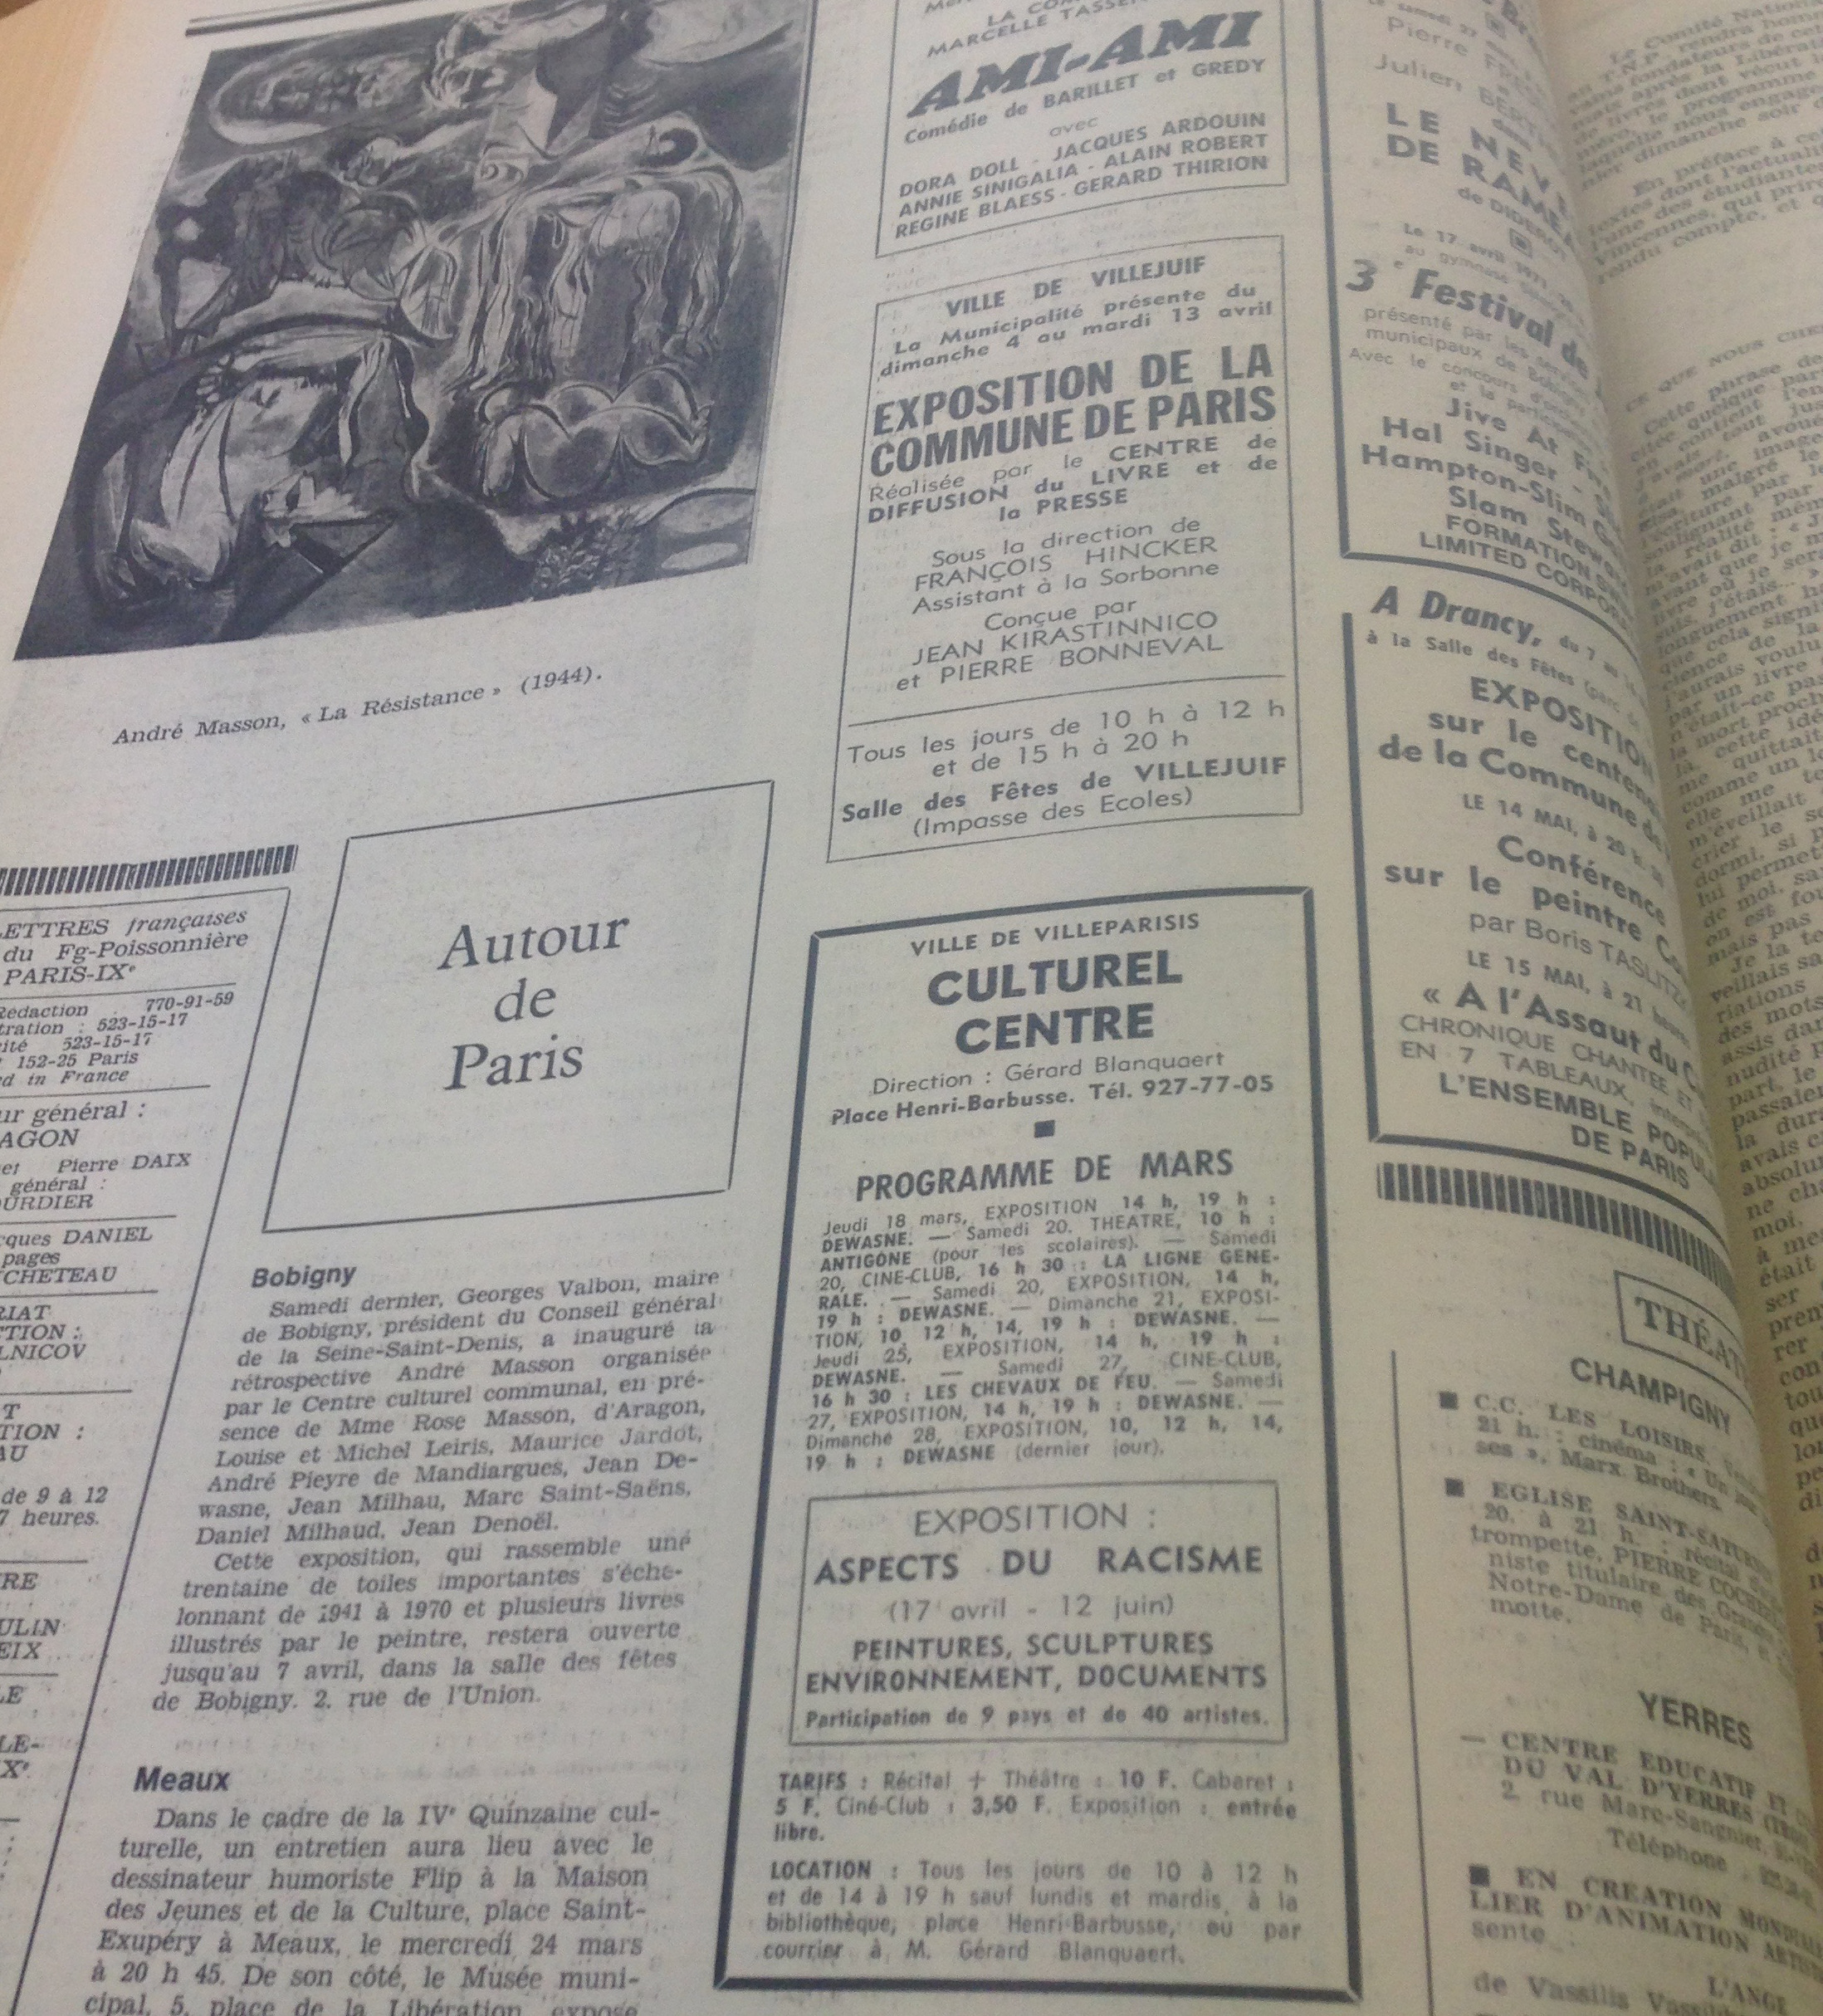
\includegraphics[width=\textwidth,height=\textheight,keepaspectratio]{Annexe/Image33.jpg}
	\caption{\cite{specialelsa}}\label{fig:elsa8}
    \end{figure*}


    \begin{figure*}[htp]
   \centering
   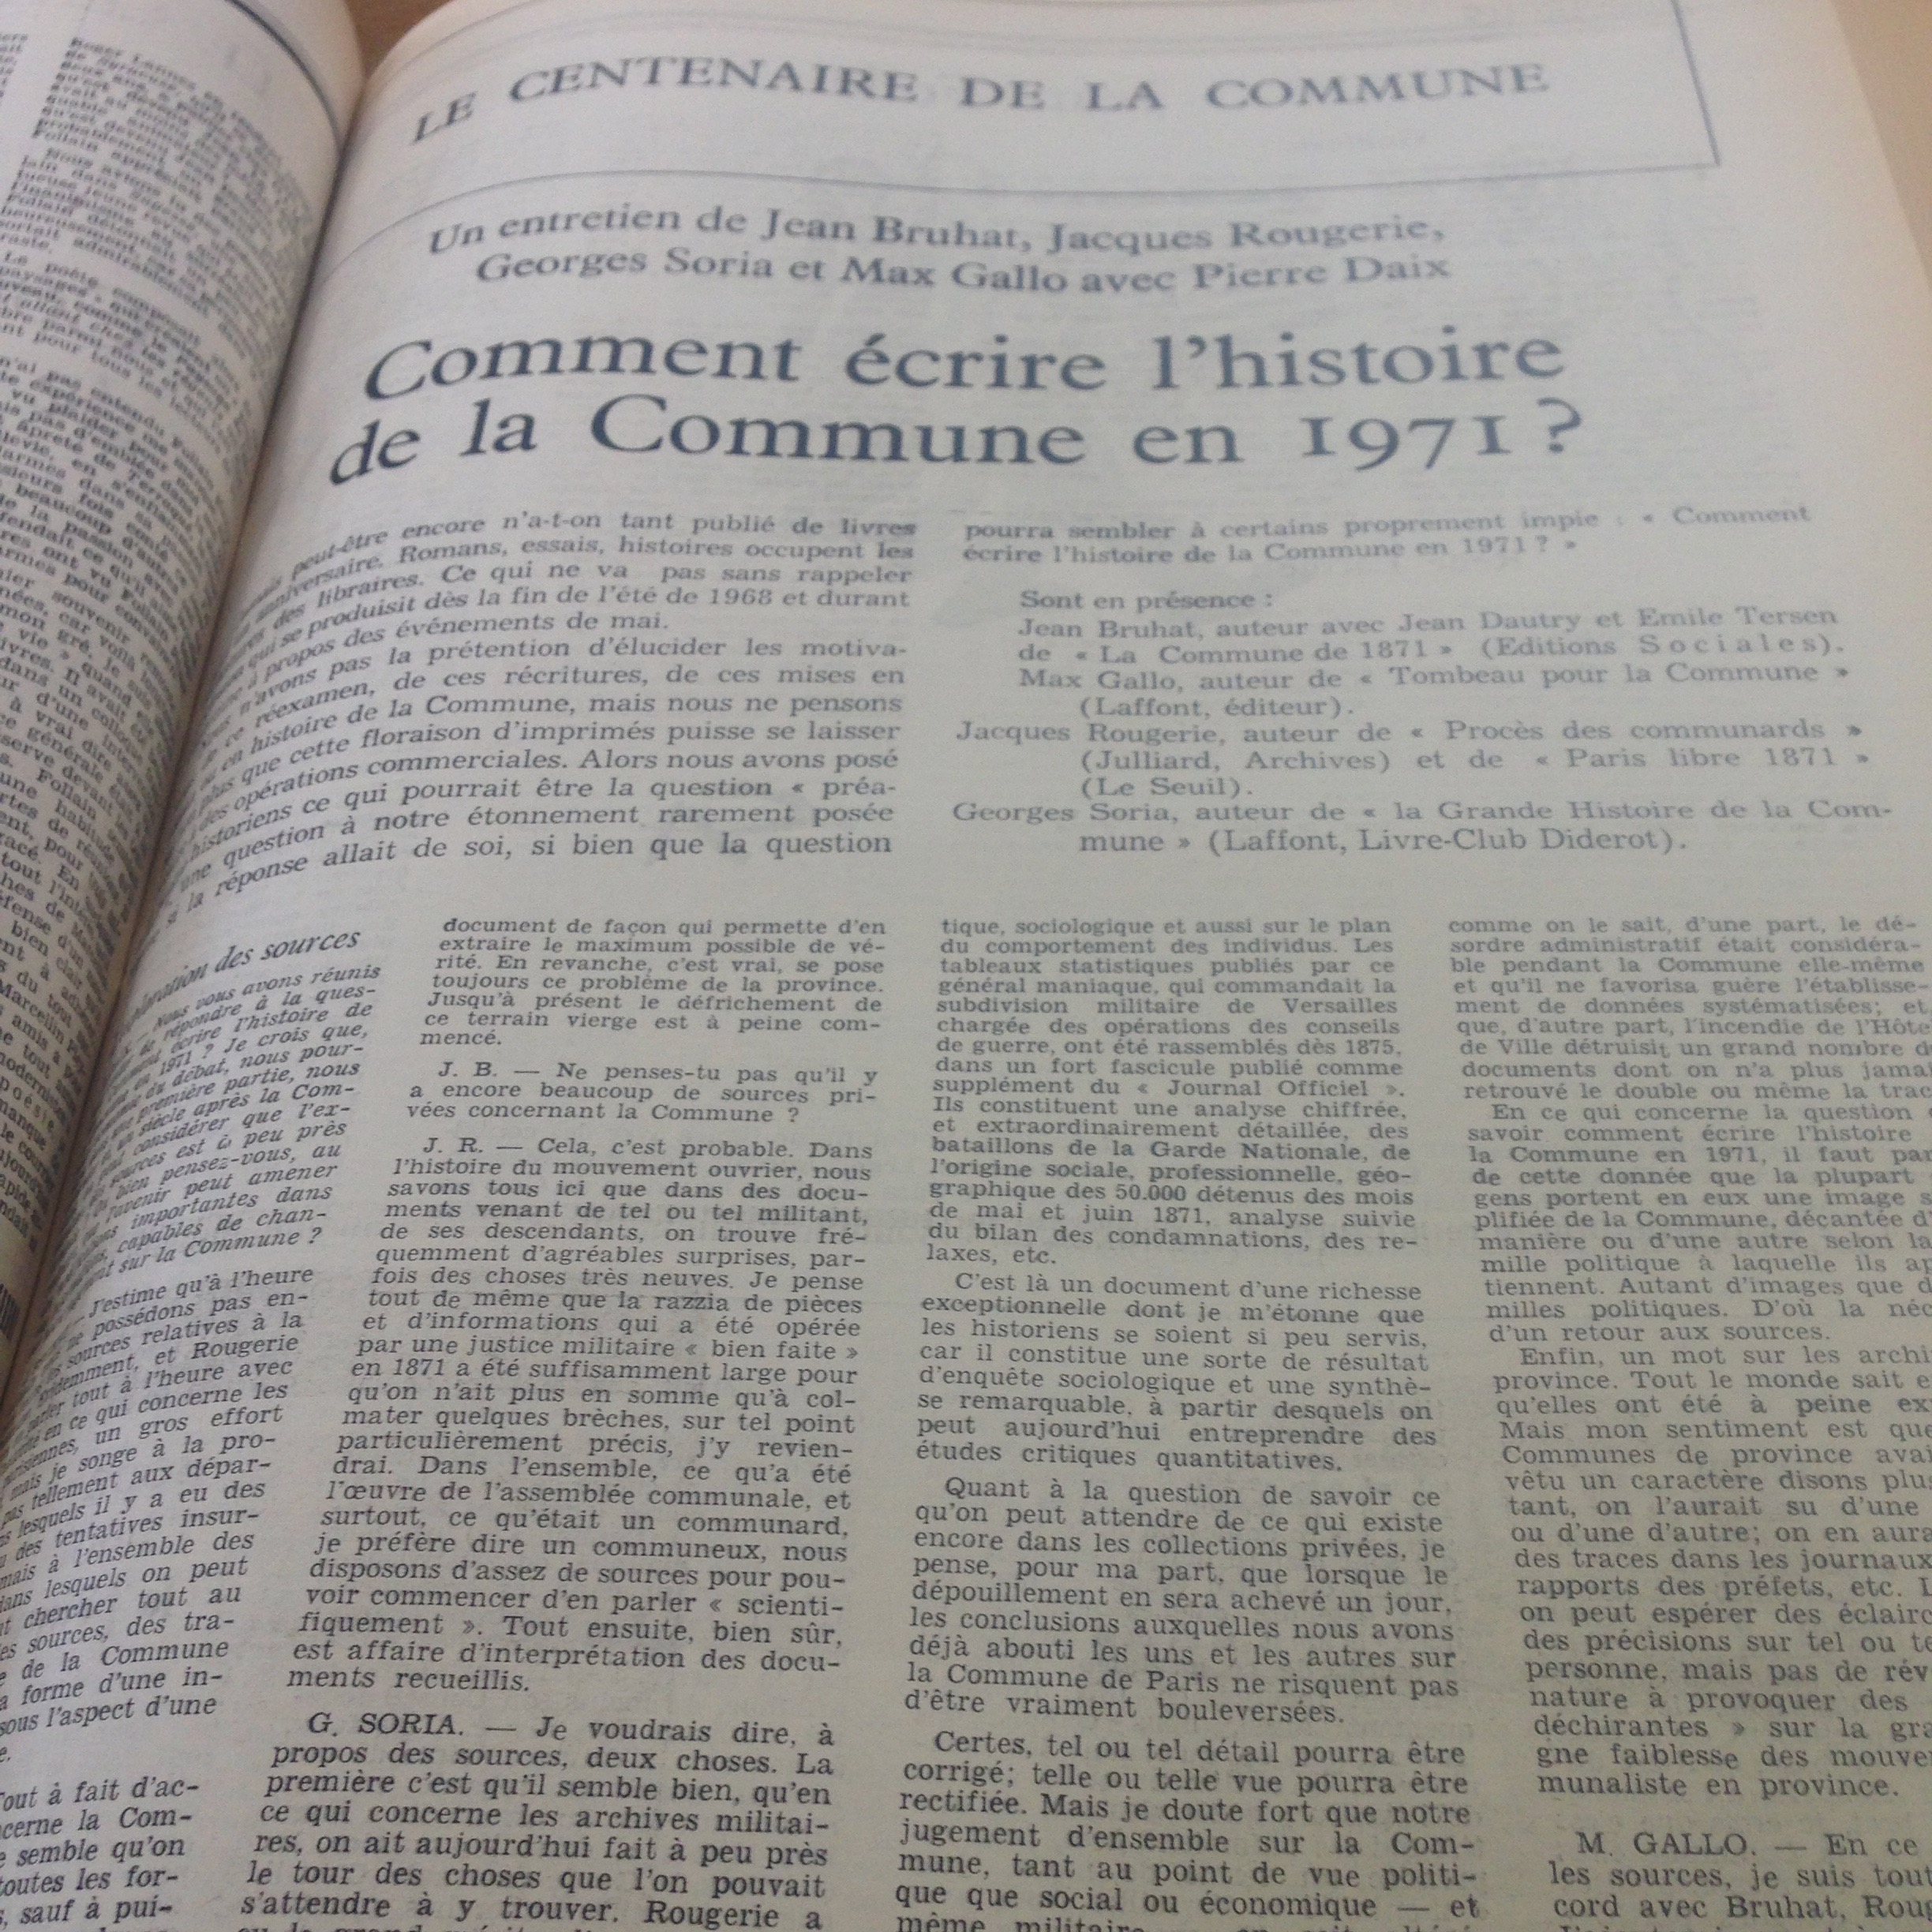
\includegraphics[width=\textwidth,height=\textheight,keepaspectratio]{Annexe/Image19.jpg}
	\caption{\cite{specialelsa}}\label{fig:elsa7}
    \end{figure*}
    

    \begin{figure*}[htp]
   \centering
   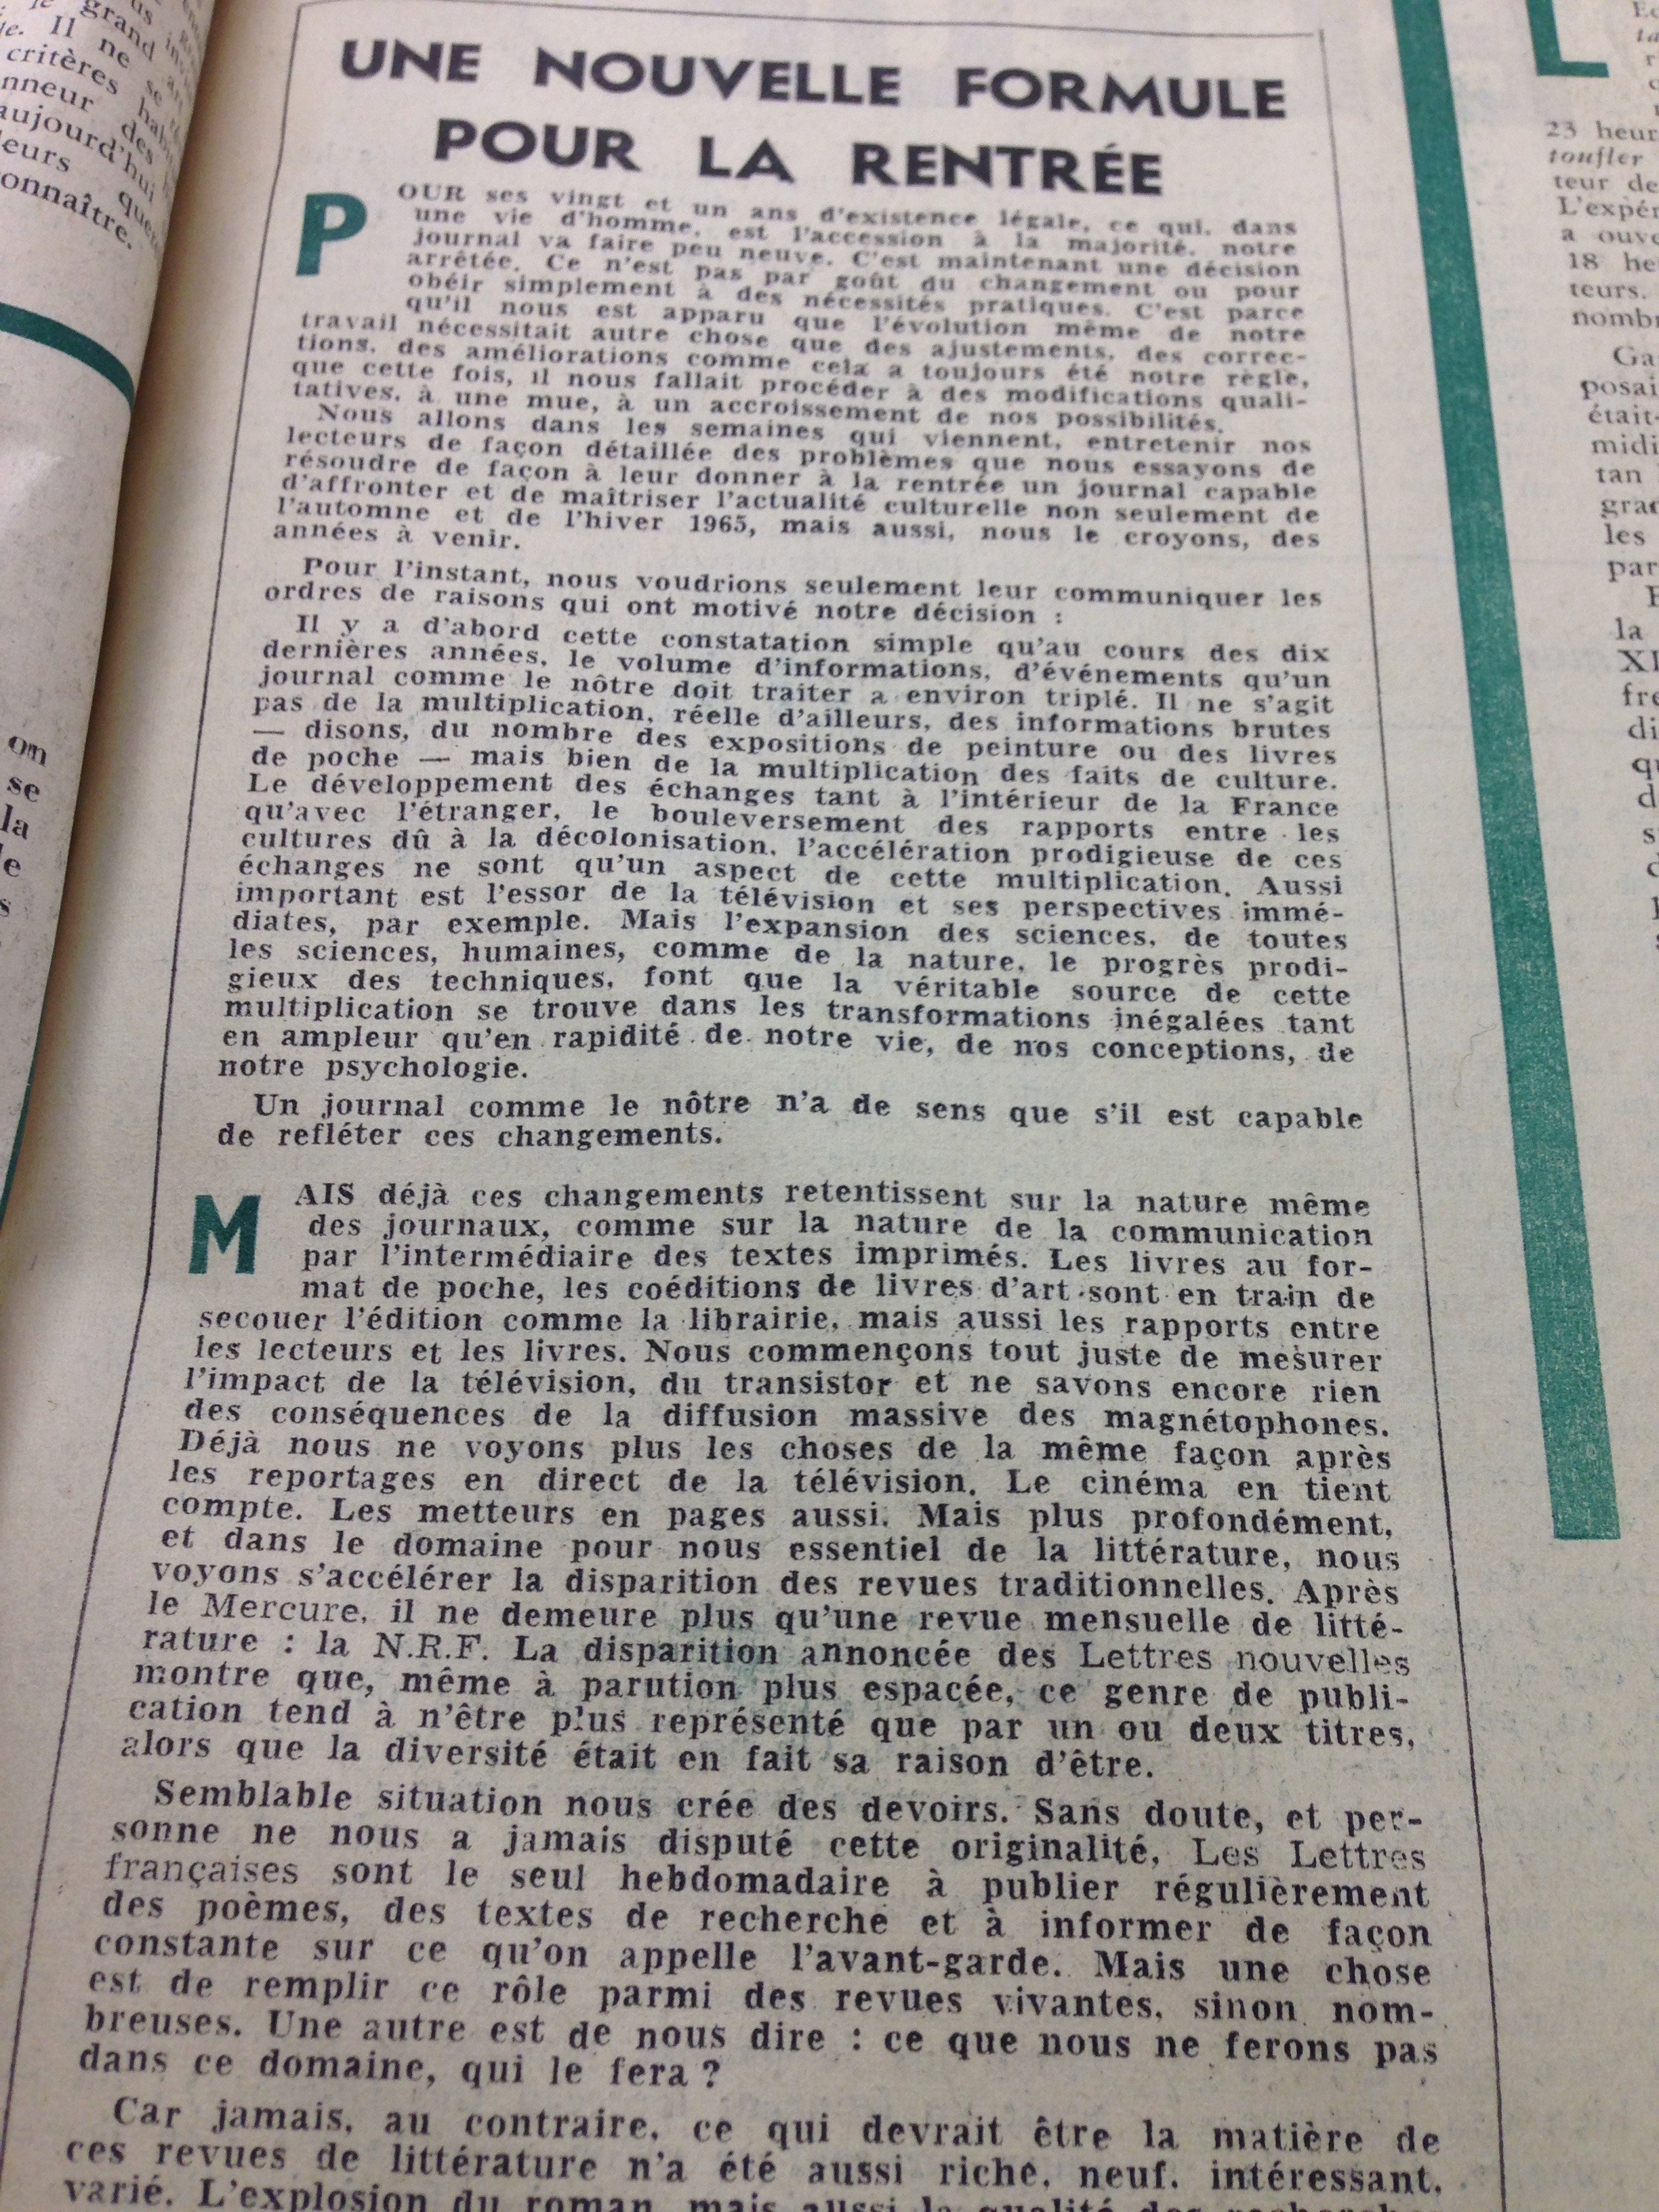
\includegraphics[width=\textwidth,height=\textheight,keepaspectratio]{Annexe/Image22.jpg}
	\caption{\cite{nouvelleformule}}\label{fig:formule2}
    \end{figure*}


 \begin{figure*}[htp]
   \centering
   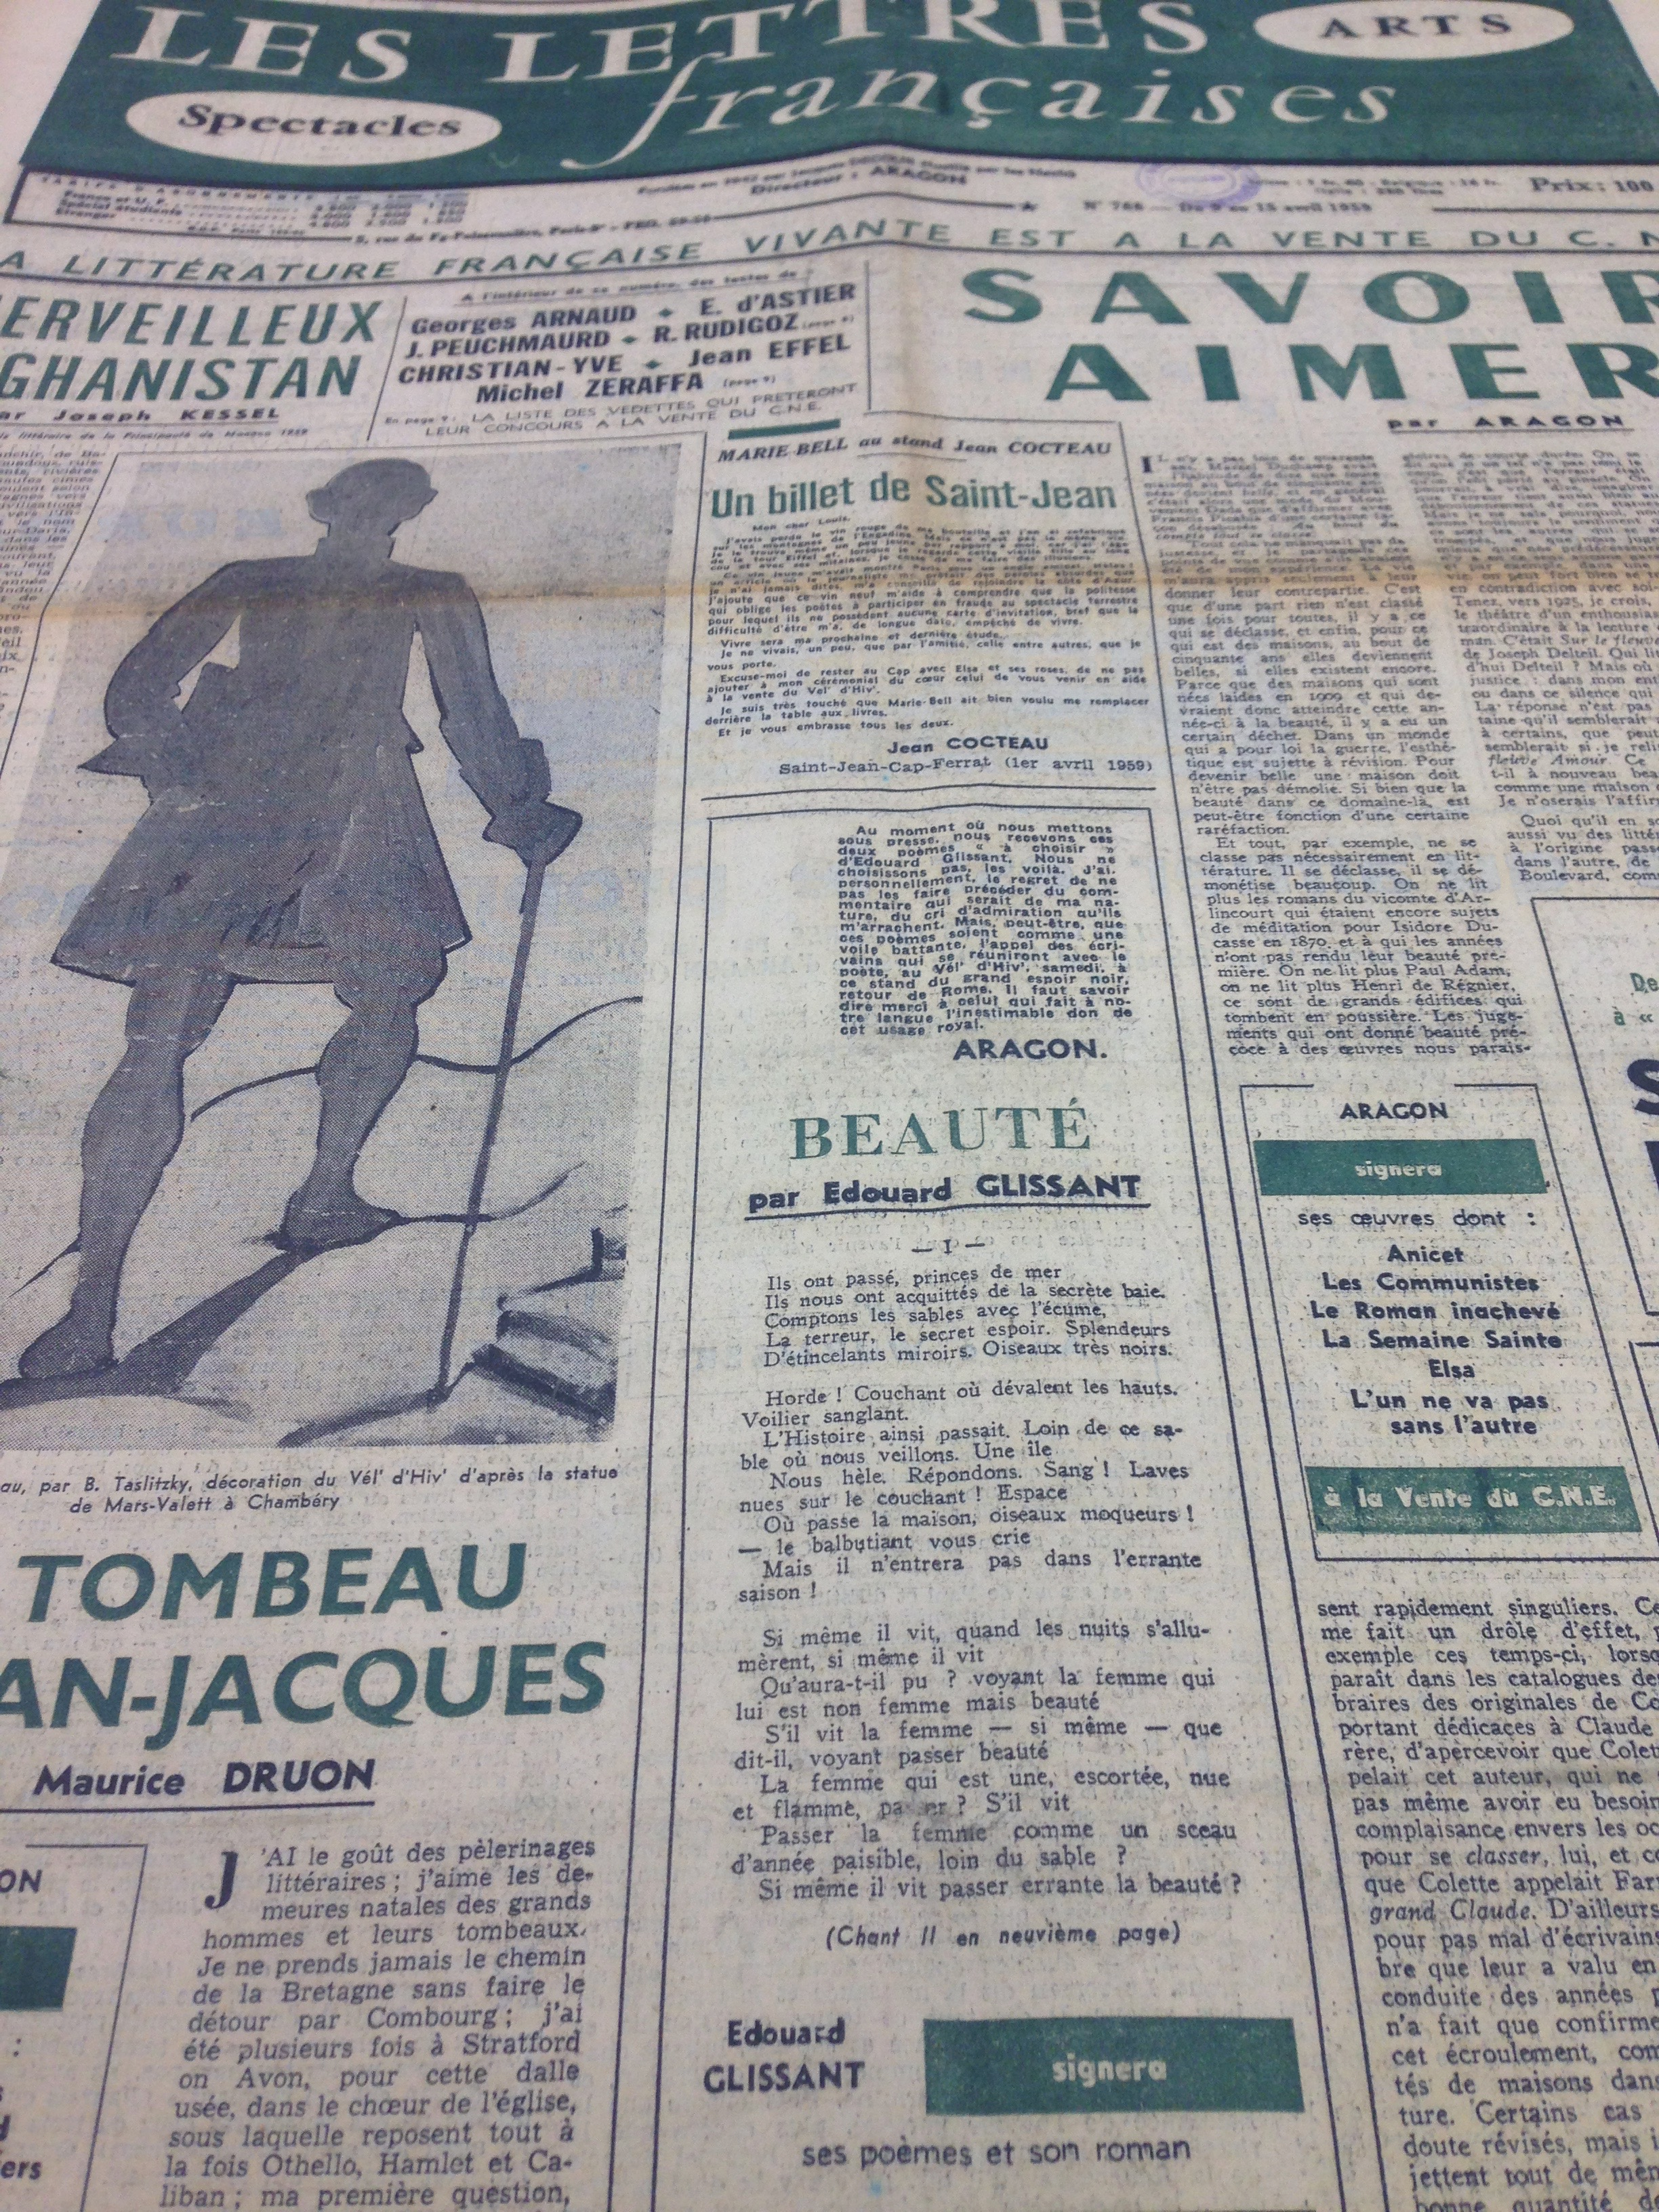
\includegraphics[width=\textwidth,height=\textheight,keepaspectratio]{Annexe/Image32.jpg}
	\caption{\cite{savoiraimer}}\label{fig:savoiraimer}
    \end{figure*}


    \begin{figure*}[htp]
   \centering
   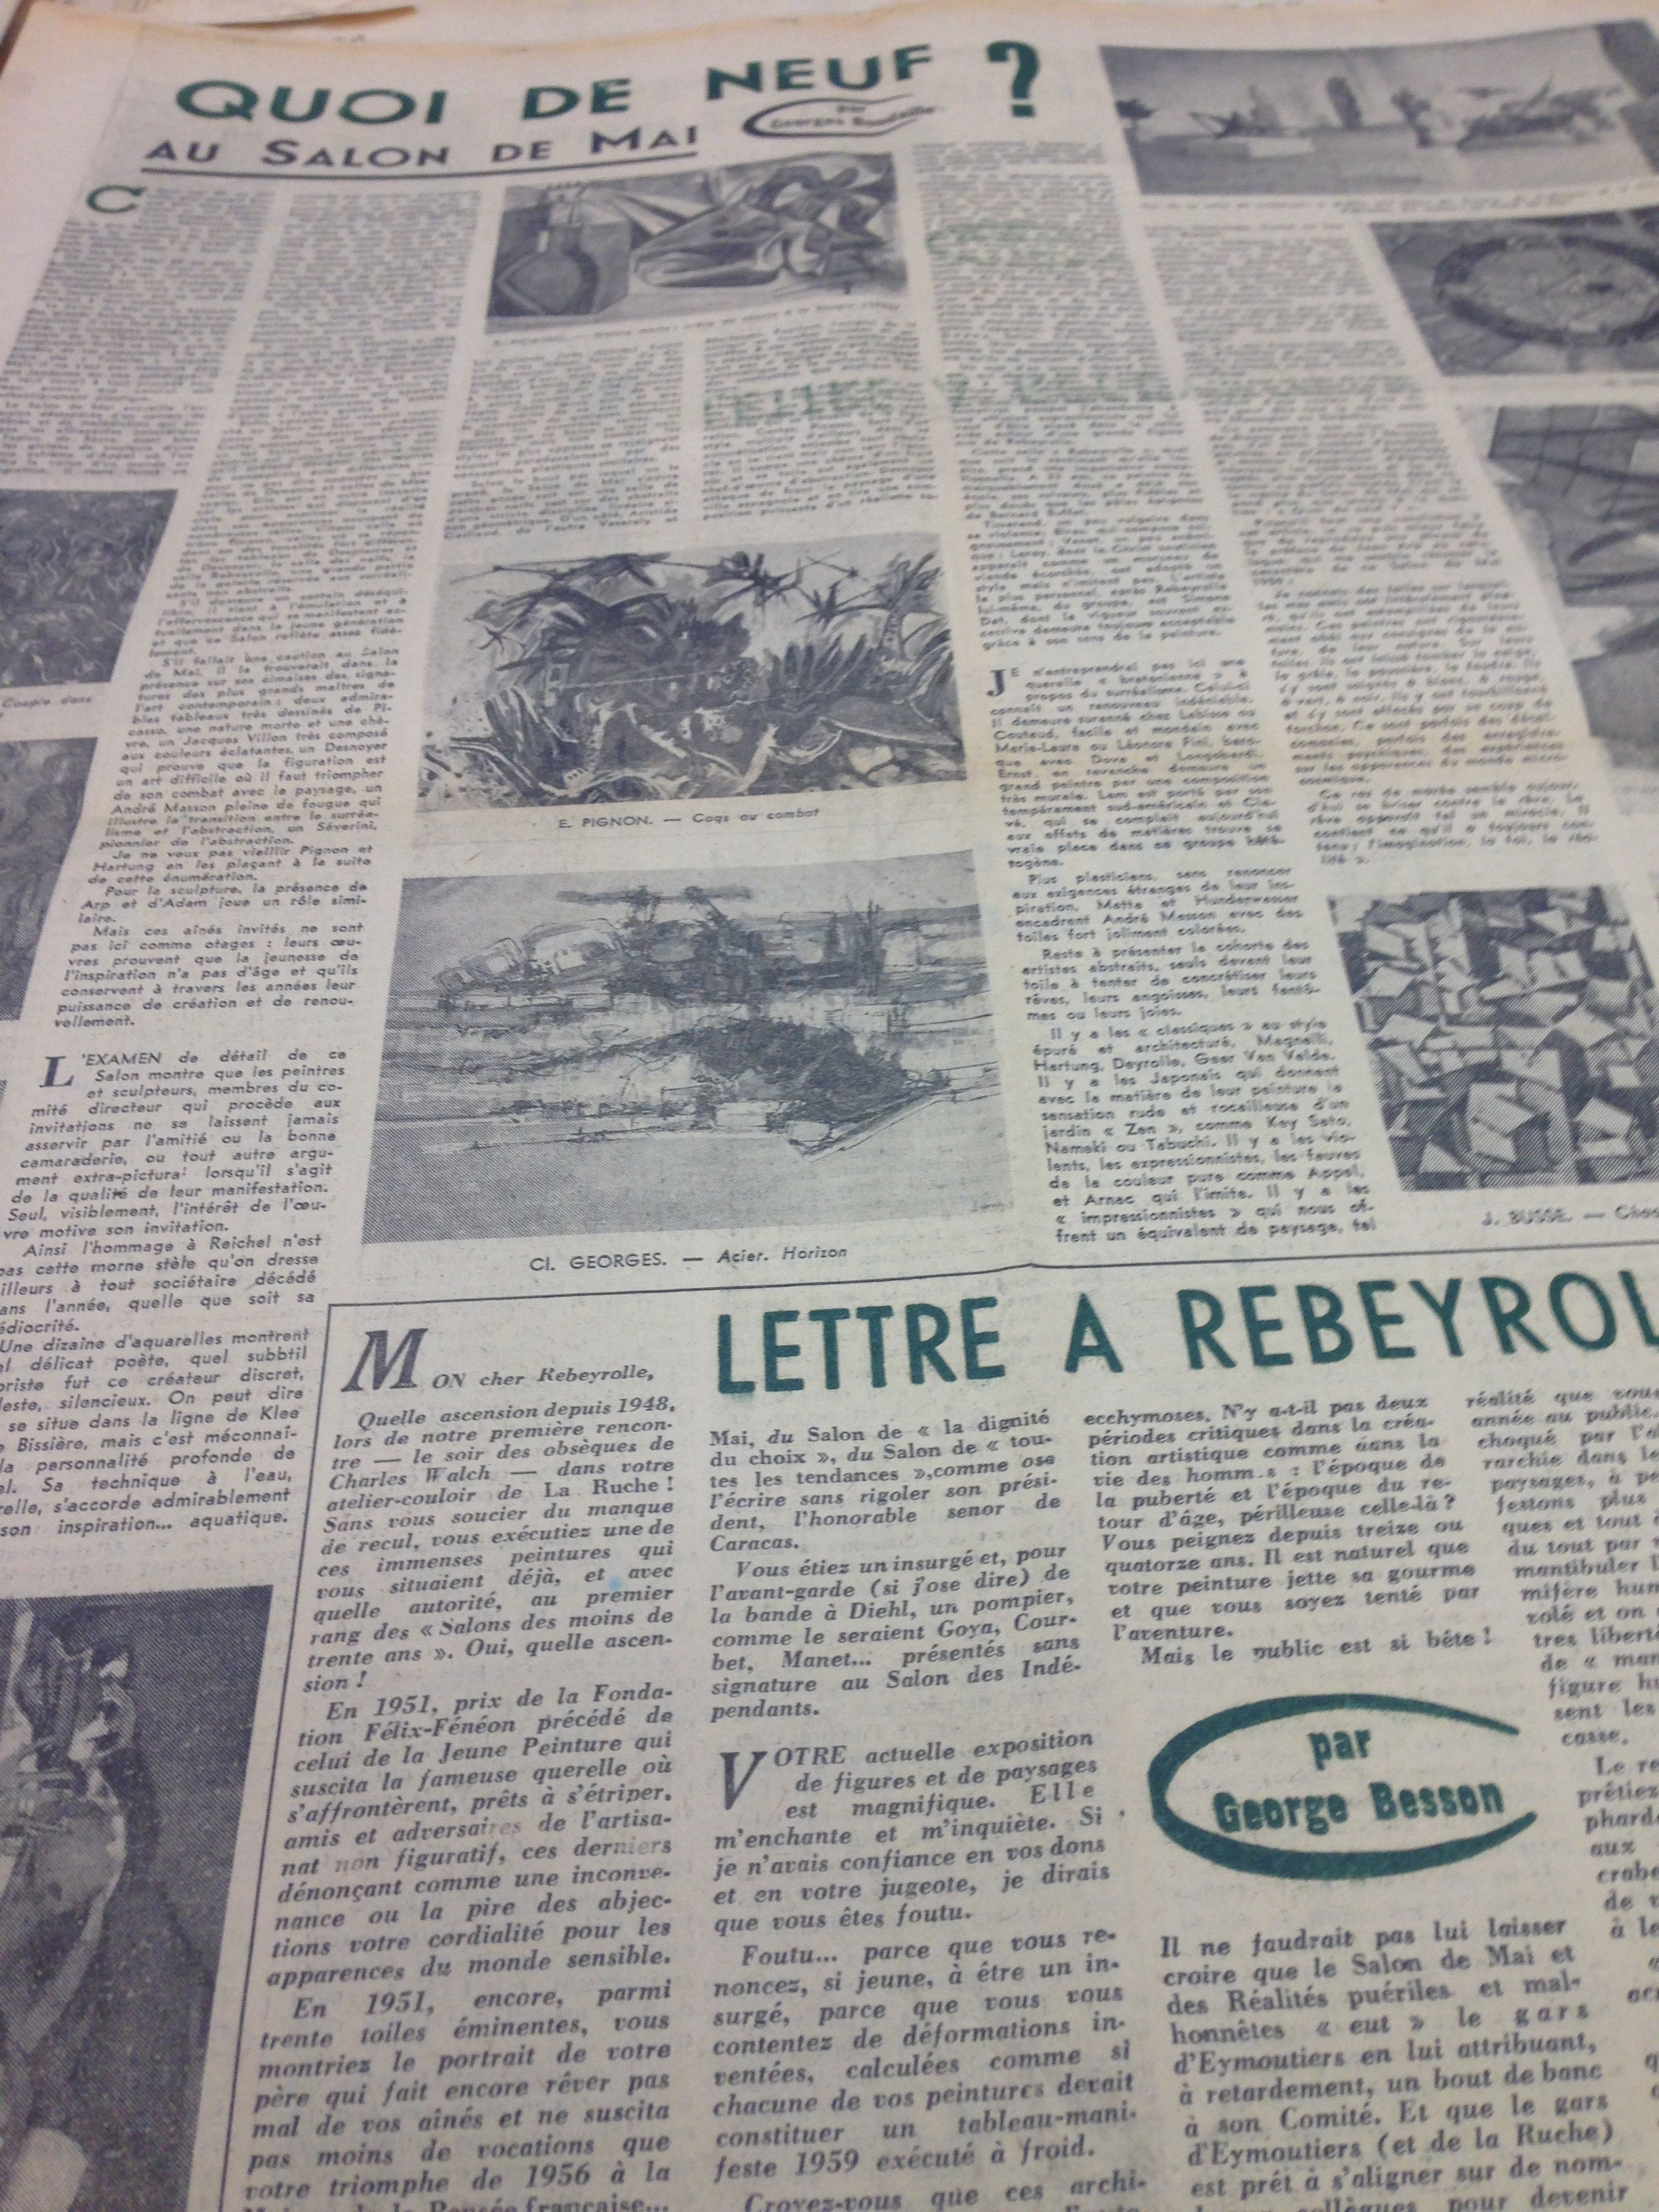
\includegraphics[width=\textwidth,height=\textheight,keepaspectratio]{Annexe/Image31.jpg}
	\caption{\cite{salondemai}}\label{fig:salondemai}
    \end{figure*}


    \begin{figure*}[htp]
   \centering
   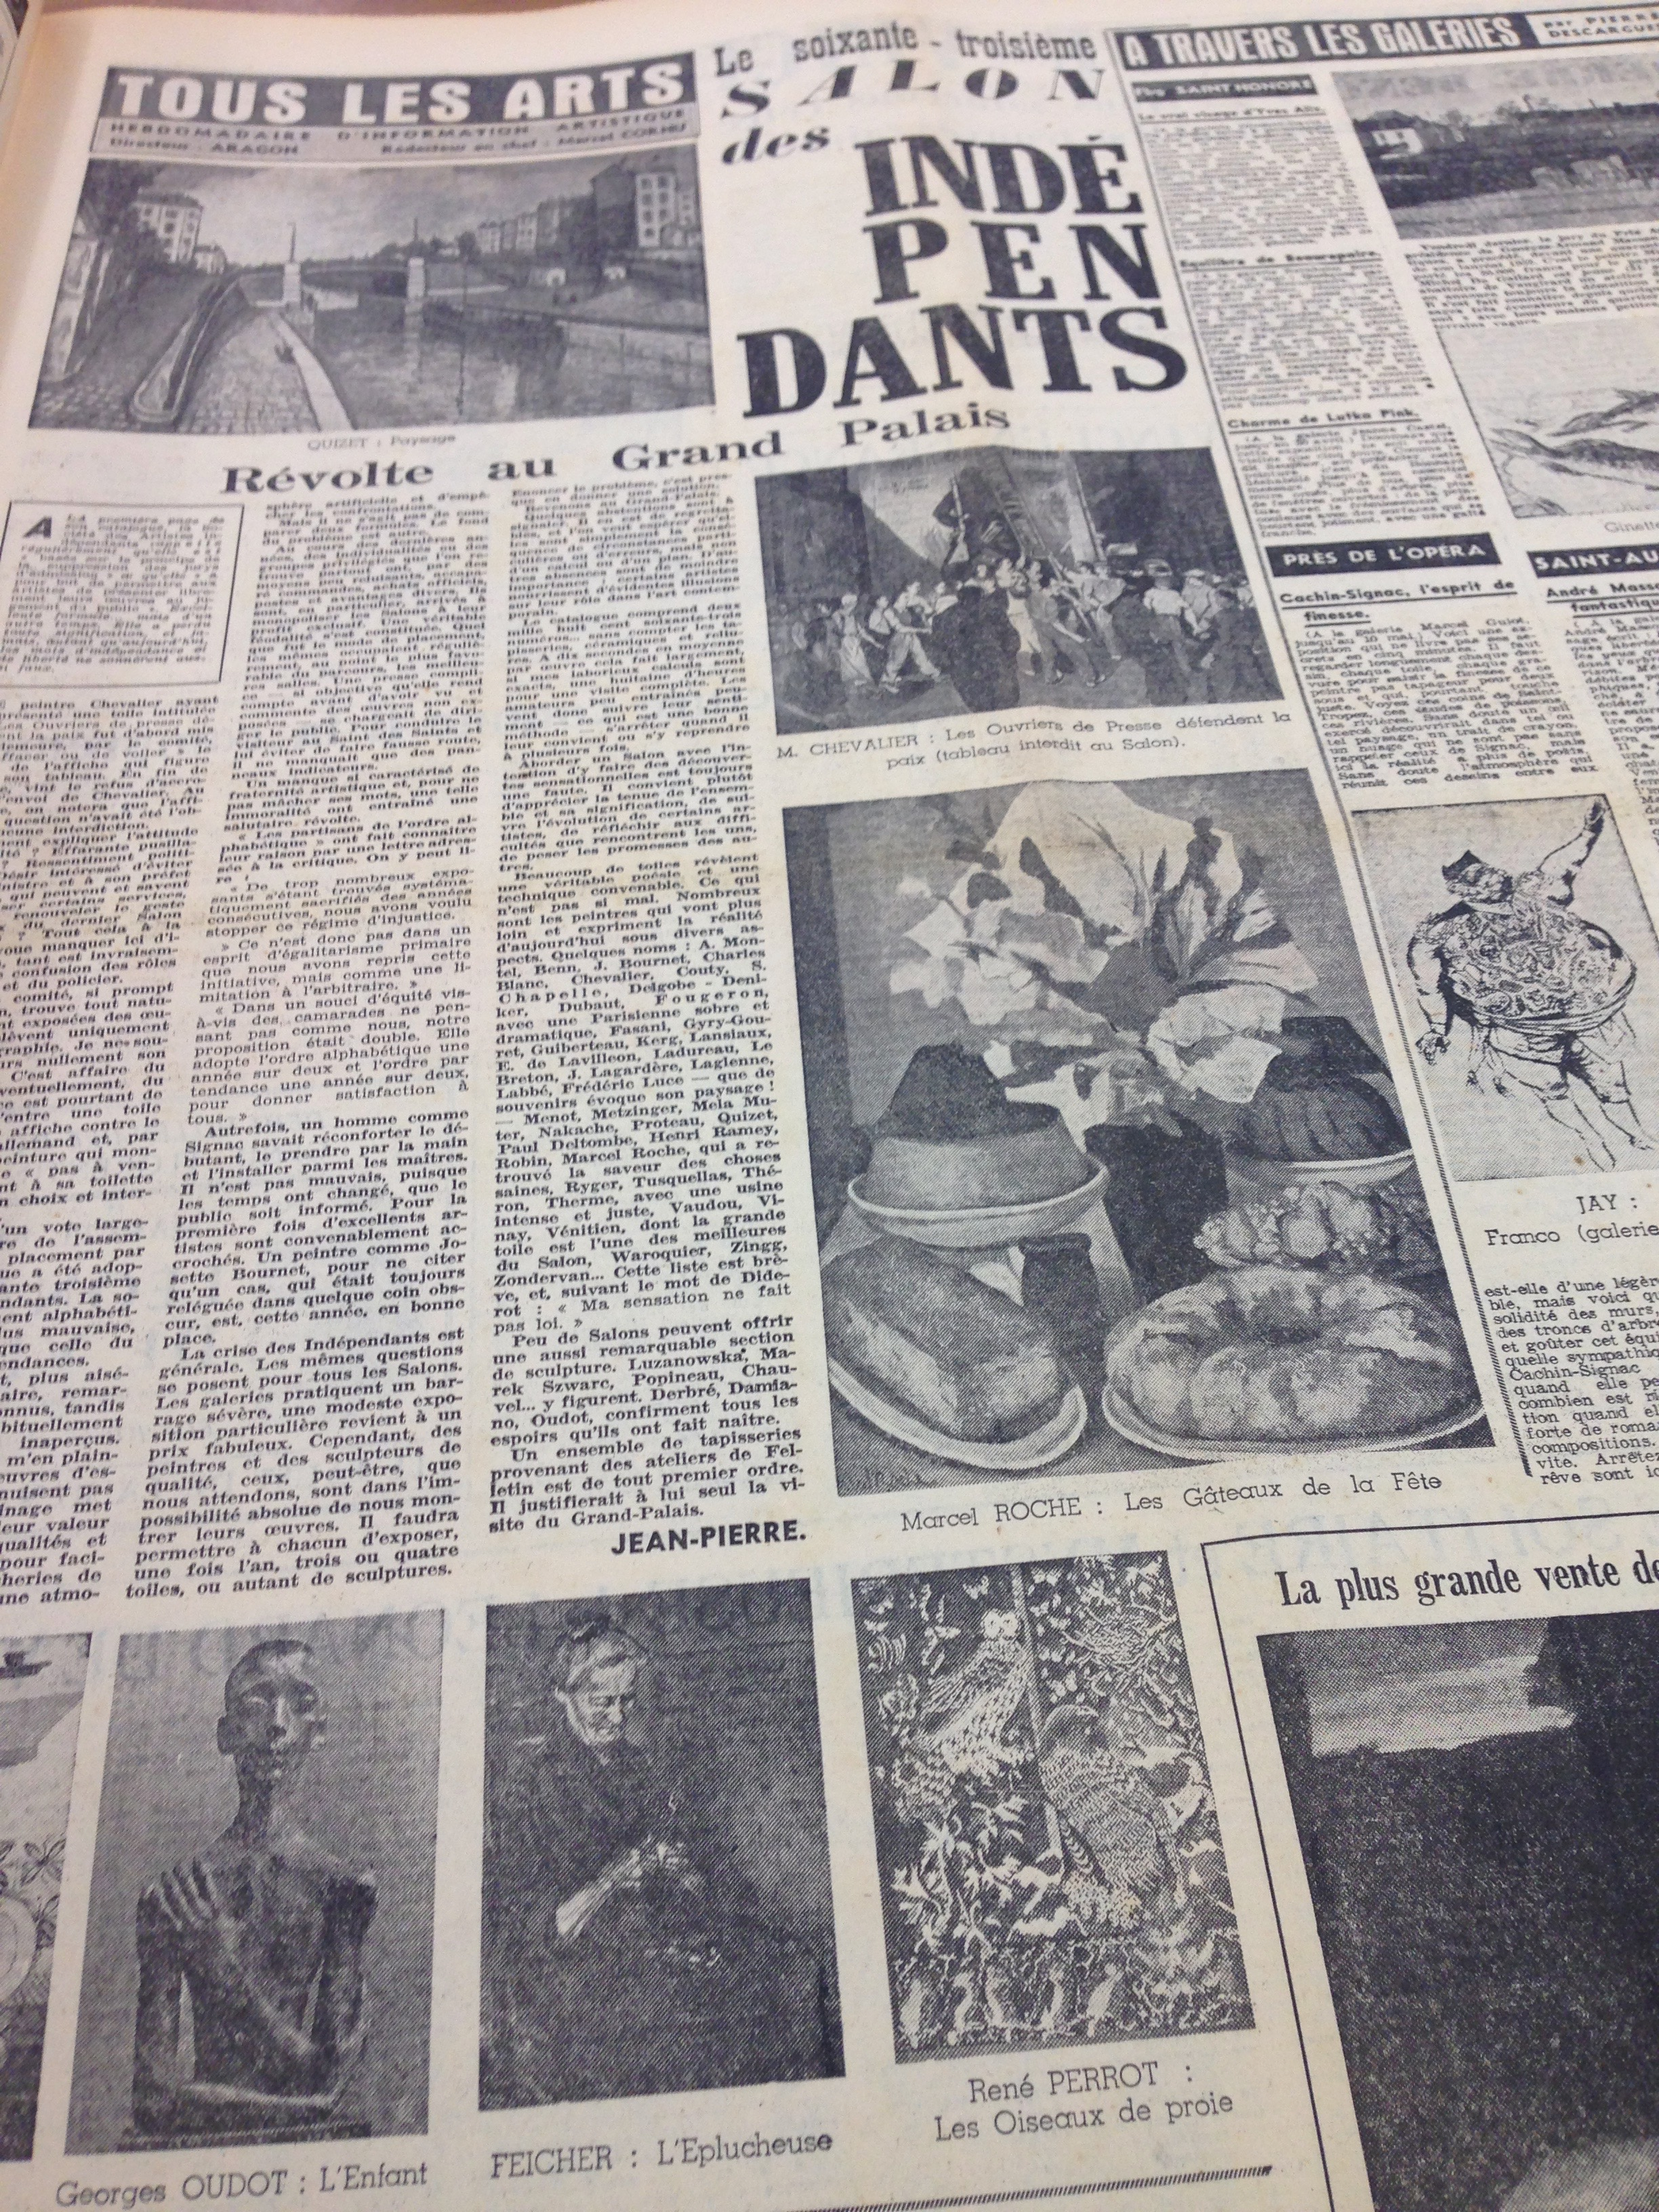
\includegraphics[width=\textwidth,height=\textheight,keepaspectratio]{Annexe/Image24.jpg}
	\caption{\cite{reelfantastique}}\label{fig:reelfantastique}
    \end{figure*}

    \begin{figure*}[htp]
   \centering
   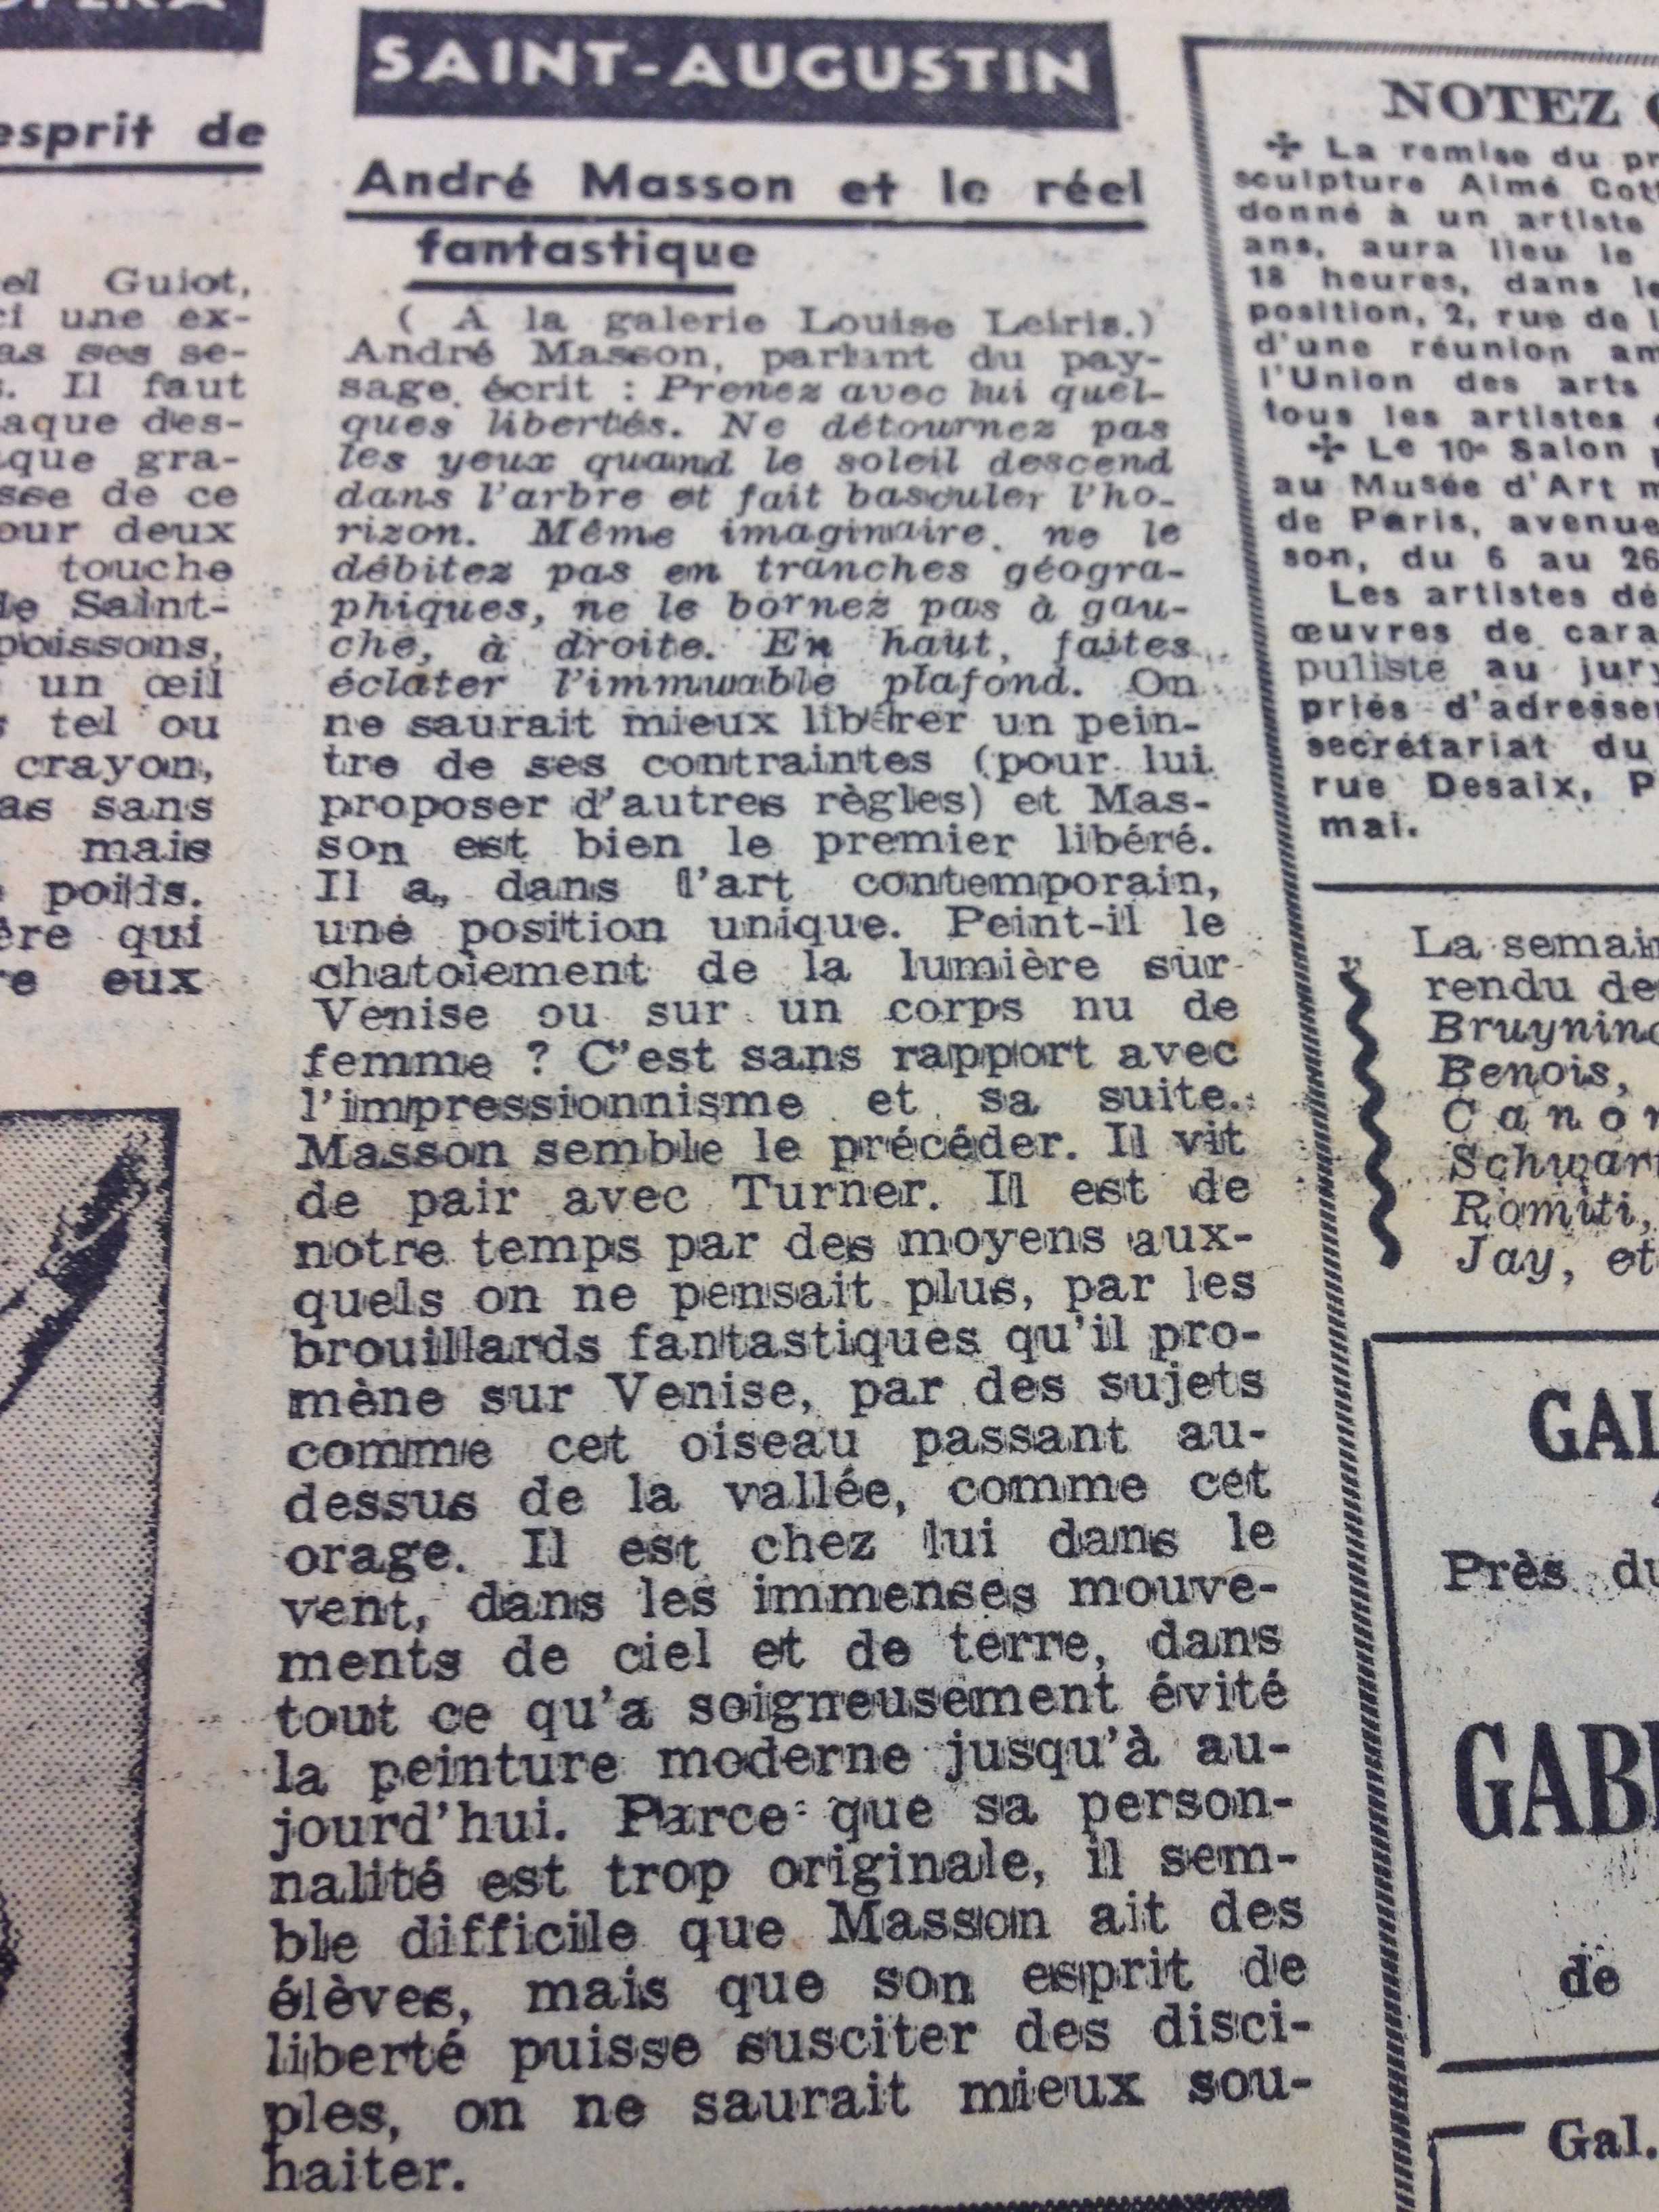
\includegraphics[width=\textwidth,height=\textheight,keepaspectratio]{Annexe/Image29.jpg}
	\caption{\cite{reelfantastique}}\label{fig:reelfantastique2}
    \end{figure*}

 \begin{figure*}[htp]
   \centering
   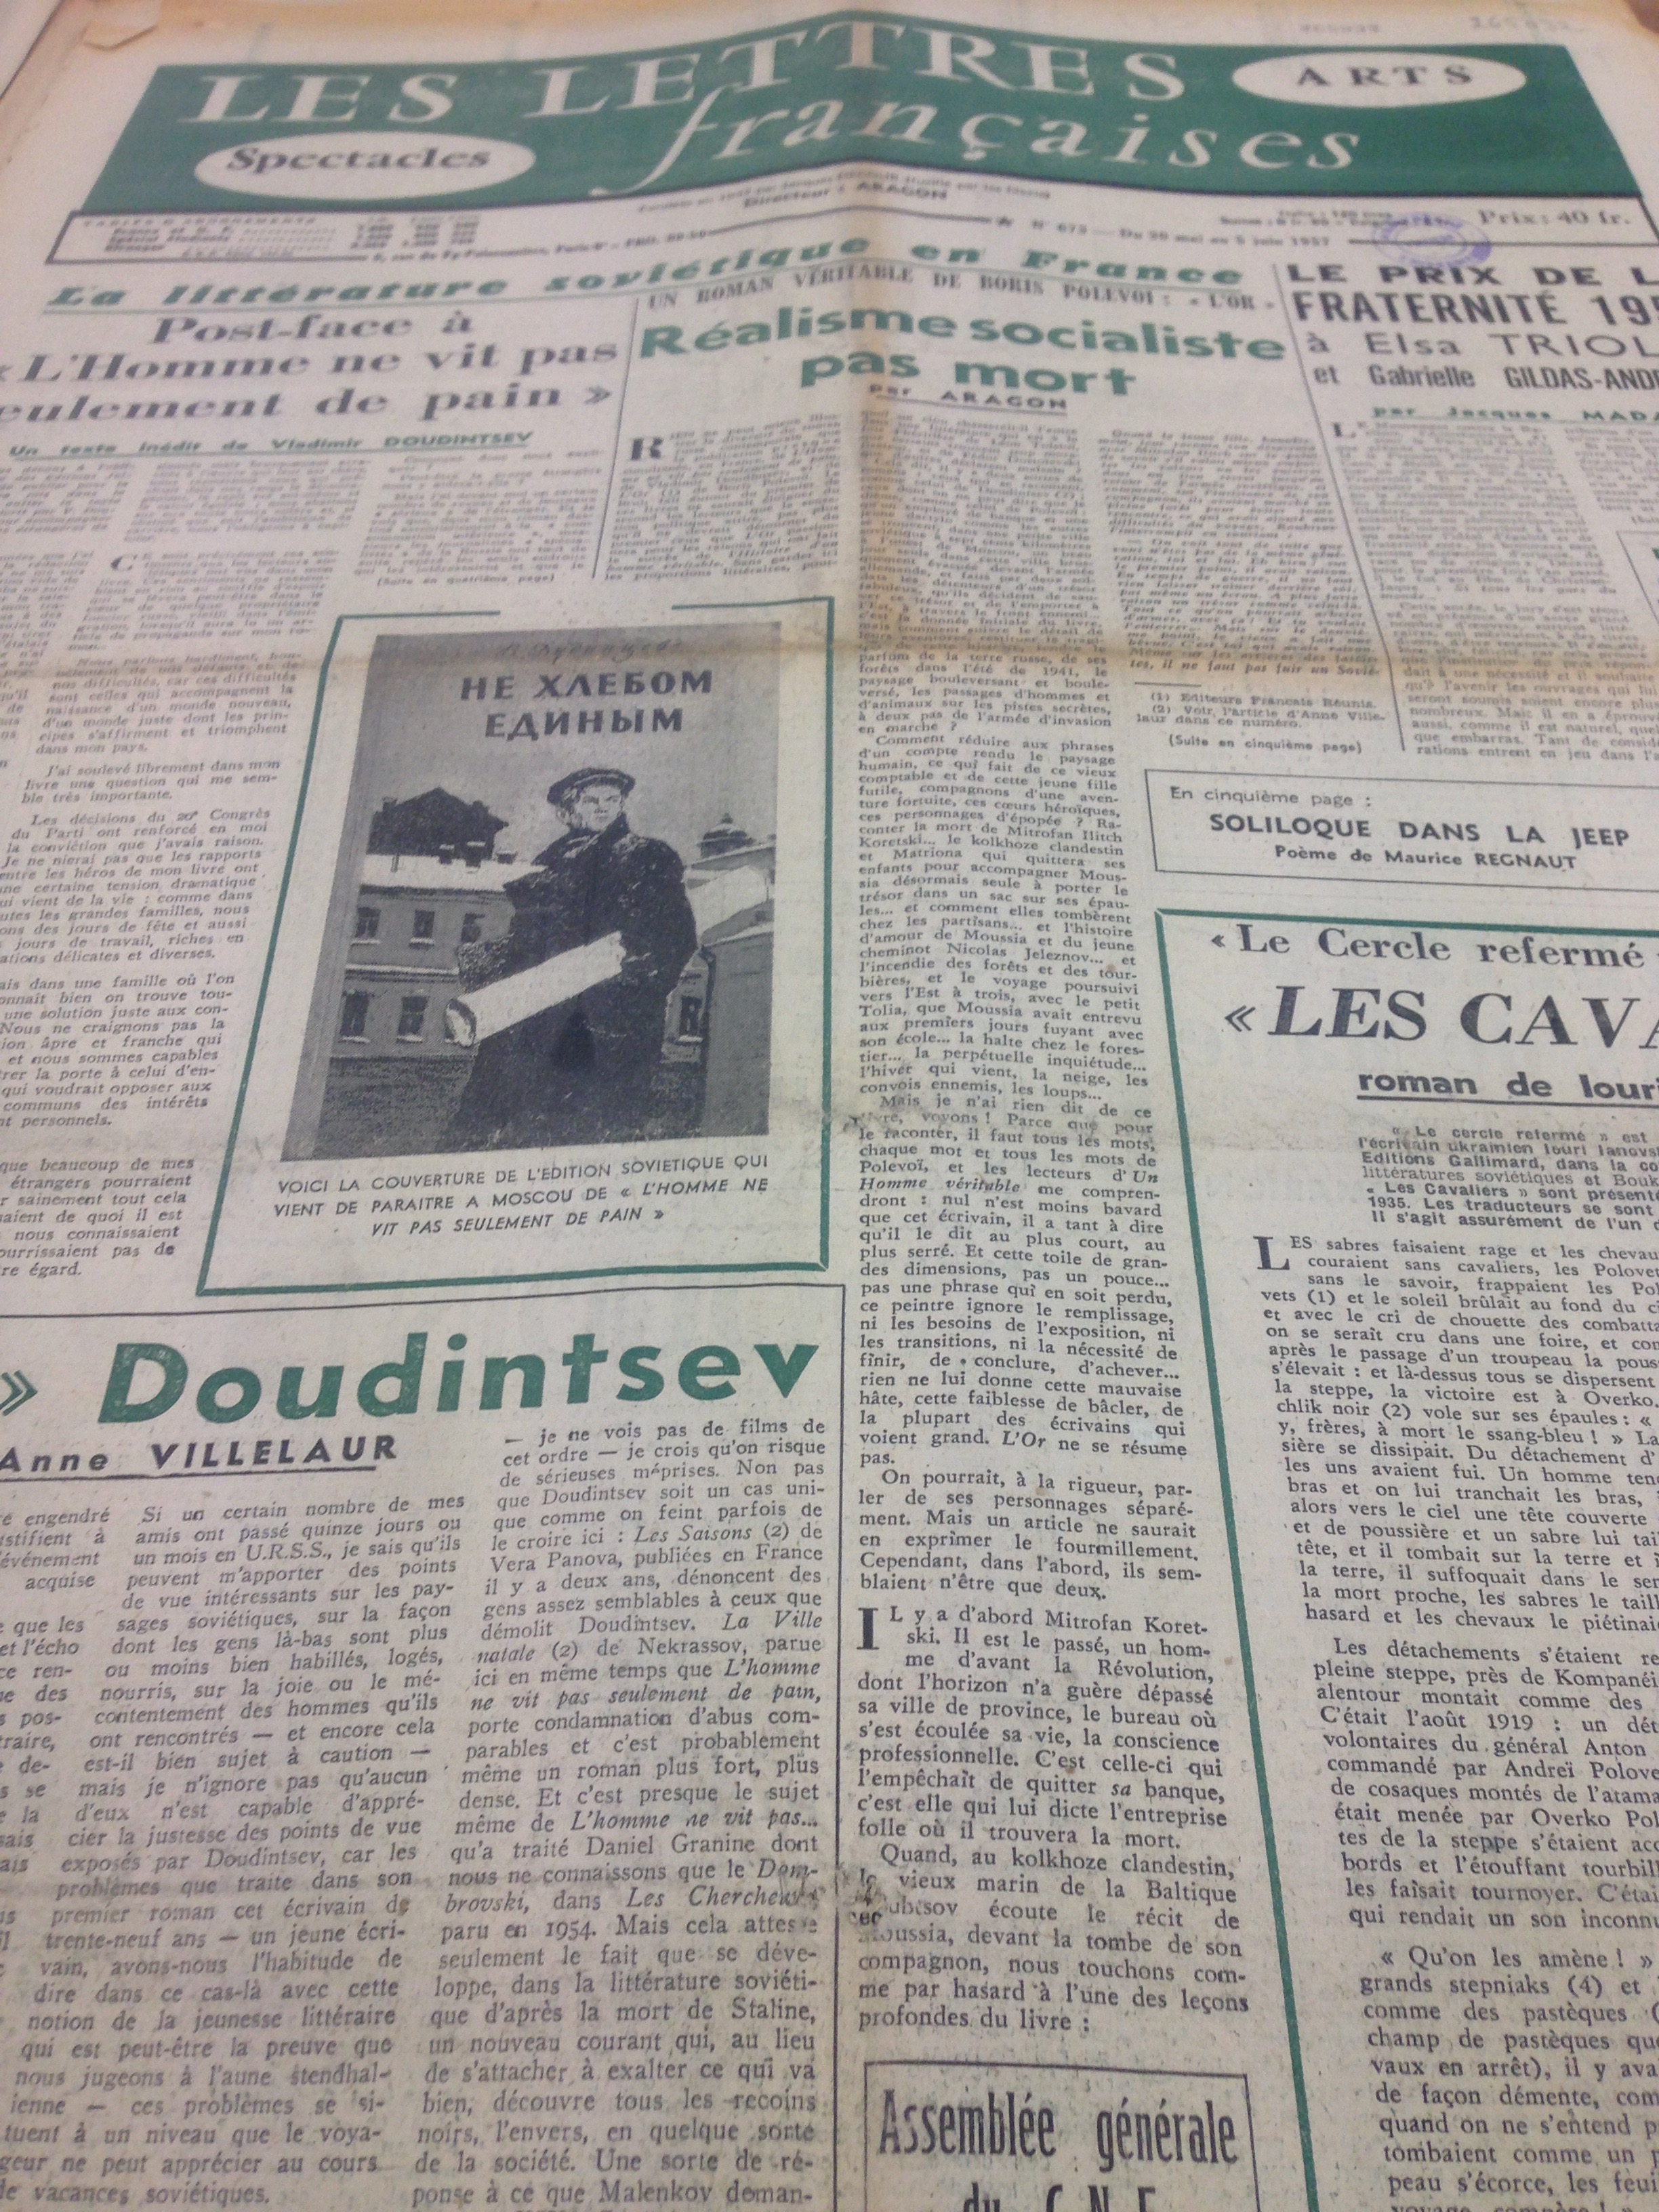
\includegraphics[width=\textwidth,height=\textheight,keepaspectratio]{Annexe/Image1.jpg}
	\caption{\cite{realsoc}}\label{fig:realsoc}
    \end{figure*}

   \begin{figure*}[htp]
   \centering
   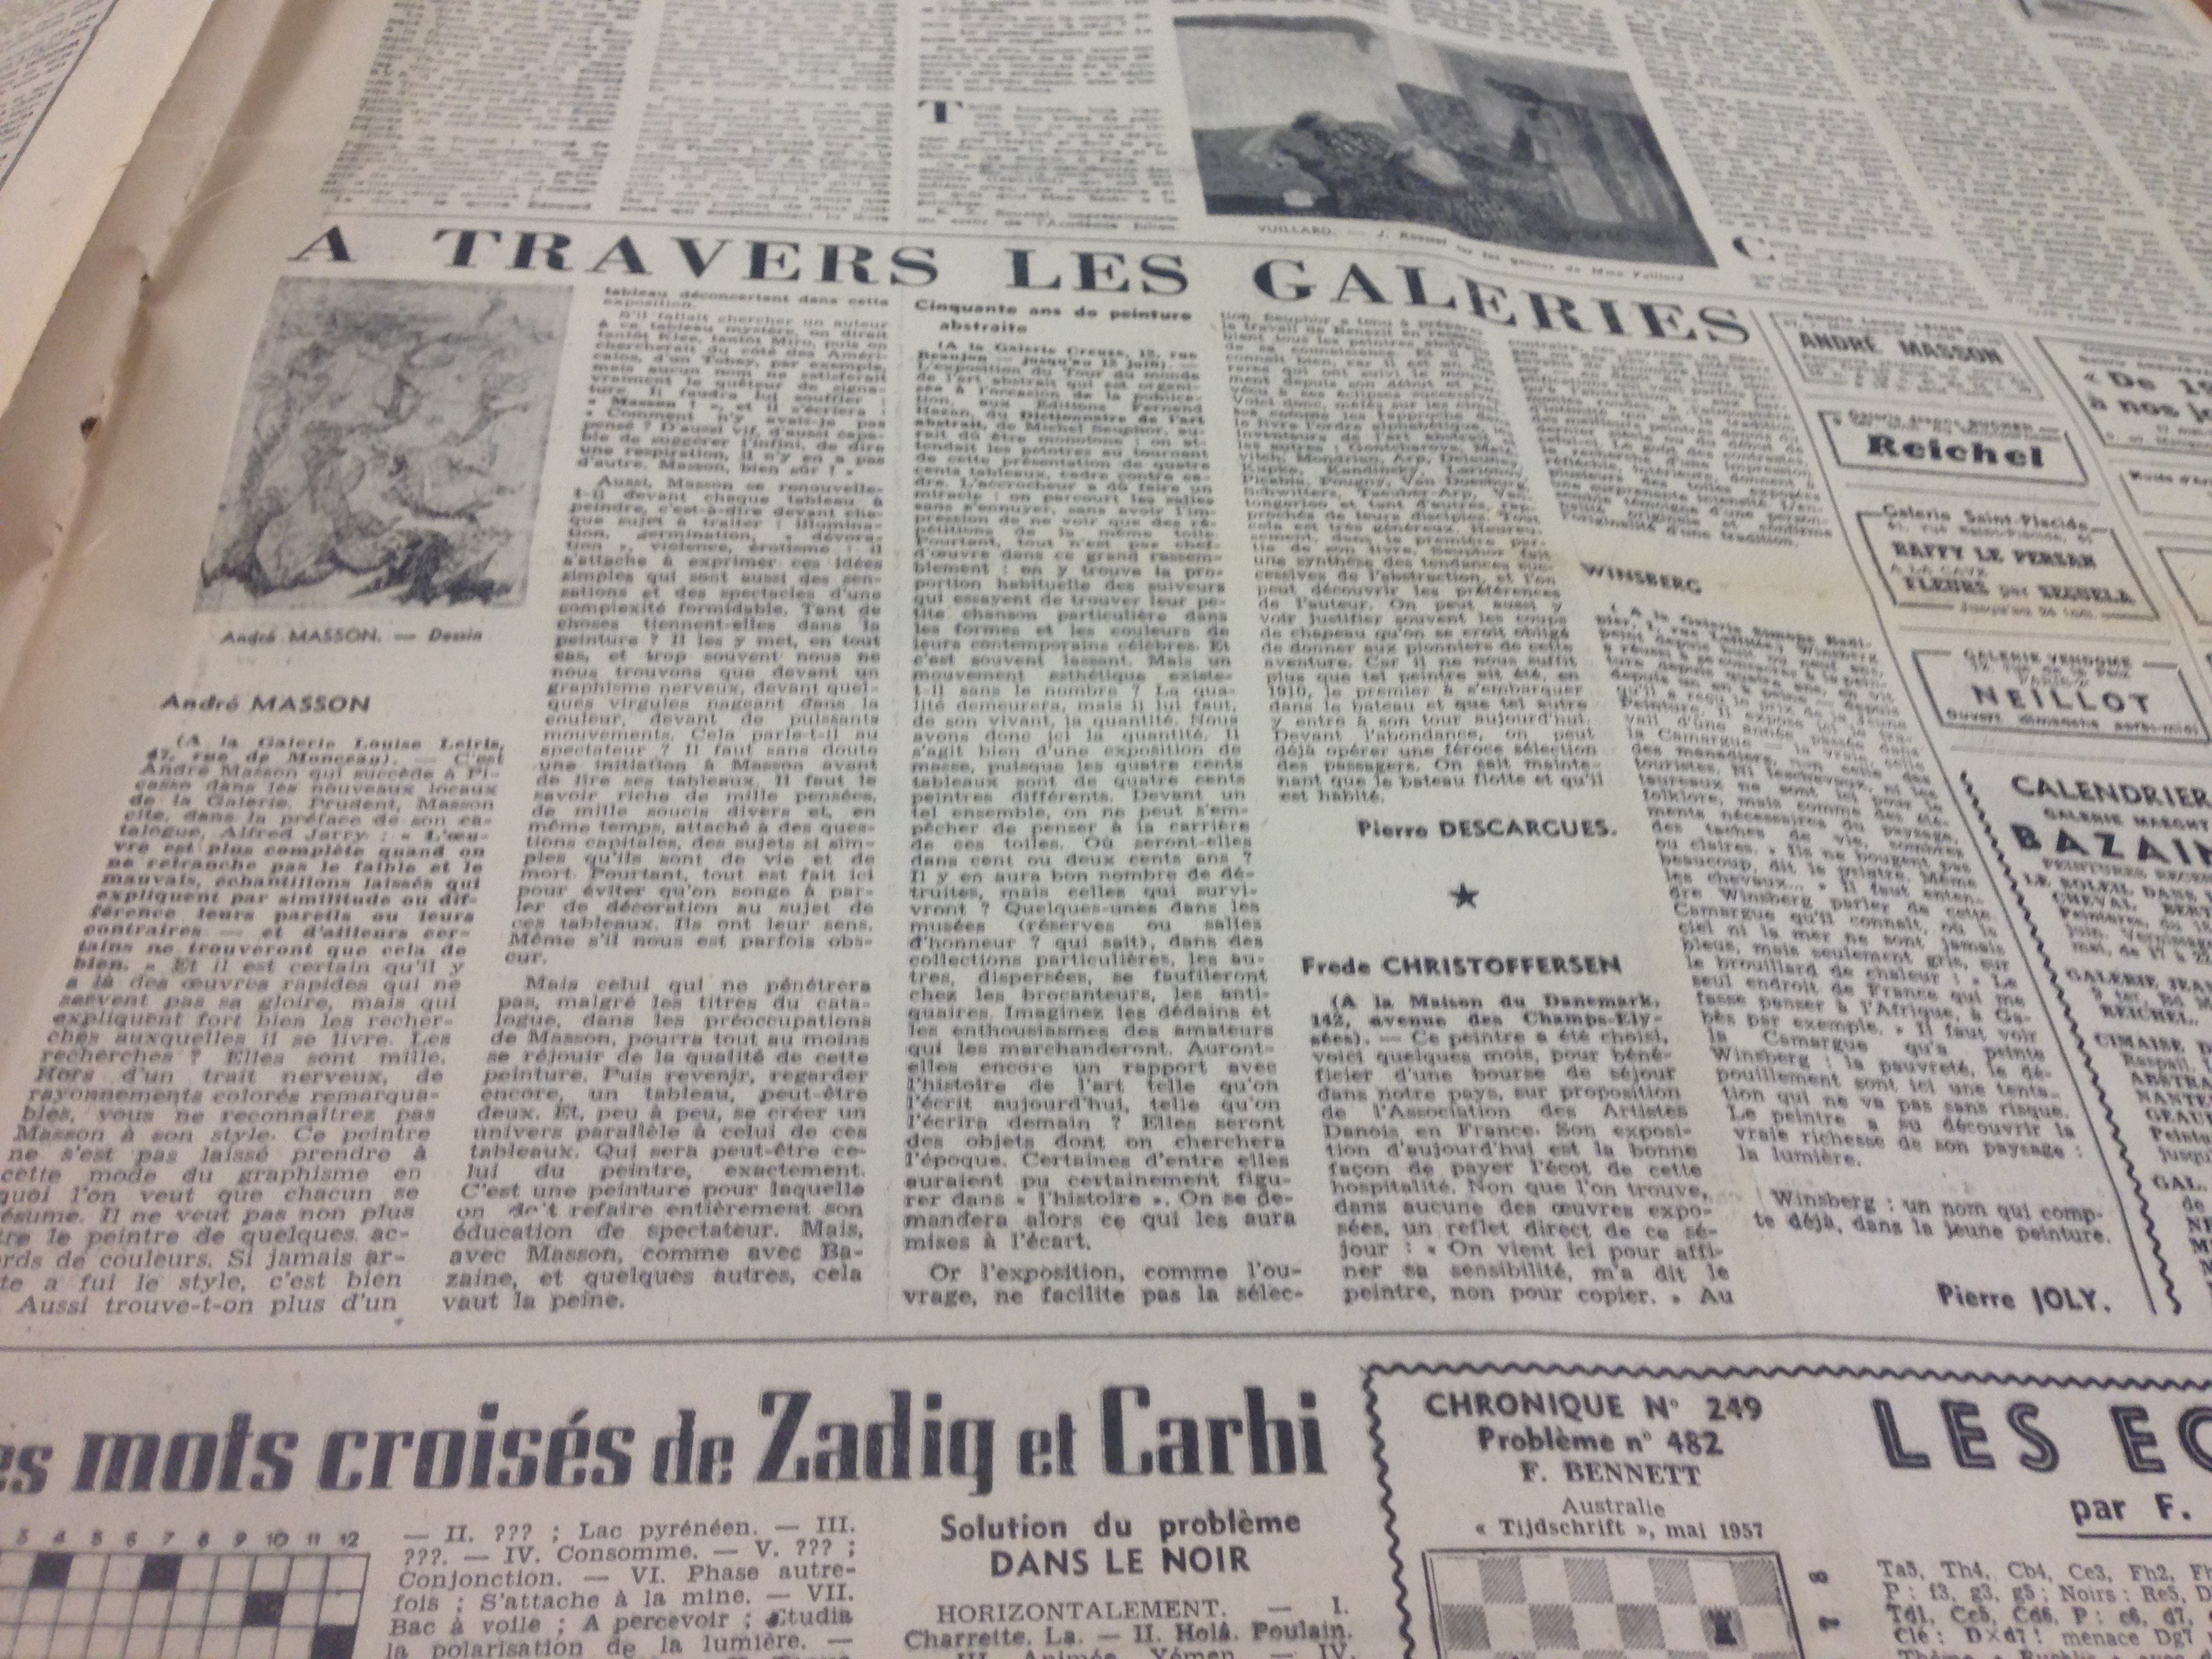
\includegraphics[width=\textwidth,height=\textheight,keepaspectratio]{Annexe/Image8.jpg}
	\caption{\cite{atraversgaleries}}\label{fig:galeries}
    \end{figure*}

  
    \begin{figure*}[htp]
   \centering
   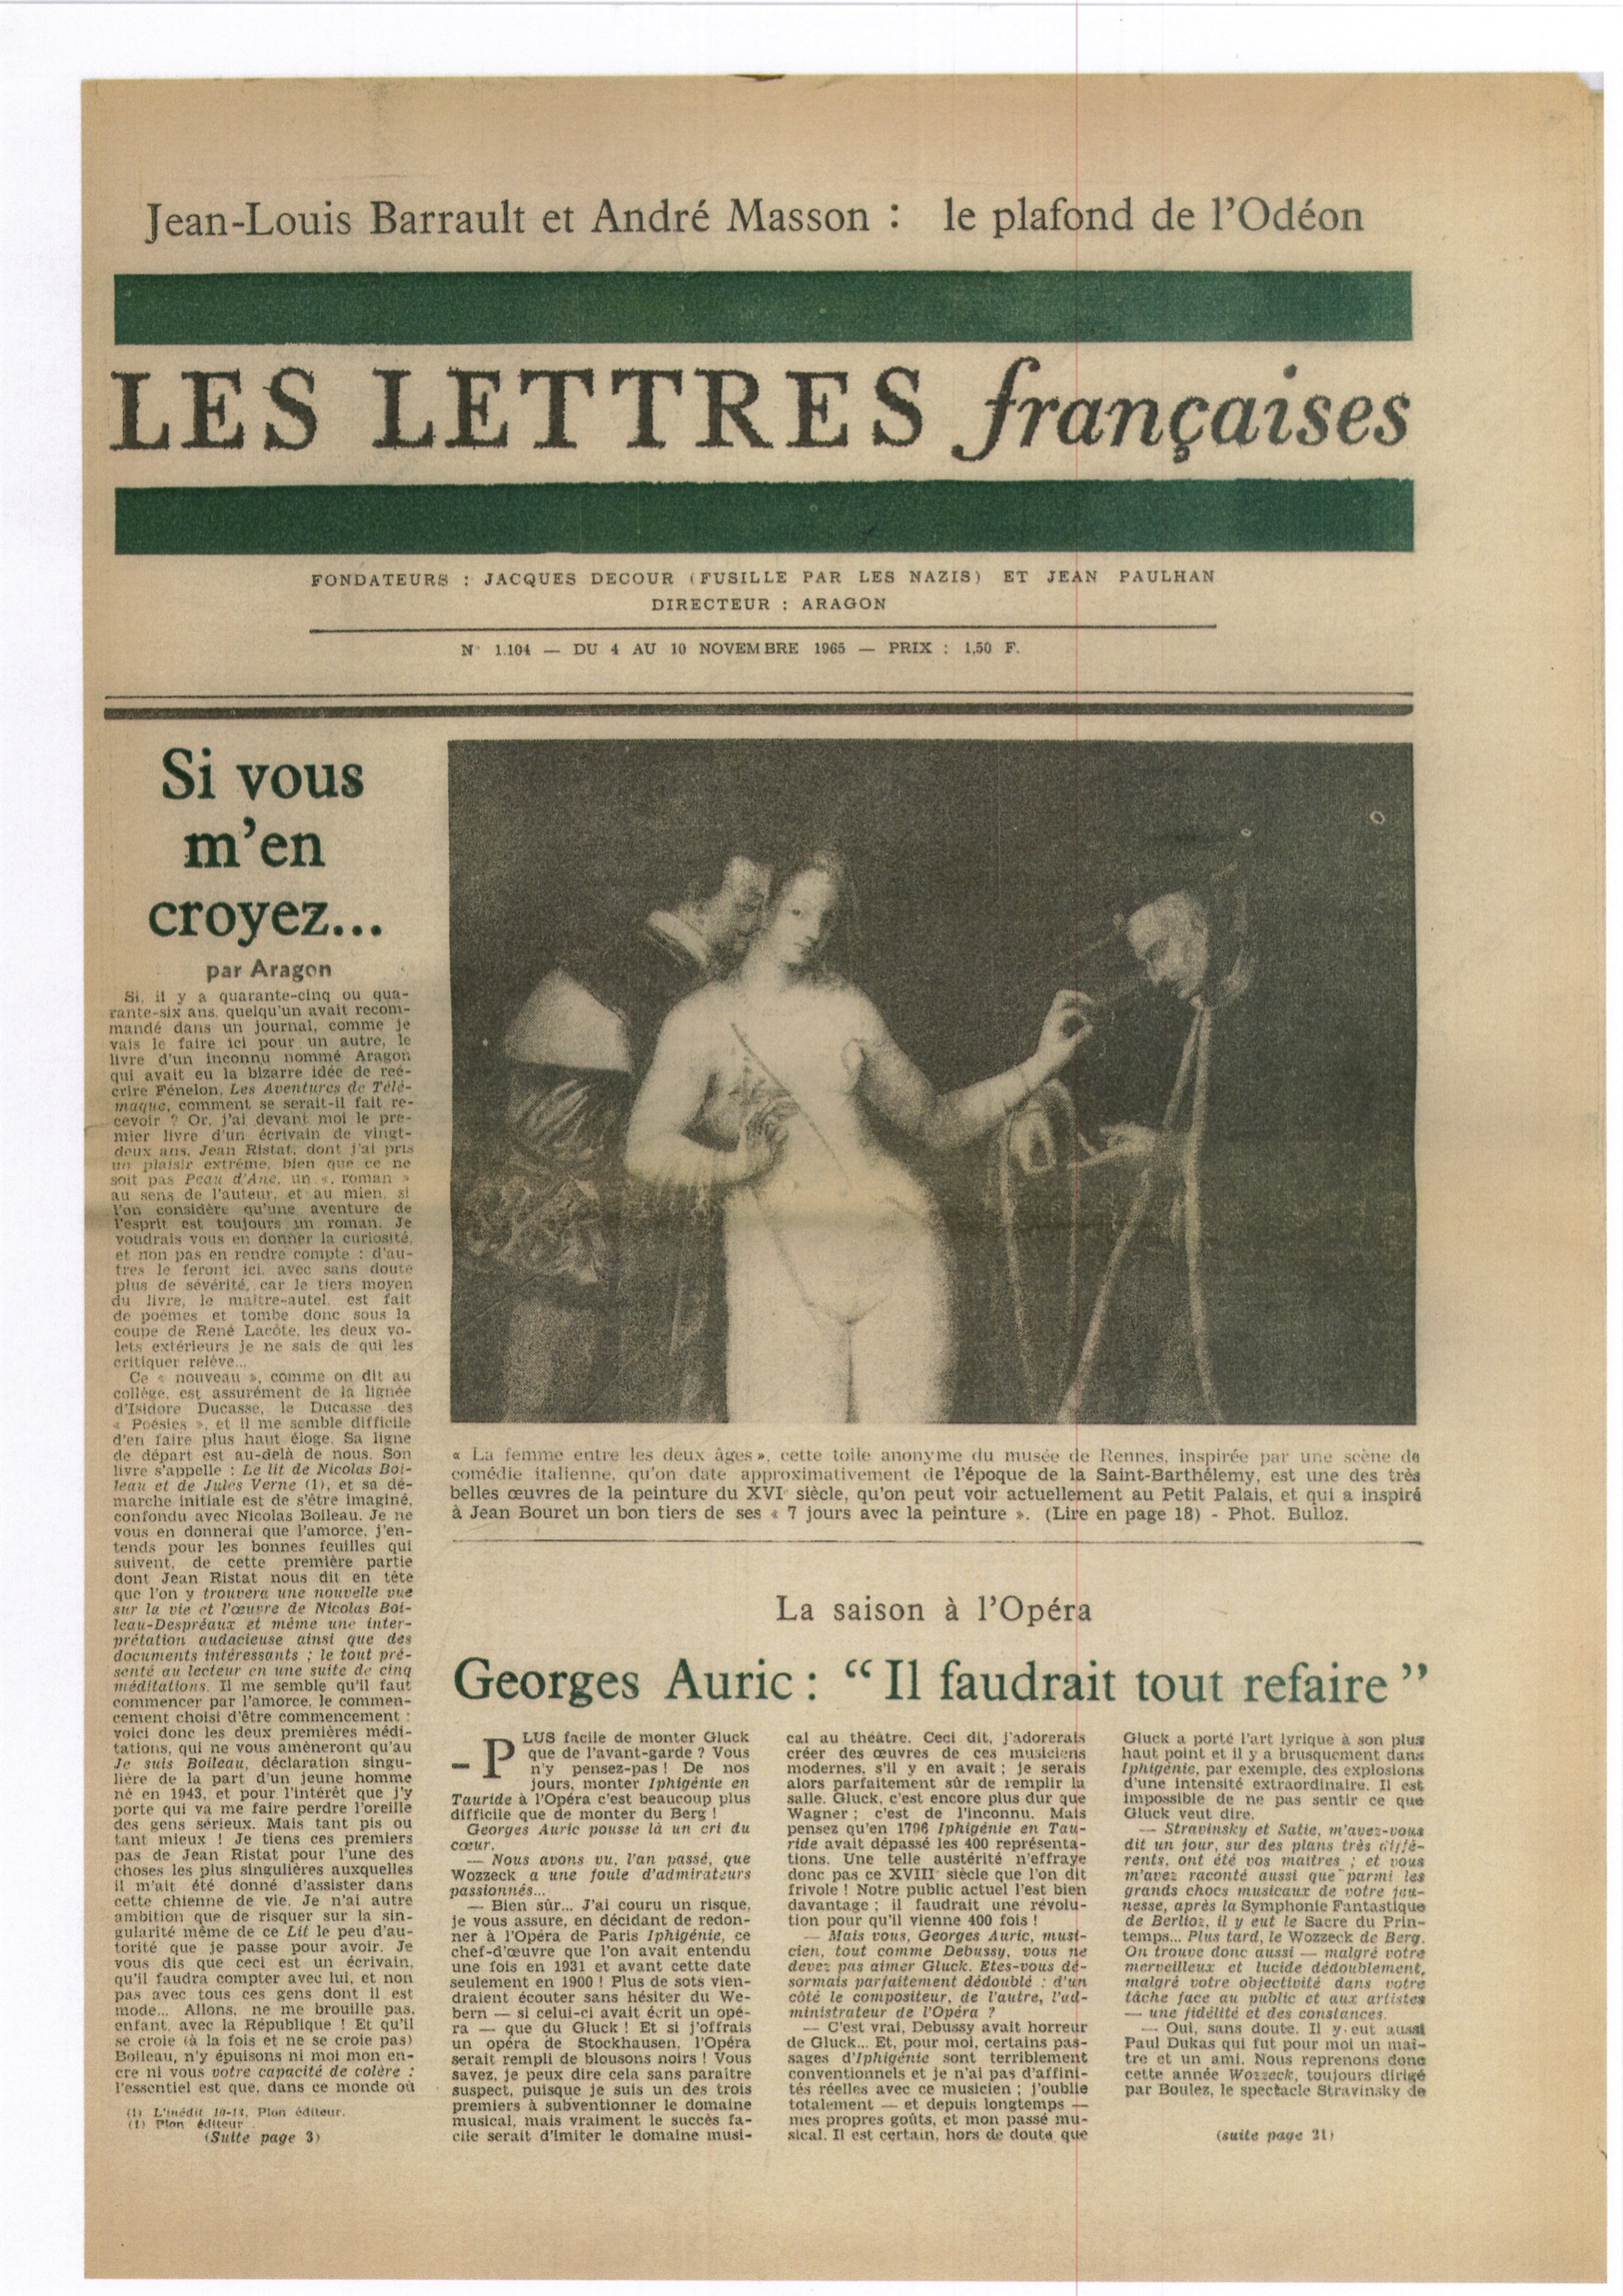
\includegraphics[width=\textwidth,height=\textheight,keepaspectratio]{Annexe/Image36.jpg}
	\caption{\cite{sivous}}\label{fig:sivous}
    \end{figure*}

\begin{figure*}[htp]
   \centering
   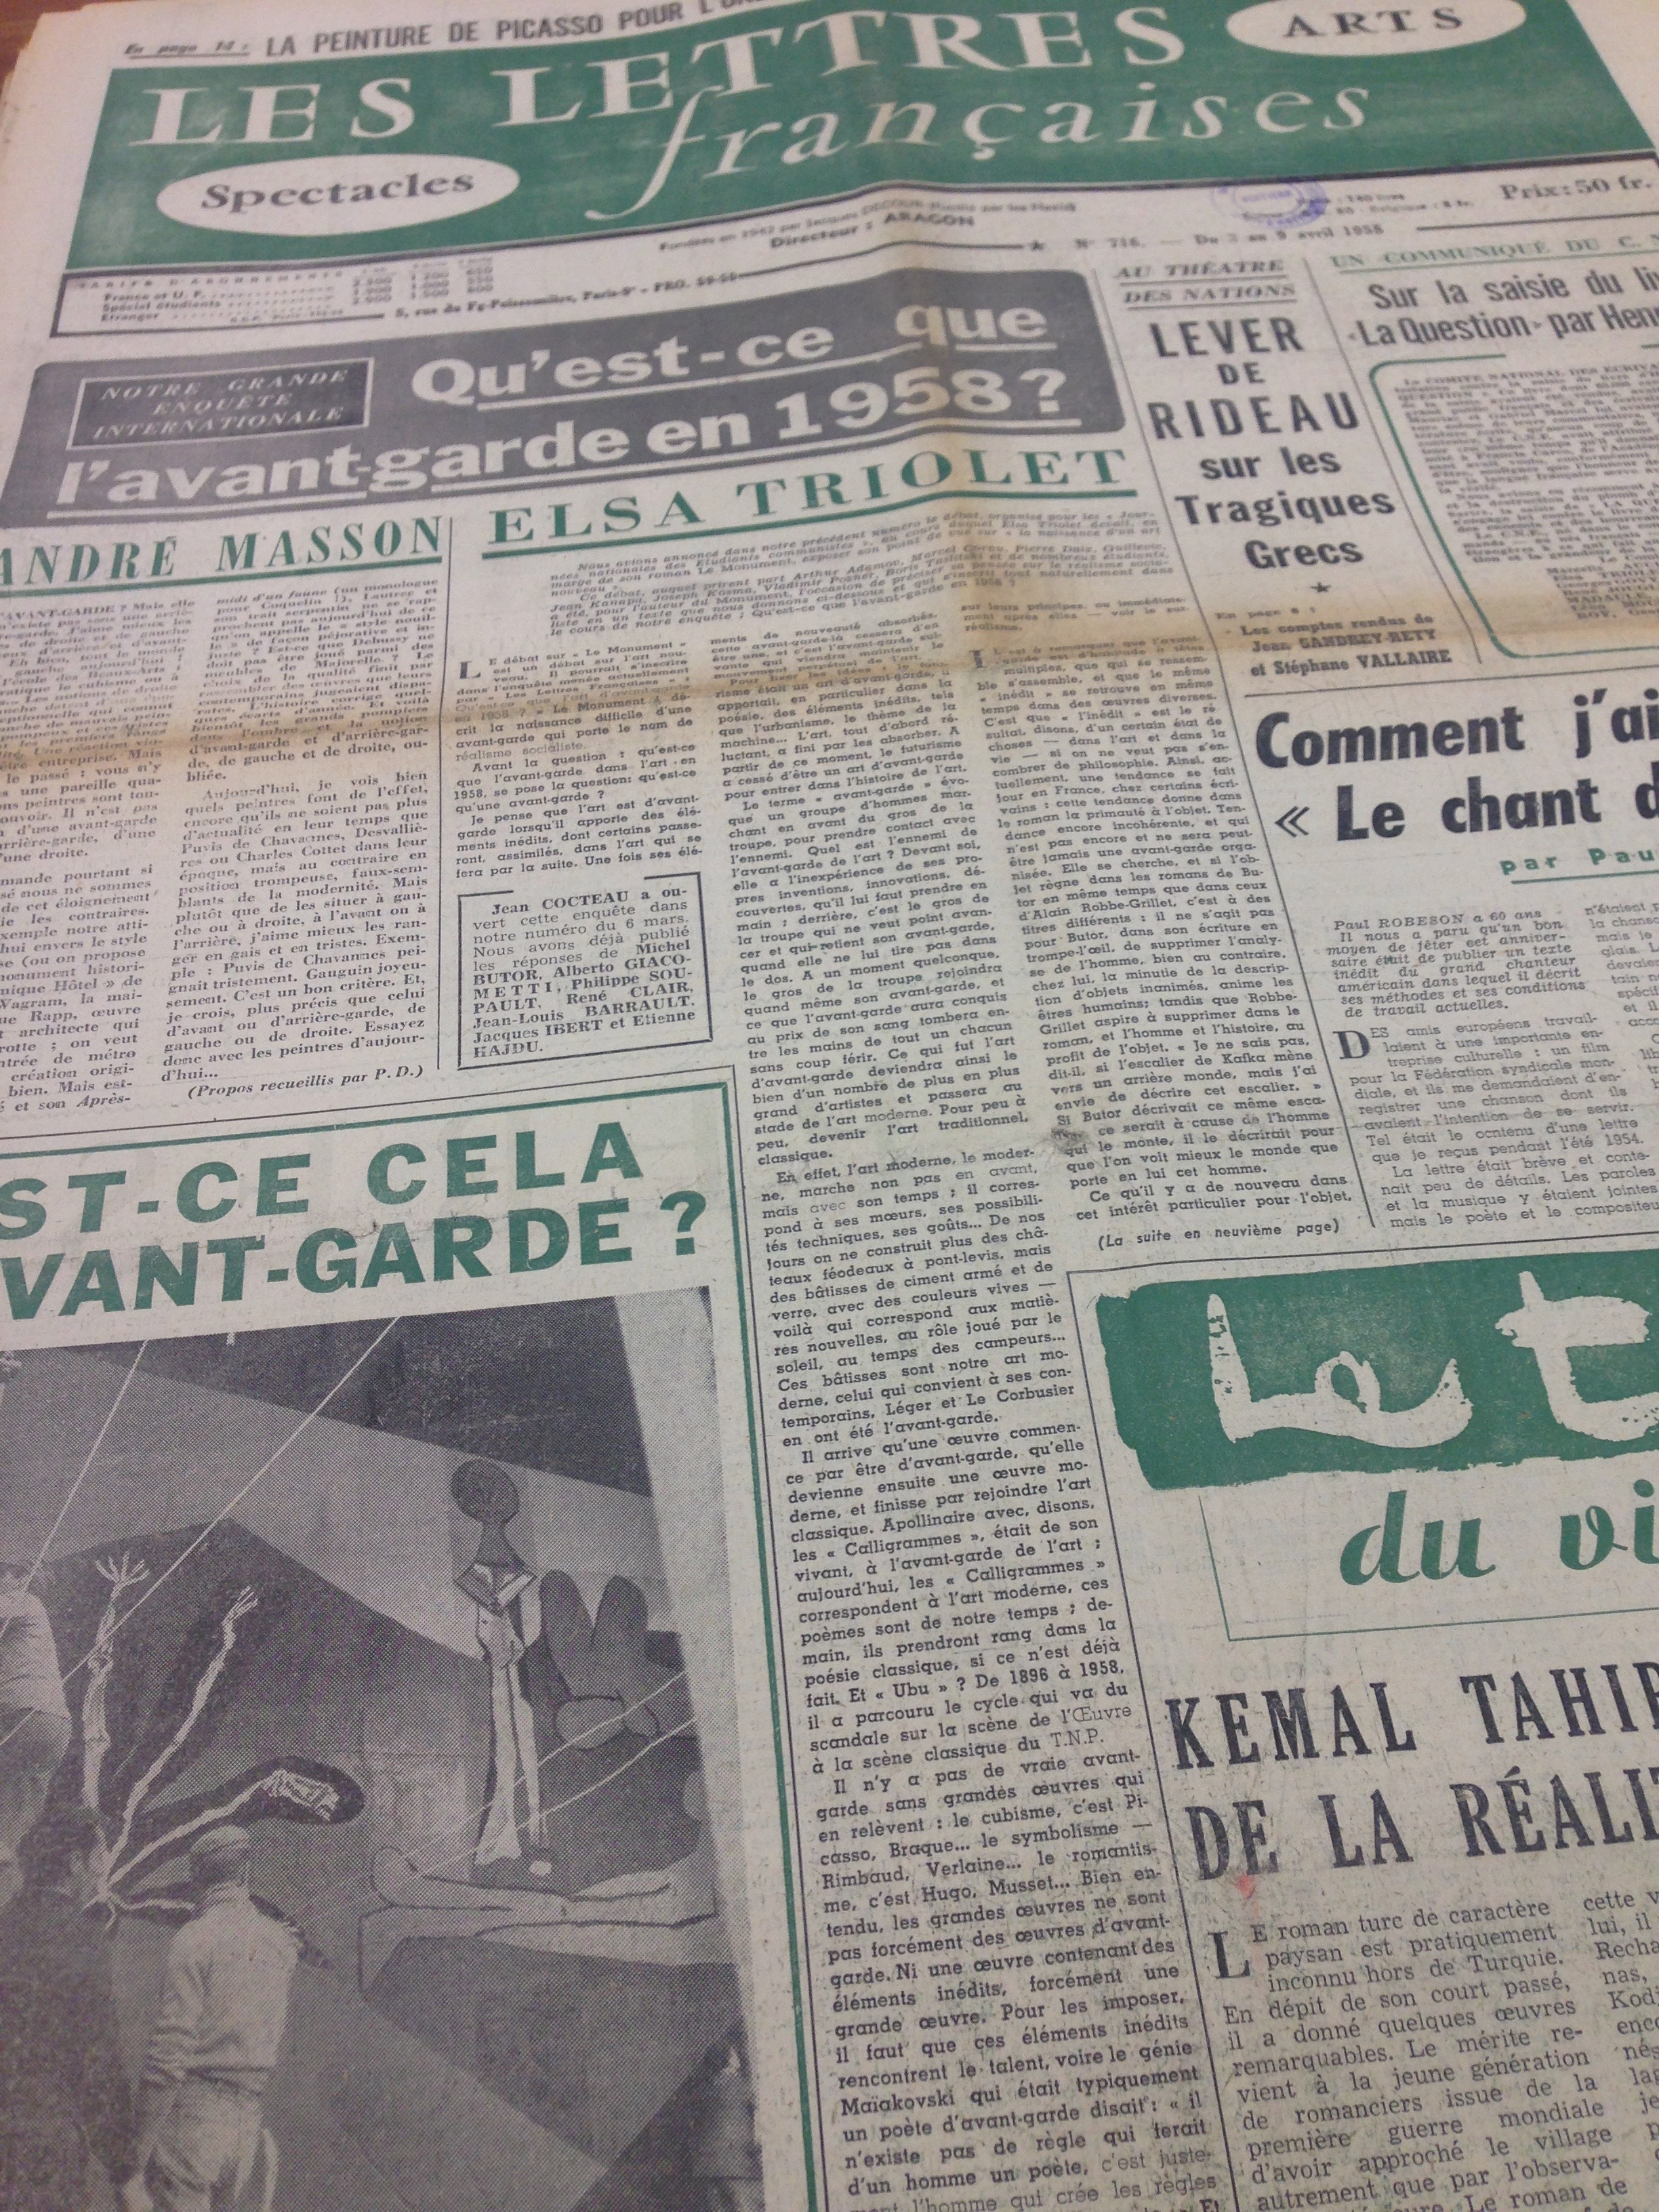
\includegraphics[width=\textwidth,height=\textheight,keepaspectratio]{Annexe/Image34.jpg}
	\caption{\cite{avantgarde}}\label{fig:avantgarde1}
    \end{figure*}


    \begin{figure*}[htp]
   \centering
   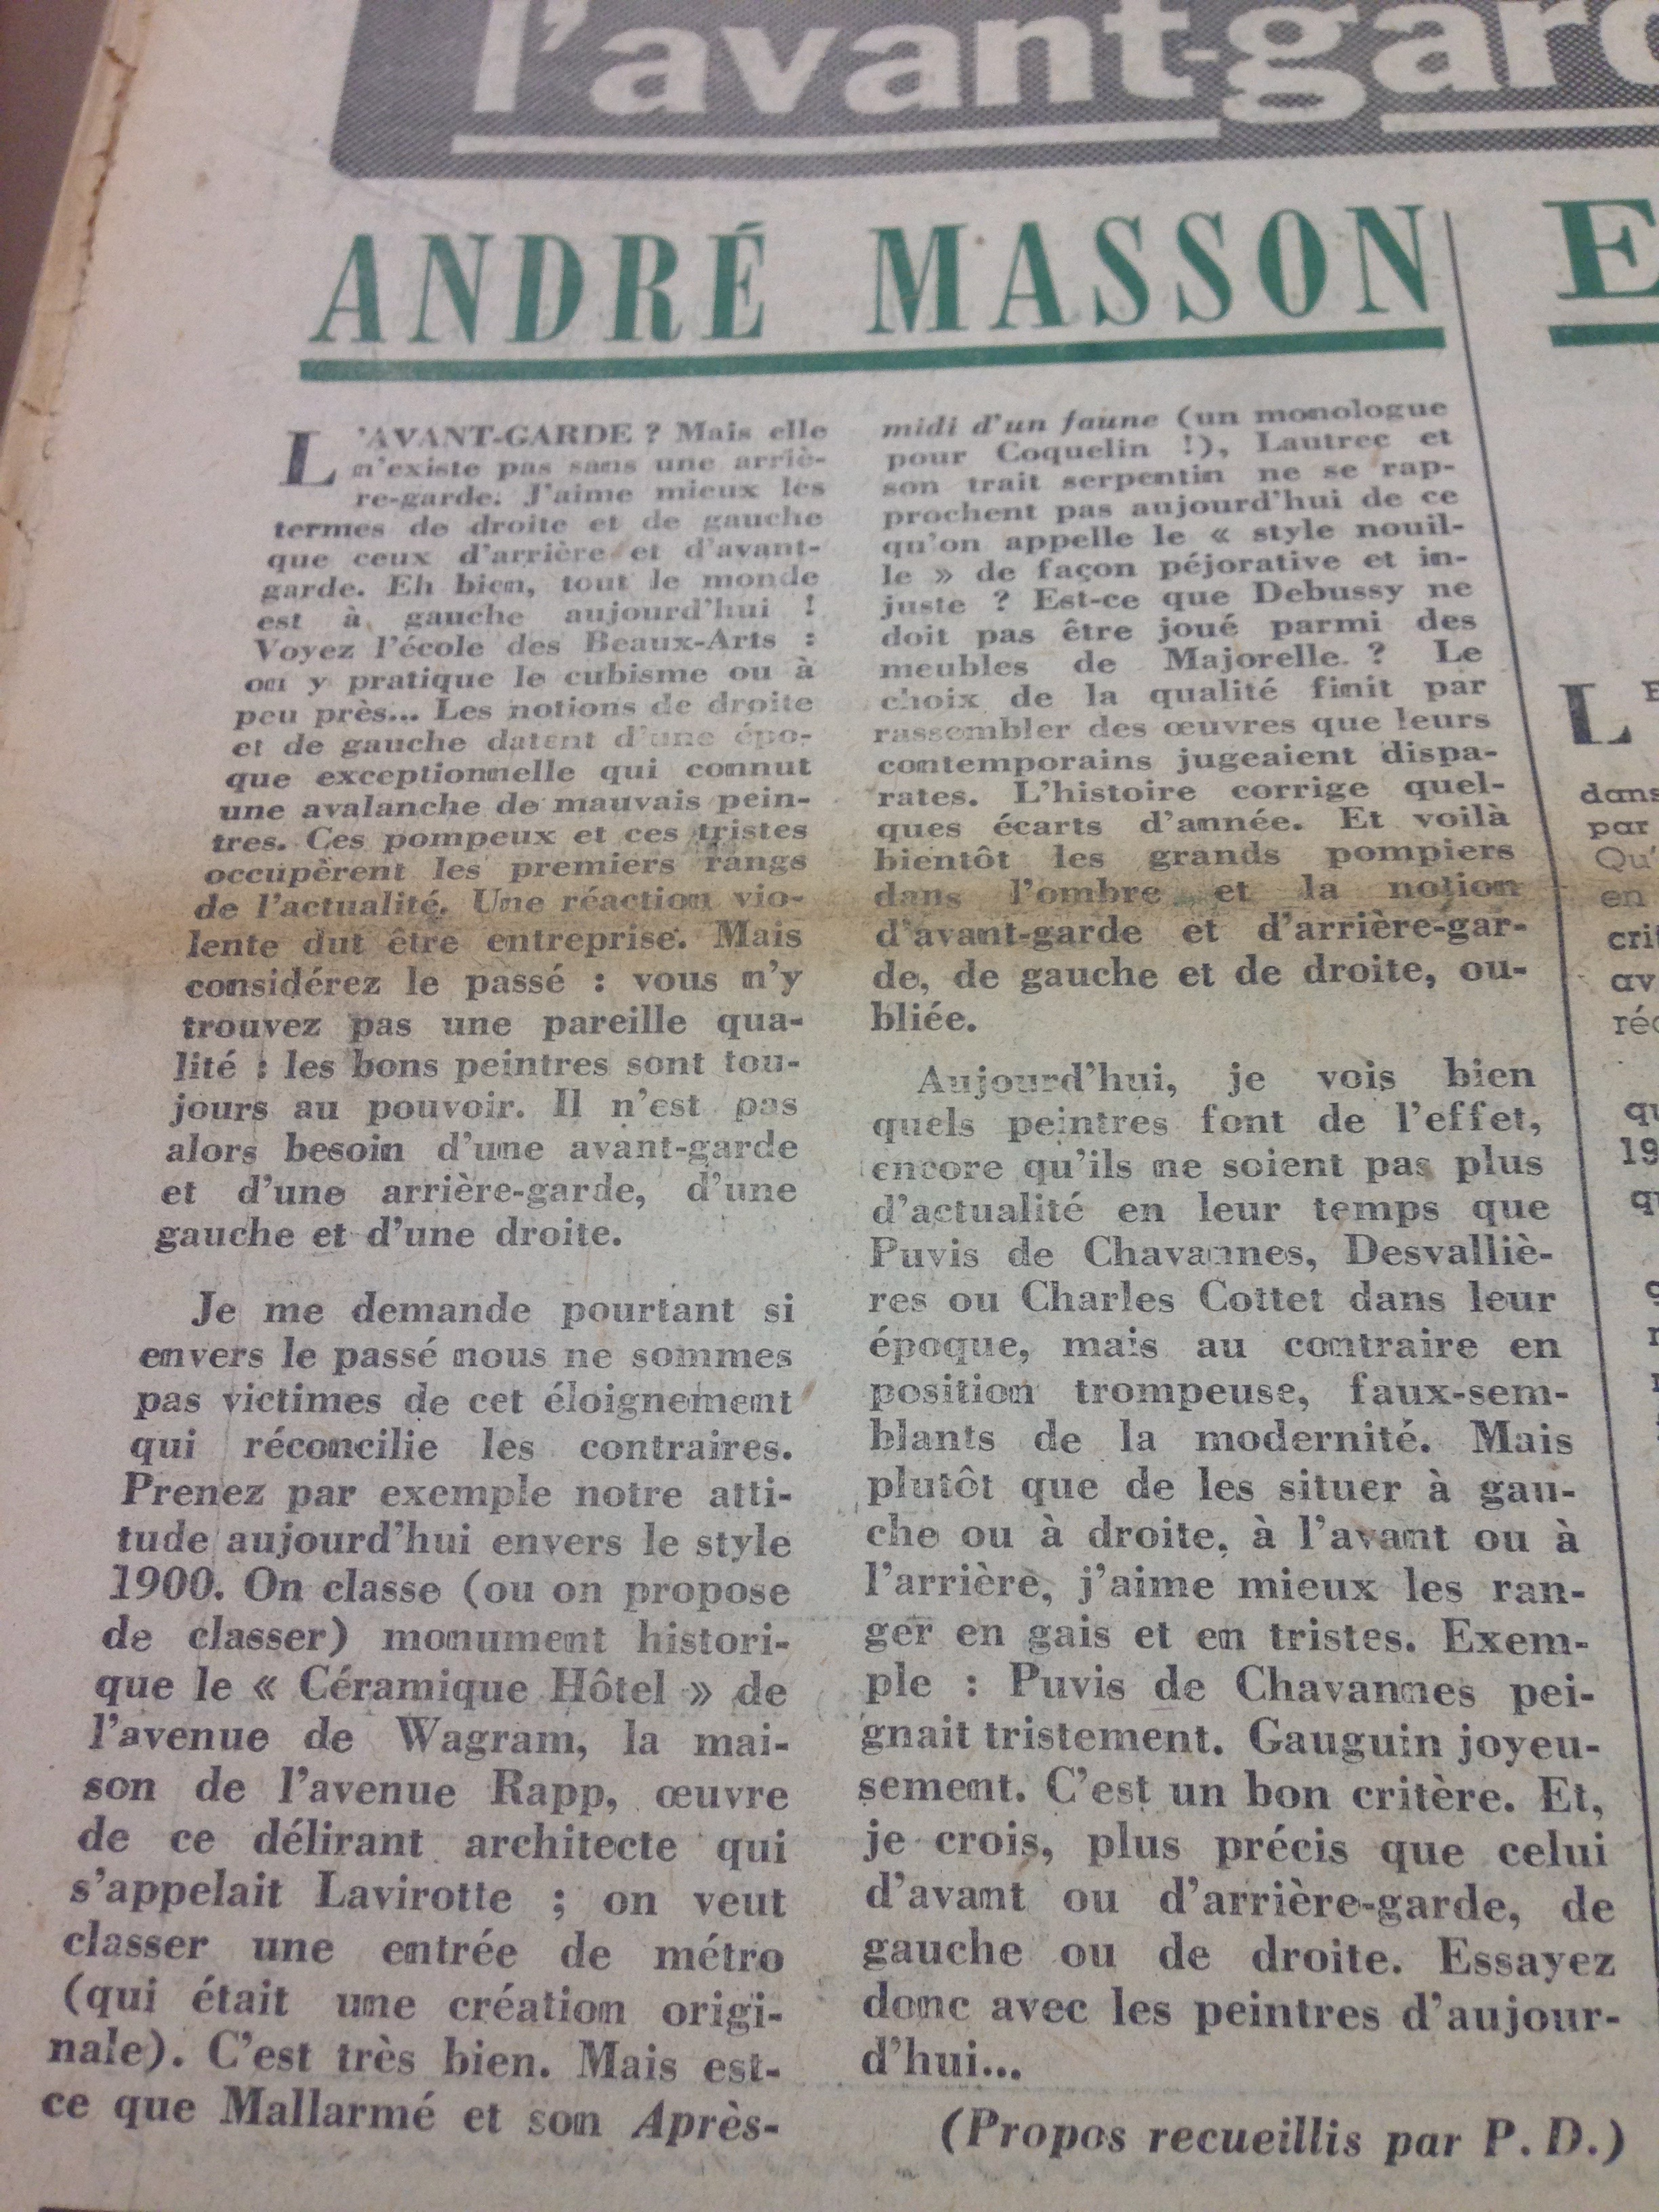
\includegraphics[width=\textwidth,height=\textheight,keepaspectratio]{Annexe/Image21.jpg}
	\caption{\cite{avantgarde}}\label{fig:avantgardemasson}
    \end{figure*}

    \begin{figure*}[htp]
   \centering
   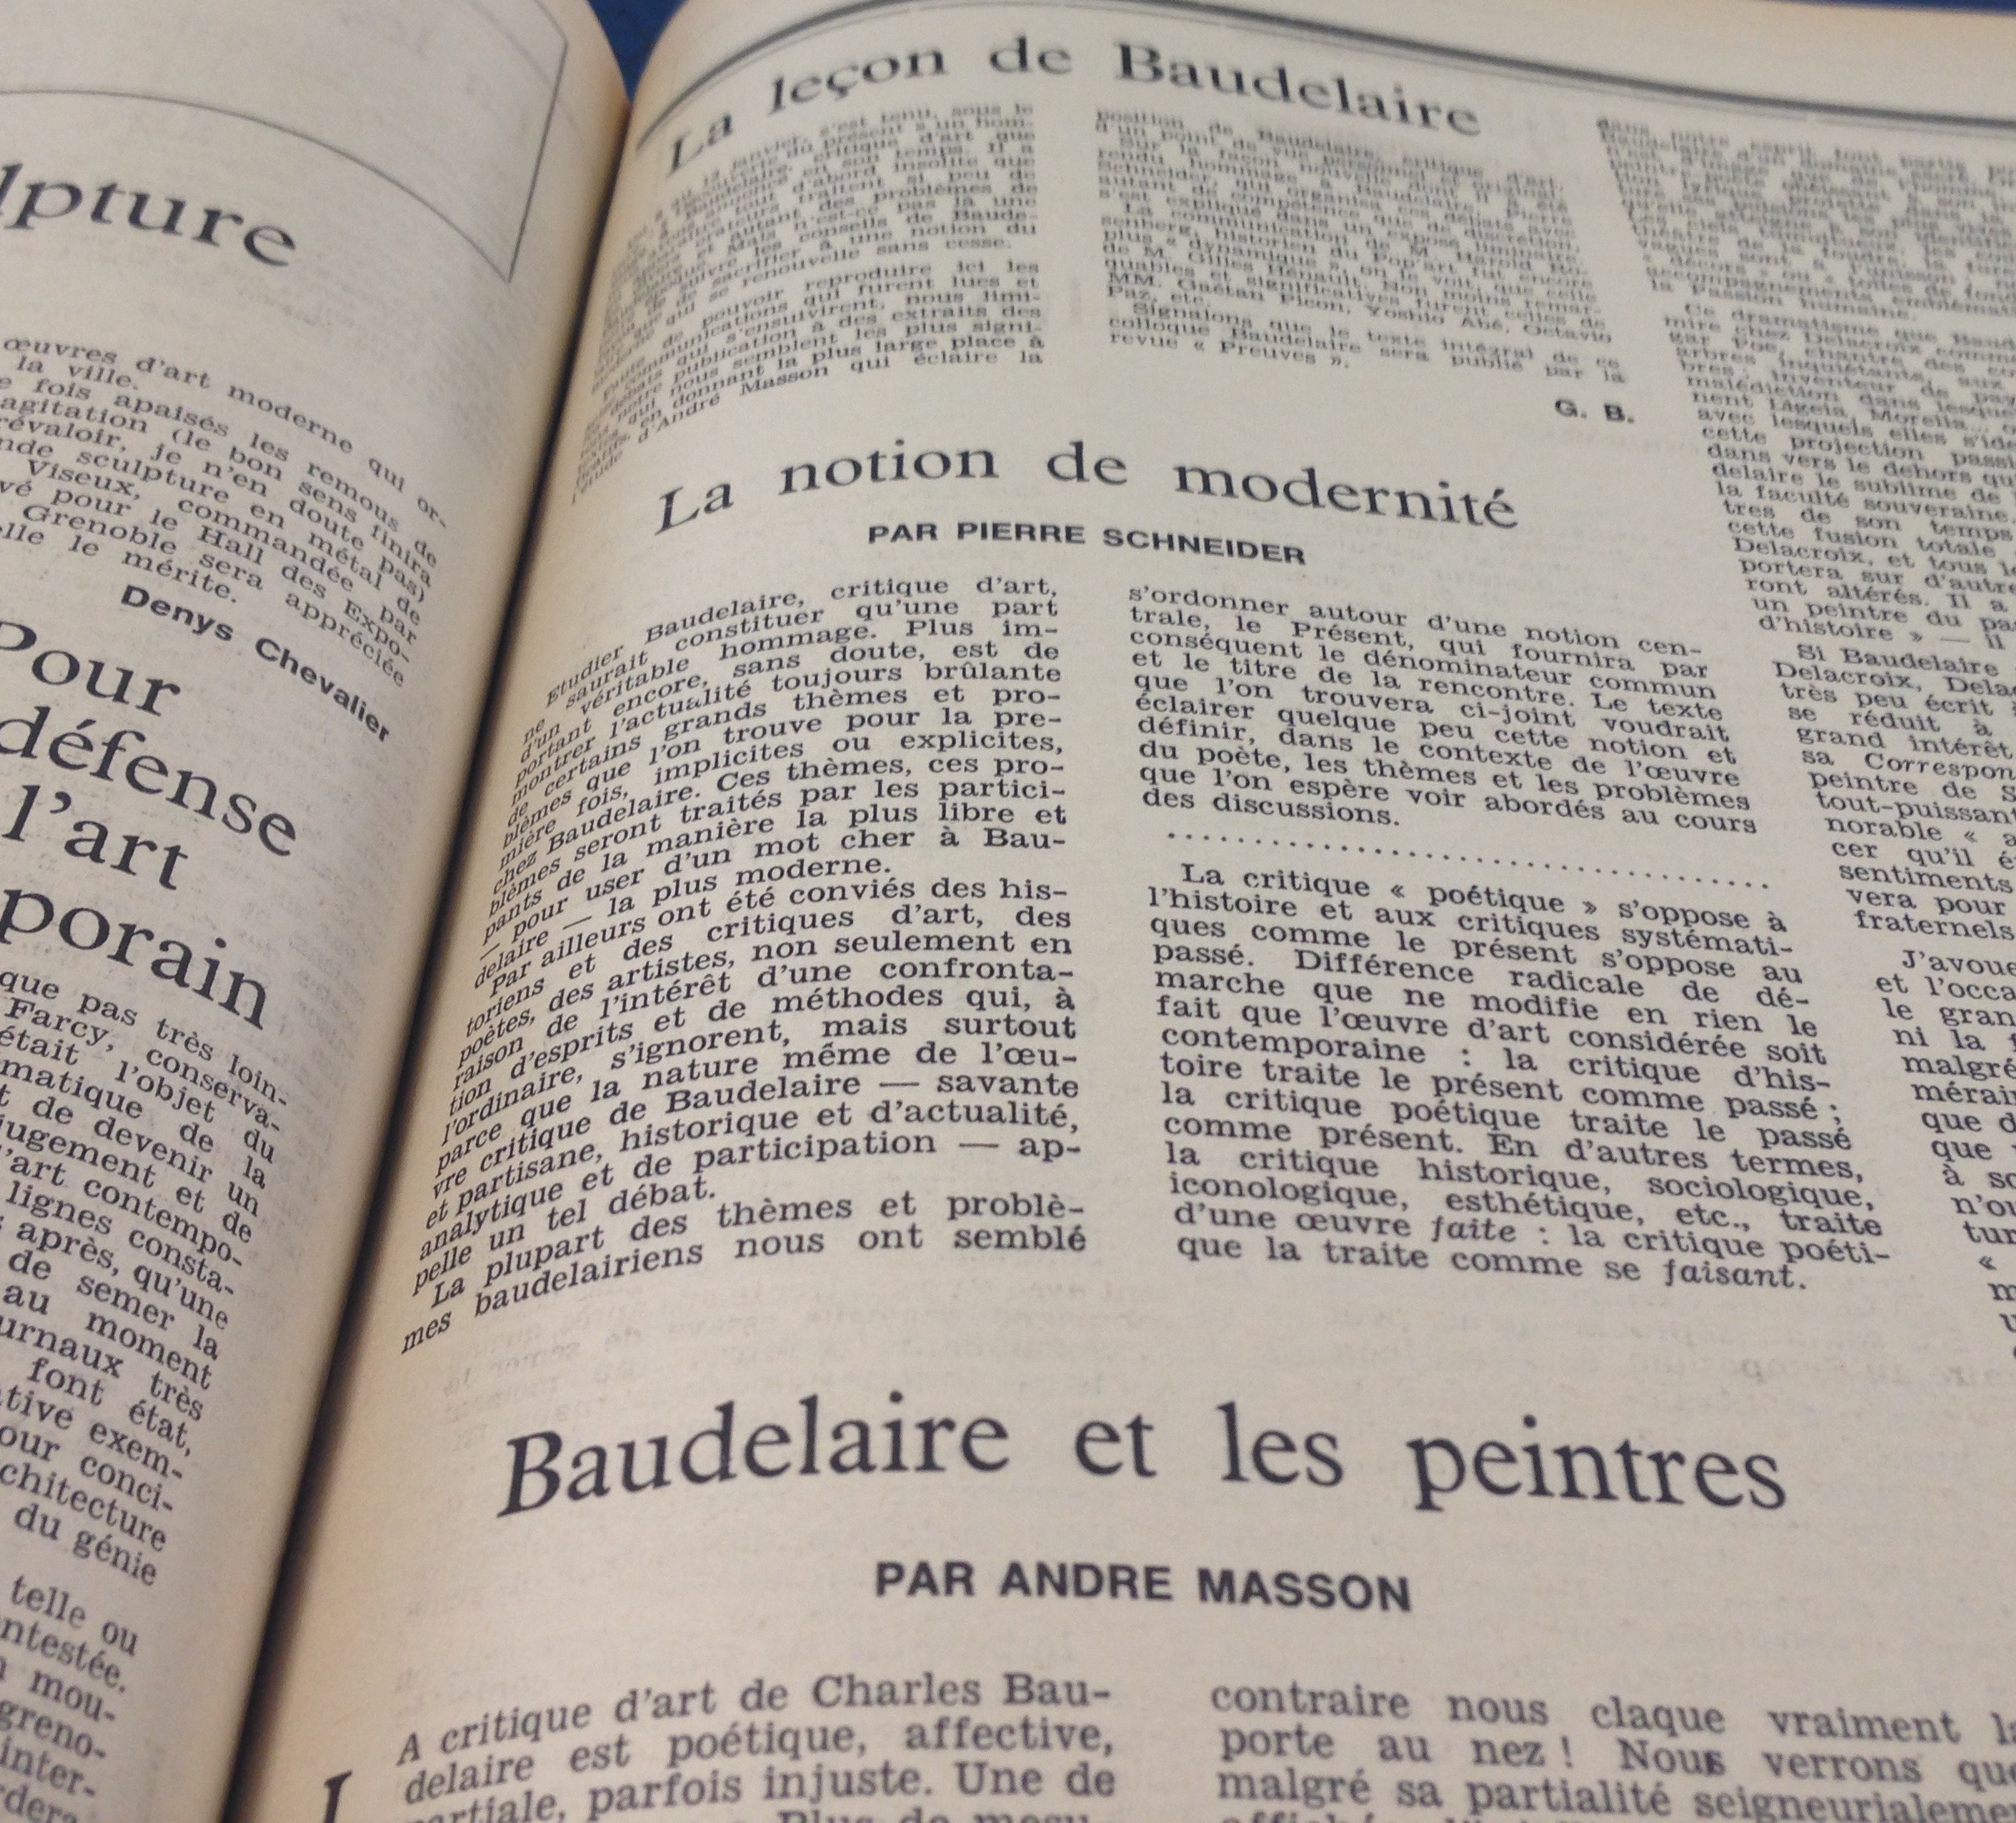
\includegraphics[width=\textwidth,height=\textheight,keepaspectratio]{Annexe/Image3.jpg}
	\caption{\cite{baudelairepeintres}}\label{fig:baudelaire}
    \end{figure*}

    \begin{figure*}[htp]
   \centering
   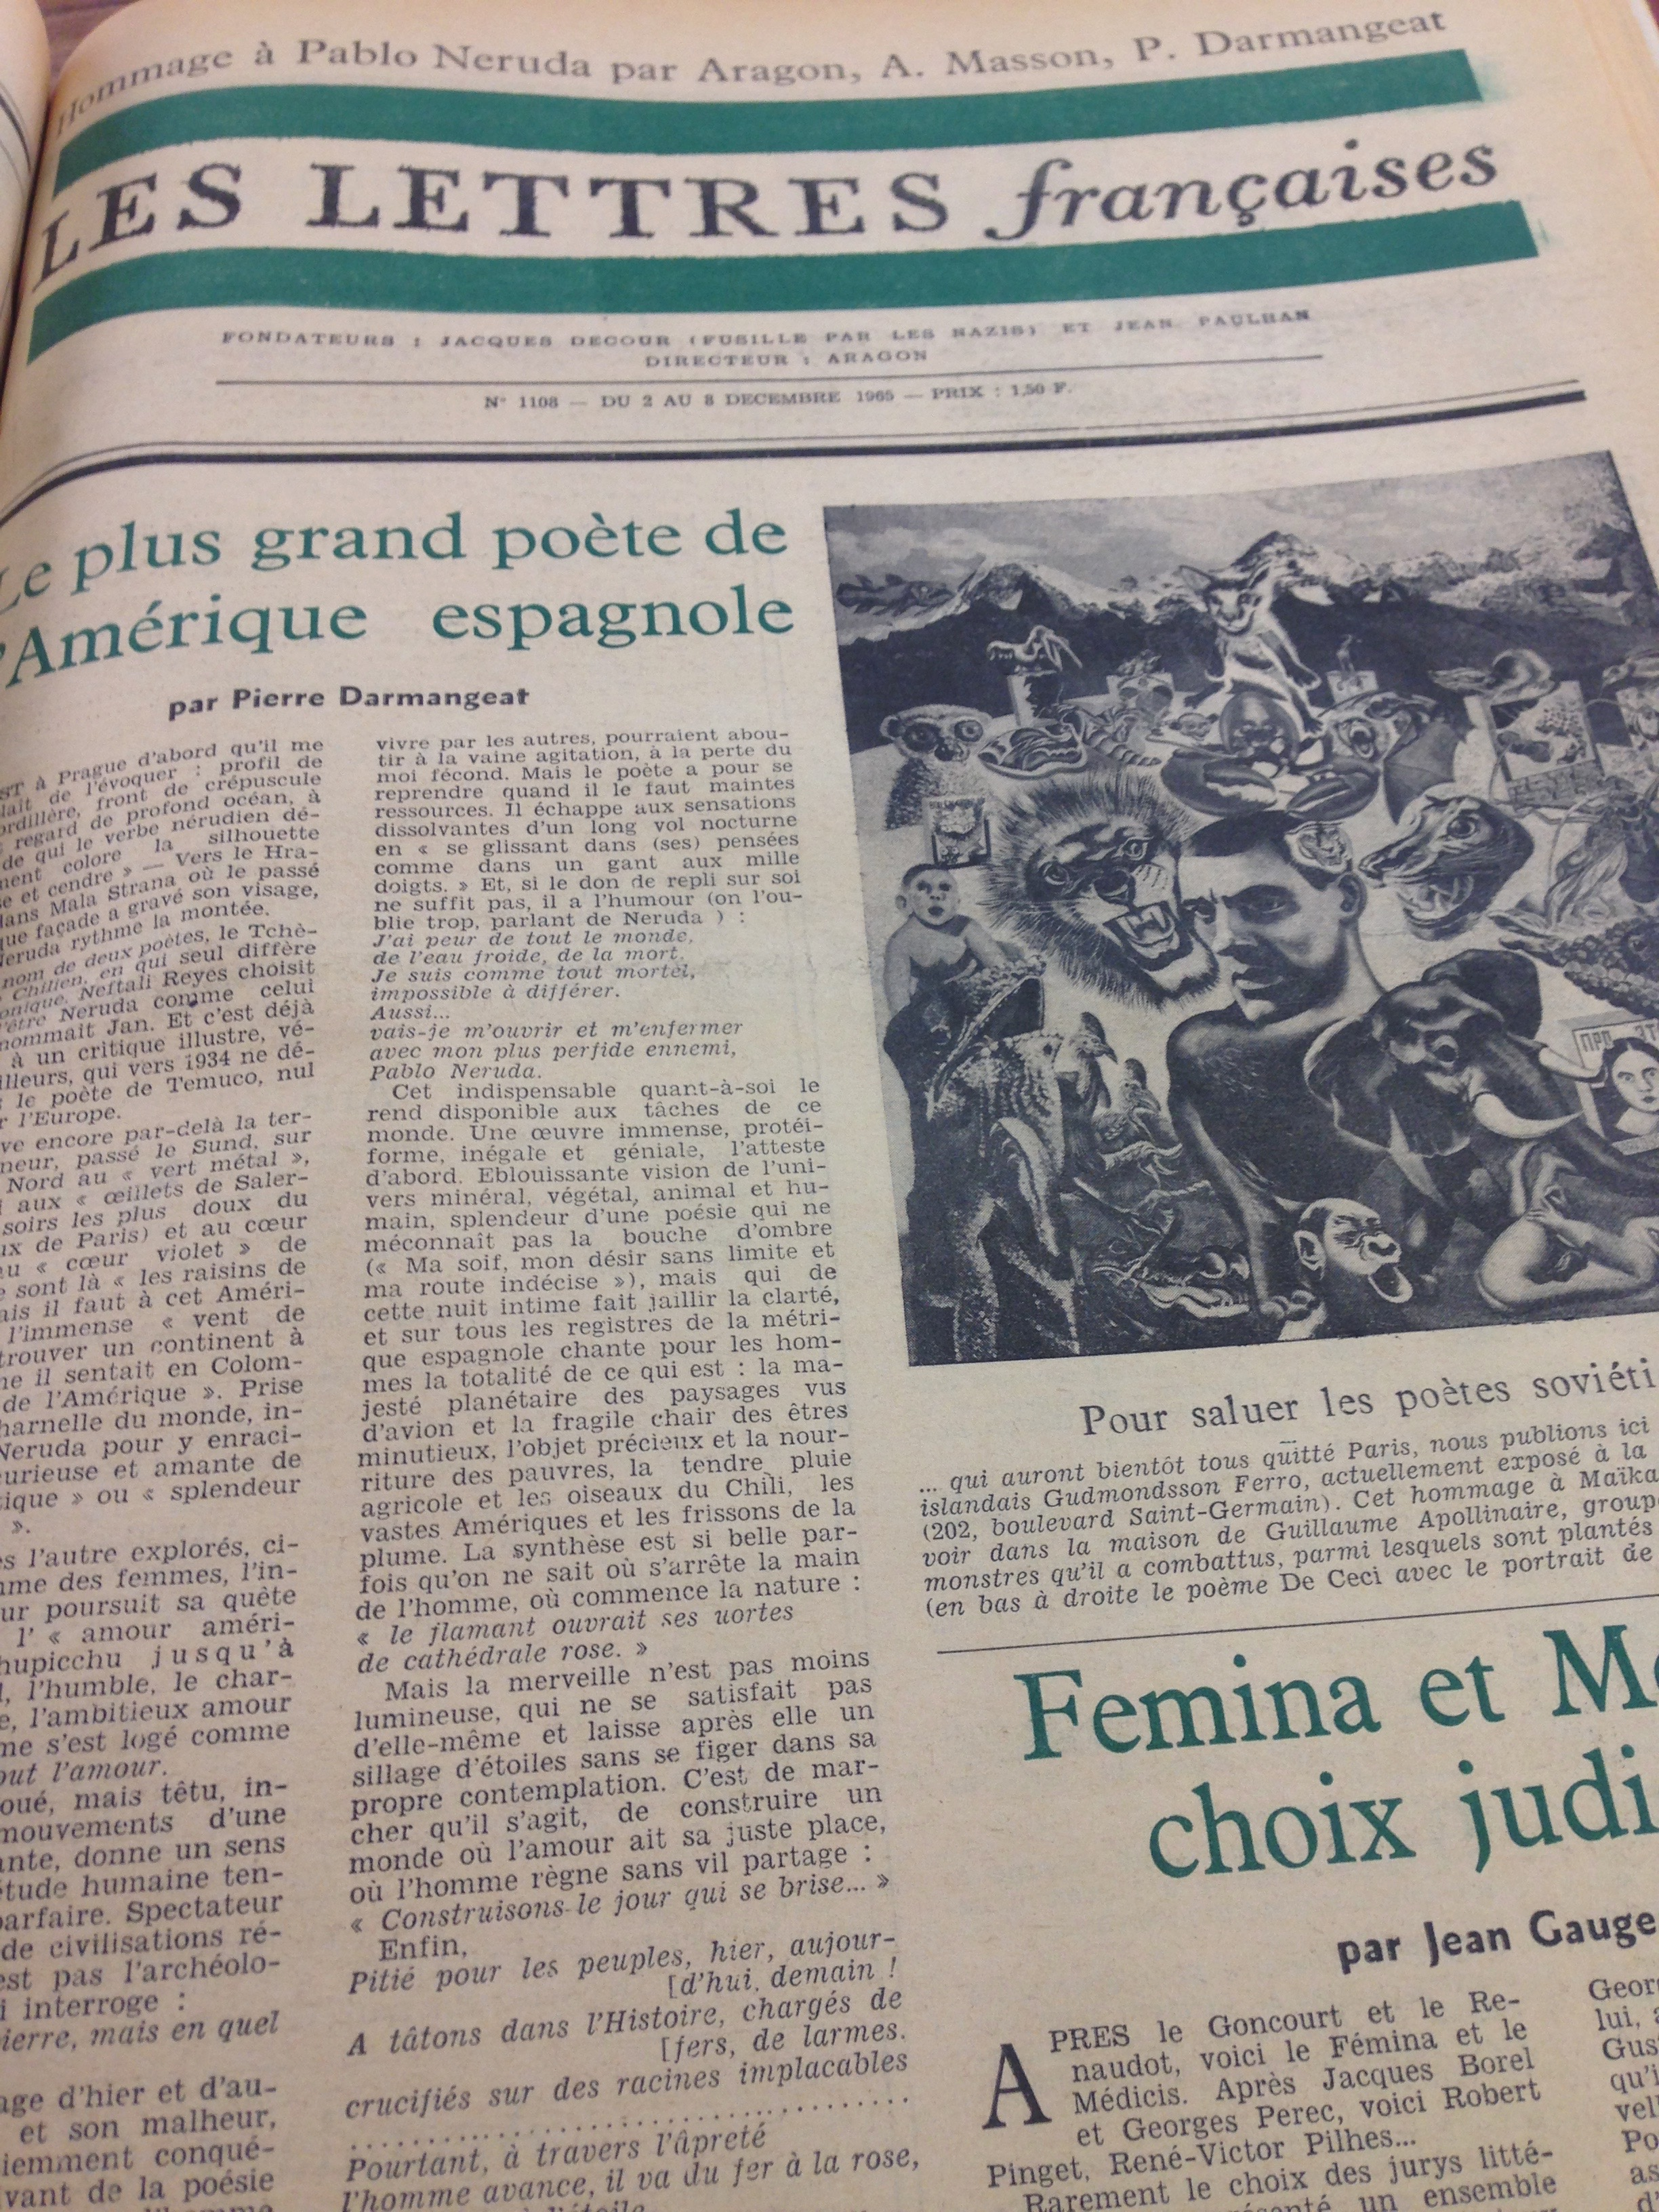
\includegraphics[width=\textwidth,height=\textheight,keepaspectratio]{Annexe/Image35.jpg}
	\caption{\cite{pabloneruda}}\label{fig:darmangeatneruda}
    \end{figure*}

    \begin{figure*}[htp]
   \centering
   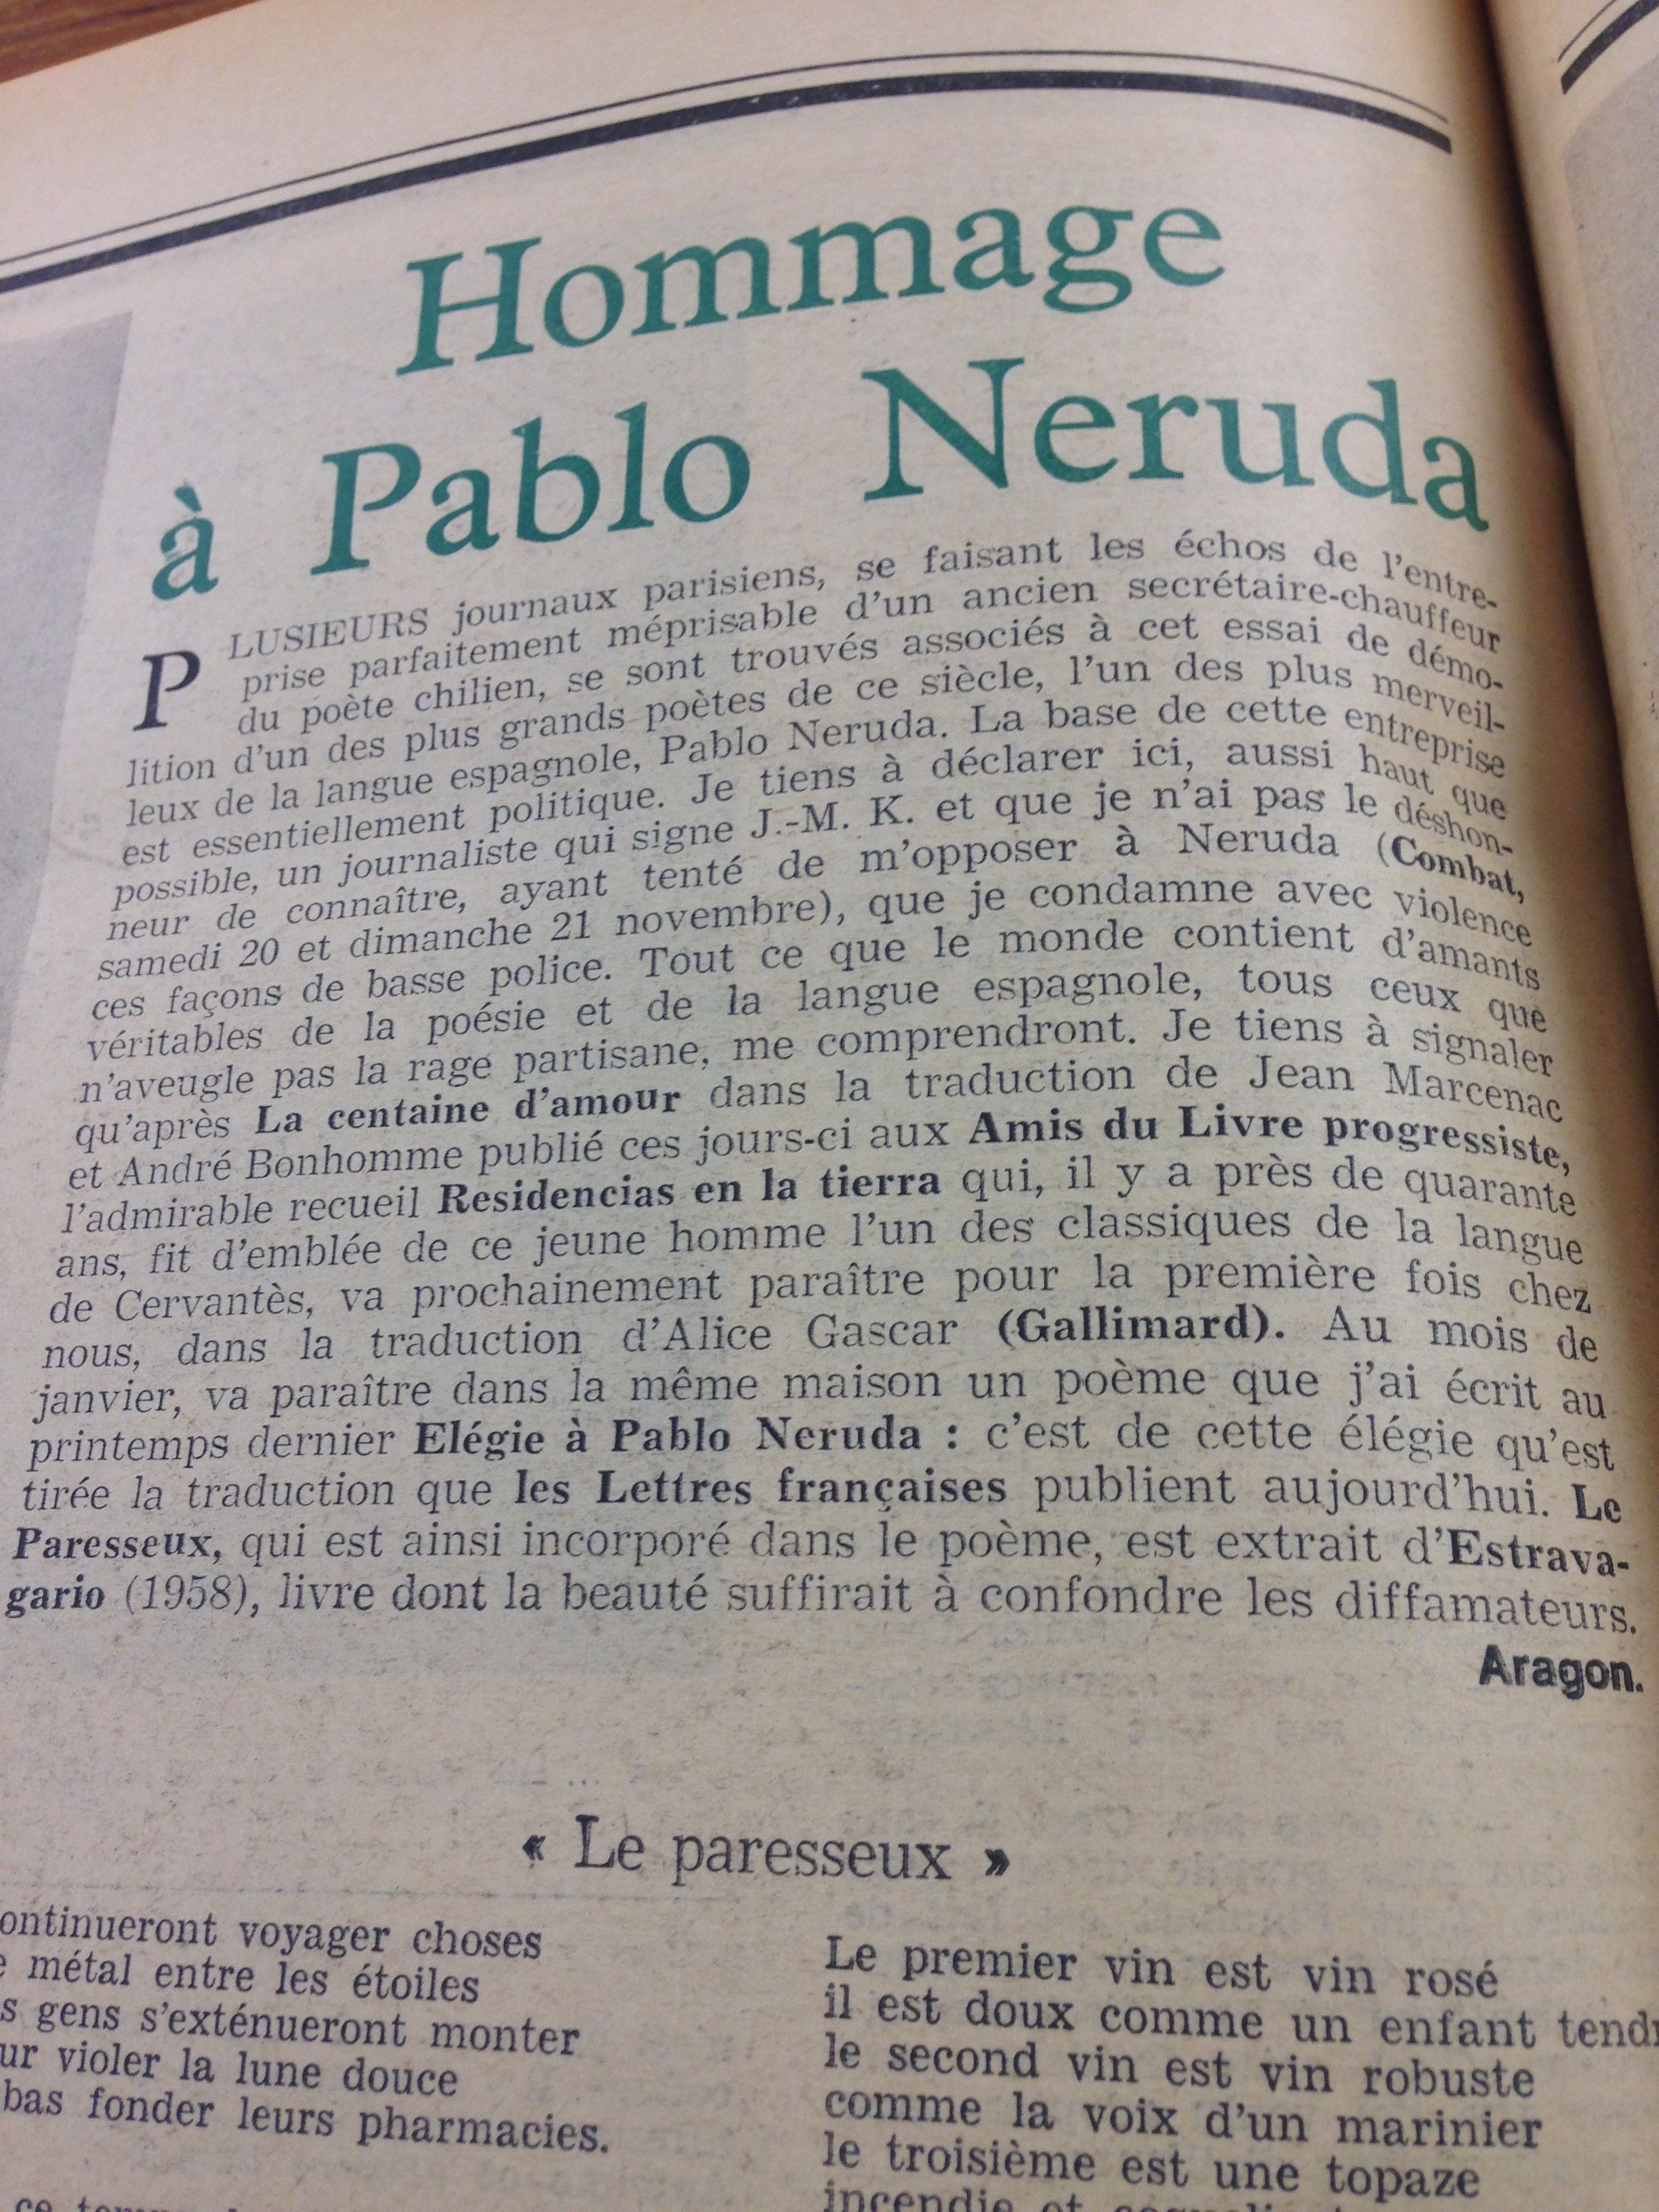
\includegraphics[width=\textwidth,height=\textheight,keepaspectratio]{Annexe/Image7.jpg}
	\caption{\cite{pabloneruda}}\label{fig:neruda2}
    \end{figure*}

    \begin{figure*}[htp]
   \centering
   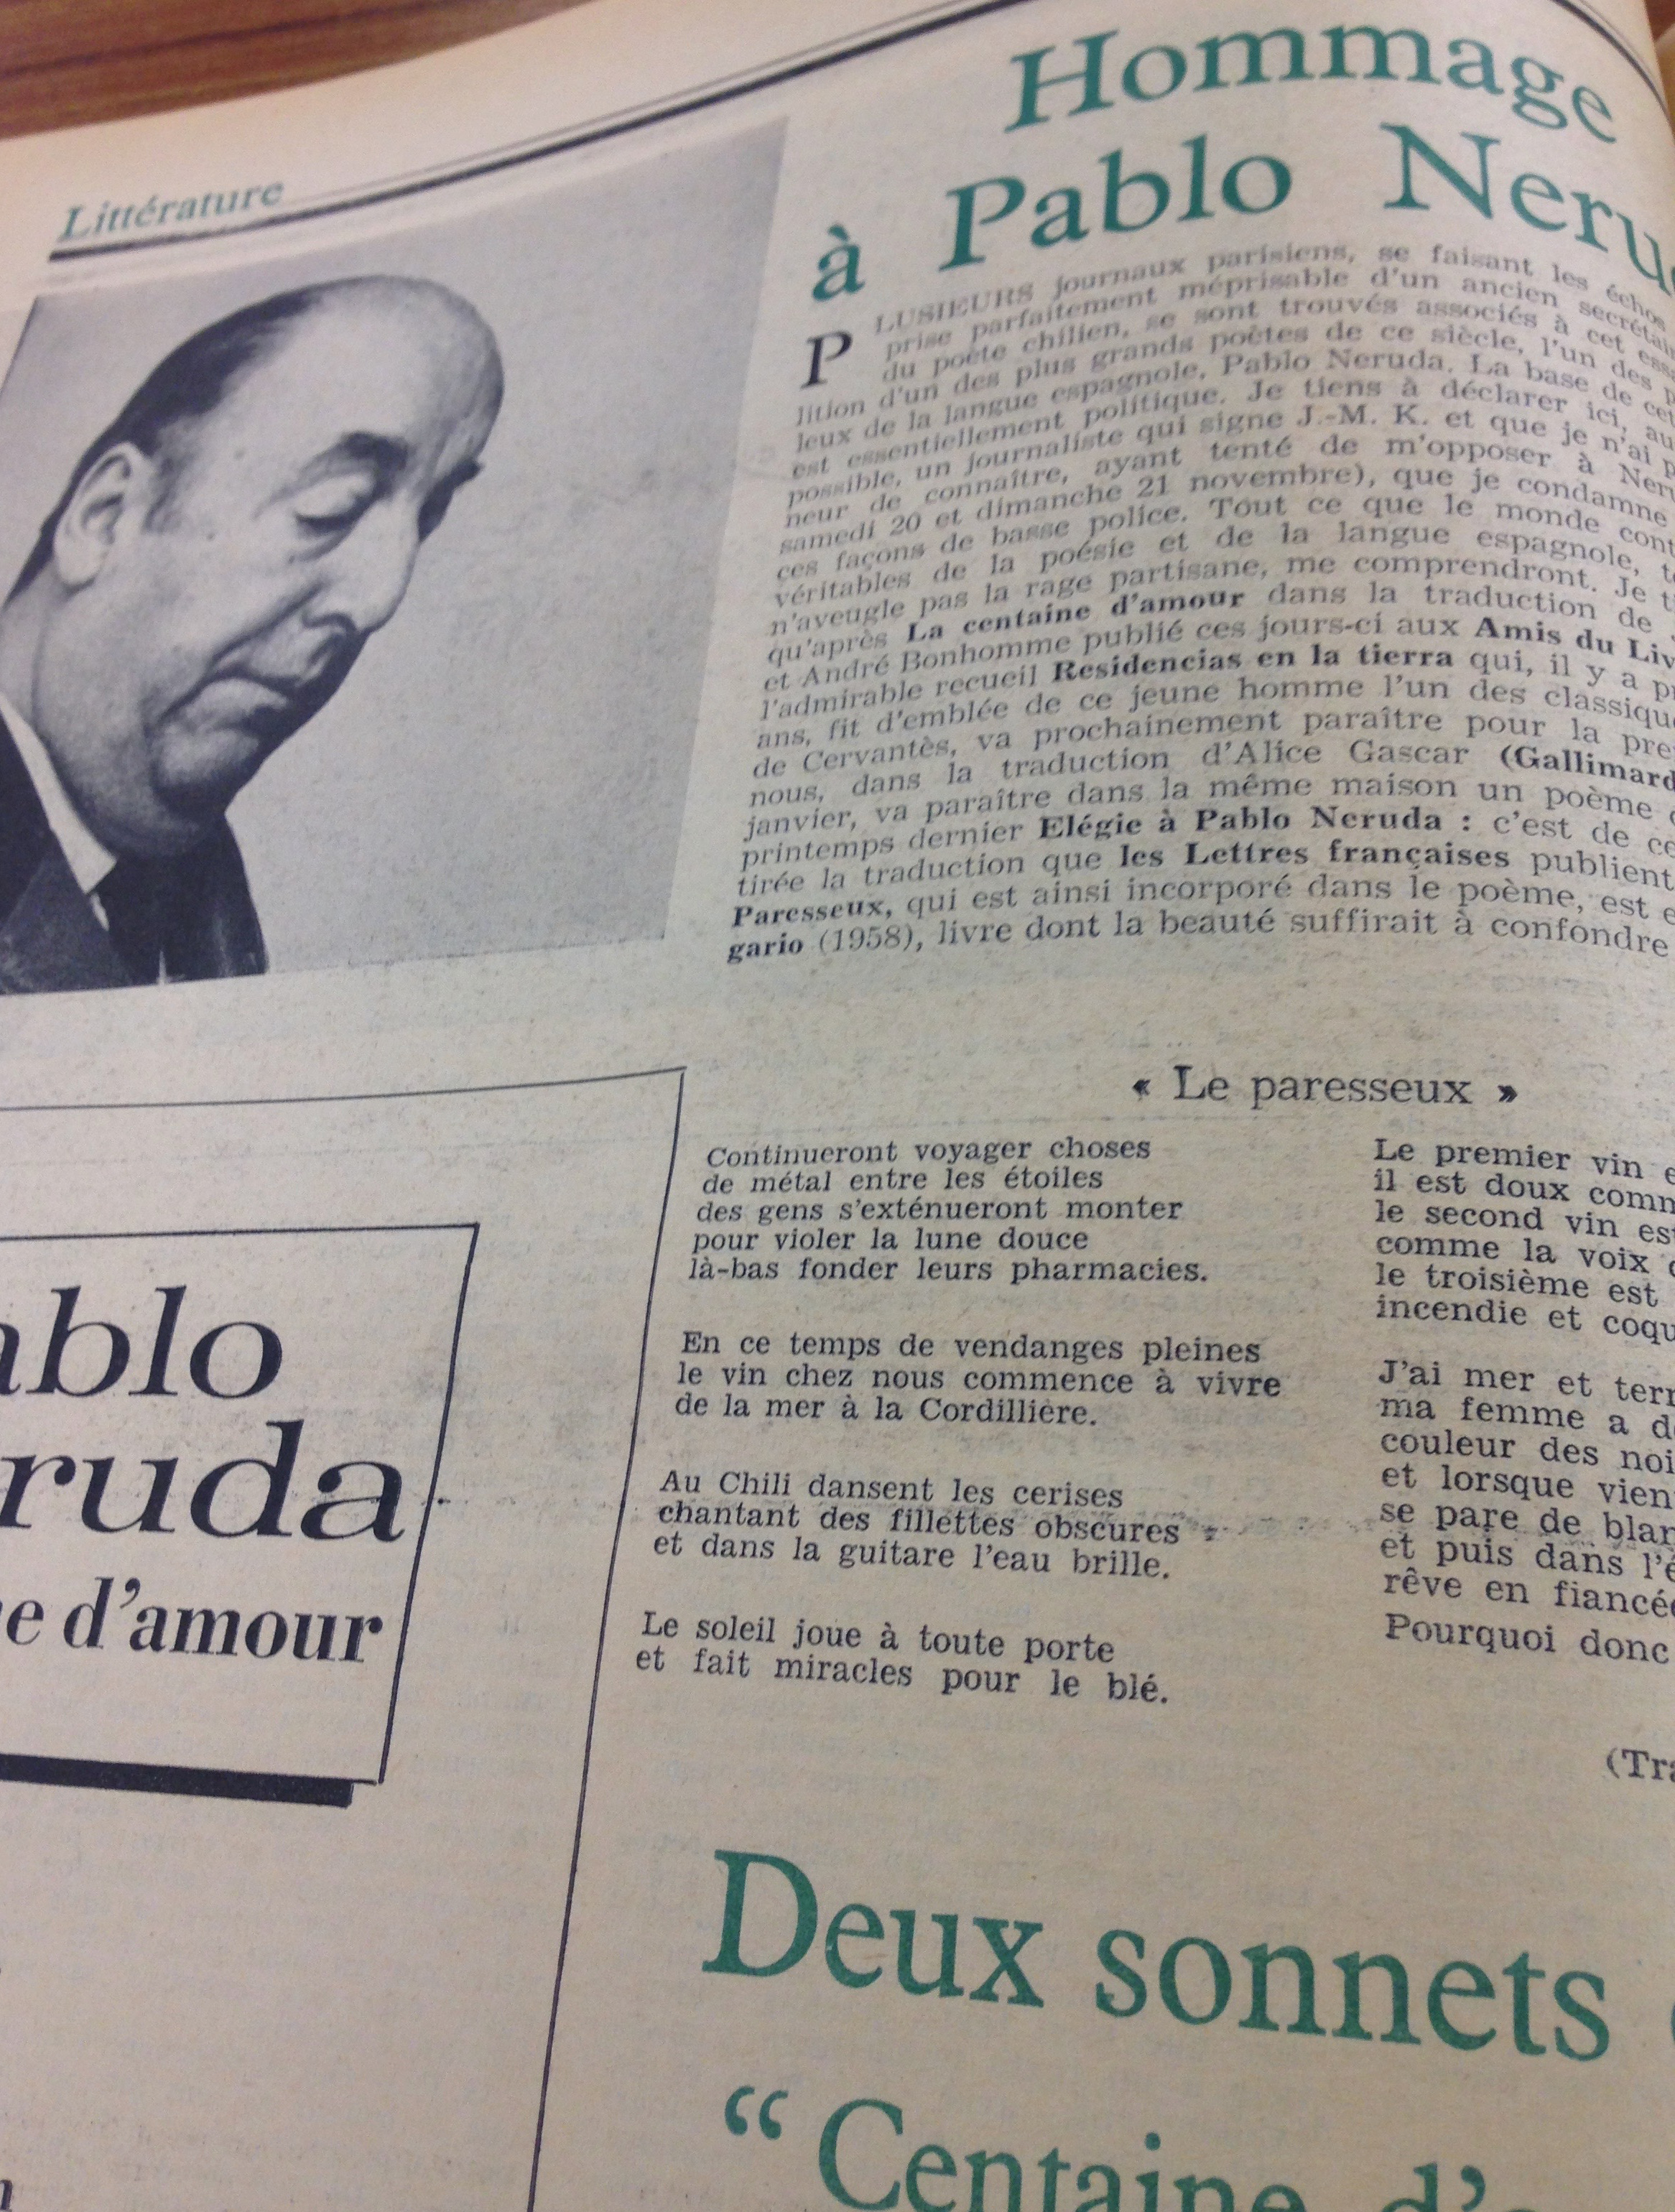
\includegraphics[width=\textwidth,height=\textheight,keepaspectratio]{Annexe/Image4.jpg}
	\caption{\cite{pabloneruda}}\label{fig:neruda}
    \end{figure*}


 
